% !TEX root = 22830110_dissertation.tex
\documentclass[12pt,a4paper]{report}

% Packages
\usepackage[utf8]{inputenc}
\usepackage[T1]{fontenc}
\usepackage{lmodern}
\usepackage[margin=1in]{geometry}
\usepackage{graphicx}
\usepackage{amsmath}
\usepackage{hyperref}
\usepackage{titlesec}
\usepackage{tocbibind}
\usepackage{setspace}
\usepackage{float}
\usepackage{enumitem}
\usepackage{caption}
\usepackage{subcaption}
\usepackage{booktabs}
\usepackage{tabularx}
\usepackage[round]{natbib}
\usepackage{microtype}
\usepackage{listings}
\usepackage{xcolor}

% Formatting
\onehalfspacing
\titleformat{\chapter}[display]{\normalfont\huge\bfseries}{\chaptertitlename\ \thechapter}{20pt}{\Huge}
\hypersetup{
    colorlinks=true,
    linkcolor=blue,
    filecolor=magenta,      
    urlcolor=cyan,
    citecolor=blue,
    pdftitle={Automating Year-End Accounting Notes},
    pdfauthor={Jatin Arora}
}
\lstset{
    basicstyle=\ttfamily\small,
    breaklines=true,
    frame=single,
    columns=fullflexible,
    keepspaces=true,
    showstringspaces=false,
    keywordstyle=\color{blue!60!black},
    commentstyle=\color{green!40!black},
    stringstyle=\color{red!50!black}
}

% Document Info
\title{
    \vspace{2cm}
    \textbf{Automating Year-End Accounting Notes}\\
    \Large An AI System to Generate Audit-Ready Financial Statement Notes from Xero Data
}
\author{
    \textbf{Jatin Arora}\\
    Student ID: 22830110\\
    Course: B.Sc. (Hons) Artificial Intelligence \& Data Science\\
    Supervisor: Dr. Mu. Mu.
}
\date{\today}

\begin{document}

% Title Page
\maketitle
\pagenumbering{roman}

% Abstract
% !TEX root = ../22830110_dissertation.tex
\begin{abstract}
\addcontentsline{toc}{chapter}{Abstract}
The generation of year-end accounting notes represents a critical but historically labour-intensive bottleneck in the financial reporting cycle. Under stringent regulatory frameworks such as IFRS and UK GAAP, accounting professionals must provide exhaustive narrative context to primary financial statements, a process that consumes substantial billable hours and introduces significant risks of human transcription errors. 

This dissertation presents the design, implementation, and evaluation of a novel multi-agentic AI framework for the automated synthesis of audit-ready accounting notes. The system bridges the gap between stochastic Large Language Model (LLM) generation and the deterministic requirements of financial auditing through two key architectural innovations: the \textit{Decimal Mandate} and a \textit{Sequential Multi-Agentic Orchestration} layer. The \textit{Decimal Mandate} enforces a zero-tolerance policy for floating-point approximations, using a deterministic data engineering pipeline that guarantees 100\% numeric fidelity prior to any generative synthesis. This is coupled with a CrewAI-based orchestration that decomposes the reporting task into specialised roles—Senior Financial Analyst, Accounting Partner, and Quality Control Reviewer—mimicking the hierarchical verification processes of a professional accounting firm.

Evaluation combined an 85-record accountant-authored validation corpus, a live benchmark subset of three representative long-form cases, and two human evaluation surveys with 10 professional respondents from Phipps Henson McAllister (PHM) UK. The live benchmark compared three GPT-5.4 prompt-engineering conditions with four callable GPT-4.1 fine-tuned deployments hosted in Azure AI Foundry. The results show a clear latency and behaviour trade-off: the strongest fine-tuned deployments produced drafts in roughly 12--15 seconds on average, the GPT-5.4 prompt baselines required roughly 64--72 seconds, and one fine-tuned deployment proved unstable by expanding to the output ceiling on a difficult case. The survey results reinforce the need for human review: manual drafting often exceeds one hour per note, and AI-generated drafts were rated as useful first drafts rather than autonomous final outputs.

The key contribution of this research is a verifiable, explainable-by-design pipeline that connects live cloud-accounting data (Xero API) with constrained generative AI, proving that AI, when governed by deterministic accounting rules, can augment professional judgement without compromising audit integrity. This research provides a scalable blueprint for the transition from manual compliance reporting to automated, high-fidelity financial storytelling.
\end{abstract}


% Acknowledgements
\chapter*{Acknowledgements}
\addcontentsline{toc}{chapter}{Acknowledgements}
I would like to express my deepest appreciation to my academic supervisors and the professionals at Phipps Henson McAllister (PHM) UK for their invaluable guidance and domain expertise throughout this project. Their insights into the intricacies of audit compliance and financial workflows were instrumental in shaping the requirements and evaluating the effectiveness of the ``ai\_review\_notes'' system.

\tableofcontents
\listoffigures
\listoftables

\clearpage
\pagenumbering{arabic}

% ---------------------------------------------------------
% !TEX root = ../22830110_dissertation.tex
\chapter{Introduction}
\label{chap:introduction}

\section{Background and Motivation}
Financial reporting forms the cornerstone of corporate accountability. Under frameworks such as the International Financial Reporting Standards (IFRS) and UK GAAP, year-end accounting notes are essential for providing the narrative context required to interpret balance sheets and income statements. However, the preparation of these notes remains a manual, highly labour-intensive process. Accounting professionals routinely consume significant billable hours navigating the meticulous demands of data verification, reconciliation, and compliance alignment. This inefficiency not only escalates costs—making detailed reporting financially unviable for smaller entities—but also heightens the risk of human error, potentially undermining audit integrity.

The emergence of Large Language Models (LLMs) offers a theoretical pathway to automation. Yet, the stochastic nature of these models introduces a critical paradox: accounting requires 100\% numeric fidelity, while LLMs are prone to "hallucinations" and mathematical approximations. Bridging this gap is not merely a task of prompt engineering, but a fundamental challenge of system architecture.

\section{The Research Gap: From Stochastic Text to Deterministic Audit}
While recent advancements in Artificial Intelligence have revolutionized fields from medical imaging to creative writing, its adoption in high-stakes financial auditing has been hampered by a significant research gap. Current AI systems in finance often focus on isolated components—such as anomaly detection or simple data extraction—but fail to integrate deterministic data engineering with constrained generative synthesis. 

Existing Literature often treats LLMs as black-box calculators. There is a documented lack of frameworks that:
\begin{enumerate}
    \item Enforce absolute numeric precision (avoiding floating-point errors) in AI-generated narratives.
    \item Implement multi-layered human-in-the-loop verification that mimics the hierarchical structure of professional firms.
    \item Provide granular, transaction-level provenance for every generated statement.
\end{enumerate}
This dissertation addresses this gap by introducing a hybrid architecture that treats the LLM not as a calculator, but as a \textit{narrative synthesizer} governed by a deterministic rules engine.

\section{Research Question and Objectives}
The central research question of this study is: \textit{To what extent can a multi-agentic AI framework, constrained by deterministic data engineering, automate the production of IFRS/GAAP-compliant accounting notes without compromising numeric accuracy or auditability?}

To address this, the project pursues the following objectives:
\begin{enumerate}
    \item To design and implement a \textbf{Decimal Mandate} architecture for 100\% precise data extraction from the Xero API.
    \item To develop a \textbf{Multi-Agentic Orchestration} layer using CrewAI to simulate professional verification workflows.
    \item To conduct a \textbf{Benchmarking Study} across 10 distinct LLMs to identify the optimal architecture for financial narrative synthesis.
    \item To evaluate the system through a \textbf{Human-in-the-Loop study} with professional accountants, measuring time savings and professional acceptability.
\end{enumerate}

\section{Contribution and Significance}
The primary contribution of this research is the \textbf{ai\_review\_notes} framework, an end-to-end pipeline that demonstrates the viability of "Explainable AI by Design" in professional accounting. Key innovations include:
\begin{itemize}
    \item \textbf{The Decimal Mandate:} A novel data engineering methodology that isolates LLMs from mathematical reasoning, ensuring numeric outputs are sourced only from deterministic code.
    \item \textbf{Agentic Separation of Concerns:} A framework where specialised AI agents (Analyst, Writer, Reviewer) provide the checks and balances necessary for audit-grade outputs.
    \item \textbf{Practical Workflow Evidence:} Survey and benchmark evidence showing that year-end note drafting is time-consuming in practice and that AI-generated drafts are useful when kept inside a professional review loop.
\end{itemize}

\section{Dissertation Structure}
The remainder of this dissertation is structured as follows: Chapter \ref{chap:literature_review} provides a critical review of the state-of-the-art in financial AI and XAI. Chapter \ref{chap:aim_and_objectives} further defines the technical aims. Chapter \ref{chap:analysis_design} details the system's architectural layers. Chapter \ref{chap:methodology} deep-dives into Transformer theory and the comparative test harness for the GPT-5.4 prompting baseline and the live GPT-4.1 fine-tuned deployments. Chapter \ref{chap:implementation} discusses the technical realisation, followed by Chapter \ref{chap:testing_evaluation} which presents the experimental results. Finally, Chapter \ref{chap:conclusions} summarises the findings and outlines future research pathways.
 

% !TEX root = ../22830110_dissertation.tex
\chapter{Literature Review}
\label{chap:literature_review}

\section{Introduction to the Literature}
Financial reporting forms the cornerstone of corporate accountability, ensuring stakeholders can assess organisational health through transparent disclosures mandated by standards such as International Financial Reporting Standards (IFRS) and Generally Accepted Accounting Principles (GAAP). Year-end accounting notes, particularly those detailing fixed assets, accruals, and related-party transactions, are essential for compliance. However, preparing these notes manually is labour-intensive, consuming numerous billable hours due to meticulous data verification, reconciliation across sources, and alignment with evolving regulatory requirements. 

The advent of artificial intelligence (AI) promises to transform this landscape by automating data extraction, numeric reconciliation, and text generation. Advances in natural language processing (NLP), including large language models (LLMs) and retrieval-augmented generation (RAG), enable the conversion of structured bookkeeping data into compliant narrative disclosures. Yet, AI outputs must adhere to strict accounting rules to avoid hallucinations, while ethical concerns demand robust frameworks. Existing studies often focus on isolated components like anomaly detection or fraud prevention, but rarely integrate deterministic data engineering with constrained generative techniques.

This chapter synthesizes evidence on automating year-end accounting notes through AI systems that generate compliant financial statement disclosures from sources like Xero. It examines accounting standards, financial data engineering, NLP innovations for data-to-text generation, and ethical considerations in explainable AI (XAI).

\section{Methodology of the Review}
\subsection{Search Strategy and Study Selection}
A comprehensive search was performed across academic databases employing hybrid semantic and keyword-based retrieval to maximise coverage. Search queries targeted IFRS/GAAP compliance, Xero API and ETL data engineering, NLP and LLM data-to-text generation, and AI ethics in accounting.

Initial searching identified 360 records. After duplicate removal and relevance-based filtering, 100 records were screened against eligibility criteria, resulting in 20 papers included in the final synthesis. Eligibility criteria demanded a focus on accounting practices, AI technology integration, publication post-2010, evidence quality, and practical application.

\subsection{Data Extraction and Synthesis}
Data extraction focused on accounting standards, data engineering methods (including ETL and numeric reconciliation), NLP and AI techniques (LLMs, RAG, hallucination mitigation), and ethical considerations (XAI, provenance tracking). Thematic analysis identified patterns and synthesized findings across studies. The included studies, spanning 2020 to 2025, predominantly feature technical analyses, case studies, and empirical evaluations in financial auditing and accounting contexts \cite{Tripathi2025b, Nath2025b, Zhong2024}.

\section{Thematic Findings}

\subsection{Accounting Standards and Disclosure Practices}
Mandatory year-end notes under IFRS and GAAP demand extensive verification to ensure transparency, rendering manual preparation highly time-consuming and prone to errors \cite{Rushi2025a, Rushi2025b}. These disclosures require reconciling transaction data with standards to map errors to specific violations. Studies consistently highlight inefficiencies in traditional processes, such as periodic manual sampling, which fail to scale with complex datasets from multiple sources. Manual approaches contrast sharply with automated potentials, where inefficiencies in handling fixed asset valuations and accrual recognitions lead to overlooked irregularities.

\subsection{Financial Data Engineering for Extraction, Reconciliation, and Traceability}
Robust data reconciliation strategies, including anomaly detection and integration from fragmented sources, enhance numeric accuracy for compliance reports. Cloud-native frameworks enable scalable ETL processes via Python orchestration and SQL validation rules to process transactions at scale \cite{Tripathi2025b, Badugu2025}. These methods ensure traceability through automated exception management and real-time monitoring, outperforming manual reconciliation by reducing error risks in large datasets. Automation tools like Audit Command Language (ACL) and robotic process automation (RPA) facilitate data import, cleaning, and numeric reconciliation \cite{Rout2020a, Rout2020b}. 

\subsection{NLP and Data-to-Text Advances in Accounting with LLM and RAG Integration}
LLMs automate financial statement auditing by identifying errors in curated datasets, using multi-stage frameworks to assess capabilities, though they sometimes struggle with explaining detections and citing IFRS/GAAP standards \cite{Rushi2025a, Rushi2025b}. RAG agents revolutionize bookkeeping by leveraging vector databases for semantic transaction understanding, achieving superior accuracy in categorization and cross-verification over rule-based systems \cite{Vemulapalli2025}. Human feedback loops mitigate hallucinations through grounded retrieval. These techniques augment professionals by reducing verification time, enabling data-to-text generation for compliant disclosures \cite{Brij2025}.

\subsection{Ethics, Trust, and Explainable AI in Audit Automation}
XAI enhances trust in auditing by integrating explainability layers for fraud detection, providing interpretable decisions that align with regulations while human-in-the-loop feedback ensures oversight \cite{Zhong2024, Vardhan2021}. Ethical risks, including bias and opacity in AI models, are mitigated through techniques like SHAP and LIME, which build auditor confidence, alongside provenance tracking via traceable datasets \cite{Boggavarapu2025, Bran2024}. Continuous auditing with models like XGBoost and Transformers balances accuracy and interpretability, emphasizing hybrid systems for transparency \cite{Wibowo2025}.

\section{Discussion}

\subsection{Principal Findings and Their Interpretation}
The synthesis demonstrates that AI integration in financial auditing yields robust efficiency gains, particularly through data reconciliation frameworks that scale numeric verification, enabling seamless transitions to generative text outputs for year-end notes. Automated ETL pipelines create verifiable foundations that LLMs can build upon without fabricating details. The success of RAG in grounding semantic analysis reflects its mechanistic advantage: it enforces factual alignment with transaction records, directly countering LLM hallucinations. XAI's interpretability fosters trust by revealing how inputs influence outputs.

These findings suggest hybrid viability for audit-ready notes: numeric reconciliation acts as a deterministic gatekeeper, ensuring data integrity before constrained LLM generation. The evidence confidently supports AI as an enhancer of professional judgement, aligning with augmentation paradigms.

\subsection{Comparison with Existing Literature}
The reviewed findings align with prior work emphasizing productivity augmentation, where tools like RAG extend human cognition by providing contextual retrieval. Efficiency gains in transaction categorization consistently outperform rule-based systems, which falter on ambiguity. XAI's reduction of false positives allows auditors to validate outputs against standards, reinforcing trust \cite{Zhong2024}. While earlier studies warned of opacity risks, methodological evolution from RPA-focused automation to Transformer models suggests a progression toward hybrid reliability.

\subsection{Practical Implications}
Accounting firms stand to benefit most from hybrid AI systems, where numeric reconciliation frameworks preprocess data for RAG-enhanced note generation, cutting billable hours on disclosures by automating verification. Implementing XAI ensures compliance without opacity risks. Practitioners should integrate human oversight in loops for high-stakes related-party notes, validating LLM outputs against standards to mitigate hallucinations. Regulatory bodies could mandate XAI provenance tracking for audits, requiring no-threshold transparency \cite{Maknickiene2025}.

\section{Gaps and Future Directions}
The synthesis uncovers gaps in integrating numeric reconciliation with constrained LLM generation. Studies emphasize isolated components—reconciliation in cloud frameworks \cite{Badugu2025} or RAG for text \cite{Vemulapalli2025}—but lack end-to-end systems from Xero data to produce IFRS/GAAP-compliant notes. Mechanistic evidence on hallucination propagation in accounting pipelines is absent. Future studies should conduct real-world trials directly testing hybrid prototypes on Xero-extracted datasets for year-end notes, implementing harmonized benchmarks with exact compliance metrics.

\section{Conclusion}
Automating year-end accounting notes via an AI system that generates audit-ready disclosures from Xero data is feasibly advanced by combining deterministic numeric reconciliation with constrained LLM and RAG techniques. LLMs successfully identify discrepancies, RAG enhances semantic accuracy, and XAI models deliver interpretable results, collectively reducing manual burdens without supplanting professional roles. This review underscores the transformative potential of these systems for regulatory transparency and cost savings in financial reporting.

% !TEX root = ../22830110_dissertation.tex
\chapter{Aim and Objectives}
\label{chap:aim_and_objectives}

\section{Aim}
The primary aim of this project is to design, implement, and evaluate a prototype system—\textit{ai\_review\_notes}—that automatically generates year-end accounting notes from Xero data, providing auditable numeric reconciliations, explanatory narrative, and strict provenance sufficient for an accountant to efficiently review and sign-off.

\section{Objectives}
To achieve this aim, the project is broken down into seven concrete objectives:
\begin{enumerate}
    \item \textbf{Target Selection:} Select and define 3–5 target note types to automate, including critical areas such as Fixed Assets, Directors' Remuneration, and Debtors/Creditors.
    \item \textbf{Data Pipeline Setup:} Build a reproducible ETL pipeline to extract, transform, and securely store relevant bookkeeping data directly from the Xero API.
    \item \textbf{Deterministic Rules Engine:} Define accounting mapping tables and deterministic rules to compute the numeric backbone for each note, strictly adhering to the ``Decimal Mandate'' (avoiding floating-point errors).
    \item \textbf{Provenance Modelling:} Develop a provenance model linking every computed figure and variance (>10\% materiality threshold) to its source transactions or journal entries.
    \item \textbf{LLM Synthesis Generation:} Implement a note generation module using a multi-agentic LLM framework (CrewAI) with heavily constrained prompts and templates to enforce firm-standard narrative styling.
    \item \textbf{Human-in-the-Loop Evaluation:} Design and execute a human evaluation study involving professional accountants to systematically measure factual accuracy, professional acceptability, edit distances, and time savings.
    \item \textbf{Analysis and Compliance Review:} Analyse the results, meticulously document system limitations, and propose improvements regarding explainability, ethical boundaries, and UK GAAP compliance.
\end{enumerate}

\section{Research Questions}
To guide the investigation and achieve the aforementioned aim and objectives, this dissertation addresses the following core research questions:
\begin{enumerate}[label=\textbf{RQ\arabic*:}]
    \item \textbf{Efficiency and Fidelity:} To what extent can an AI-driven, multi-agentic system automate the drafting of year-end accounting notes, and can it maintain 100\% numeric accuracy through strict deterministic constraints (the ``Decimal Mandate'')?
    \item \textbf{Hallucination Mitigation:} How effectively does the integration of a verifiable provenance model and pre-synthesis data reconciliation mitigate the risk of Large Language Model (LLM) hallucinations in high-stakes financial reporting?
    \item \textbf{Model Comparative Performance:} Among current state-of-the-art LLMs (e.g., GPT-4o, Claude 3.5 Sonnet, Llama 3), which architectures yield the most reliable, accurate, and stylistically appropriate outputs for UK GAAP/IFRS compliance?
    \item \textbf{Professional Acceptability:} How do human-in-the-loop professional accountants evaluate the readability, professional tone, and overall utility of the AI-generated drafts as viable starting points for audit sign-offs?
\end{enumerate}

% !TEX root = ../22830110_dissertation.tex
\chapter{Analysis and Design of the Proposed Solution}
\label{chap:analysis_design}

\section{System Requirements and Constraints}
Developing software for financial compliance introduces exceptionally rigorous constraints. A single rounding error or unverified assumption can invalidate an entire financial report. The analysis phase identified three primary layers required for the architecture:
\begin{enumerate}
    \item \textbf{Ingestion (ETL) Layer:} Securely handling Xero OAuth2 authentication, extracting transactional data, and normalising it into a deterministic format.
    \item \textbf{Rules Engine (Core Layer):} A deterministic mathematical engine. This layer computes variances and Prior-Year (PY) comparisons. It enforces the ``Decimal Mandate,'' strictly prohibiting \texttt{float} data types in favor of \texttt{decimal.Decimal} with \texttt{ROUND\_HALF\_UP}. It also integrates robust statistical analysis on historical transactions to identify material drivers, recurring subscriptions, and potential anomalies prior to the synthesis phase.
    \item \textbf{Synthesis (NLG Layer):} The Natural Language Generation layer, responsible for translating the deterministic numeric outputs into human-readable, professional narrative.
\end{enumerate}

\section{Firm-Standard Variance Logic and Triggers}
The system design incorporates specific materiality thresholds. The AI must flag and generate commentary for variances greater than 10\%. Trivial changes are filtered out, except for ``Mandatory Comment Accounts'' which require commentary regardless of variance magnitude. These include Directors' Remuneration, Legal \& Professional Fees, Donations \& Entertainment, and Bad Debts.

\section{Security, Privacy, and Anonymisation}
Because the system handles sensitive financial data, compliance with UK GDPR is a basic requirement. The design follows the core principles highlighted in the UK Information Commissioner's Office (ICO) guidance: purpose limitation, data minimisation, storage limitation, integrity/confidentiality, and accountability (\url{https://ico.org.uk/for-organisations/uk-gdpr-guidance-and-resources/data-protection-principles/a-guide-to-the-data-protection-principles/}). The system is framed as a draft-generation tool for year-end working papers only; it is not a general-purpose document store or autonomous filing agent.

An Anonymisation Layer (DataMasker) was designed to redact Personally Identifiable Information (PII) such as director names, sensitive supplier names, personal addresses, and free-text references that could expose natural persons. This reflects the ICO's data-minimisation expectation that organisations should process only data that is adequate, relevant, and limited to what is necessary for the stated purpose (\url{https://ico.org.uk/for-organisations/uk-gdpr-guidance-and-resources/data-protection-principles/a-guide-to-the-data-protection-principles/data-minimisation/}). Where redaction would materially damage accounting meaning, the design instead prefers pseudonymisation and controlled access for authorised reviewers.

The system also raises specific privacy concerns in a professional-services context:
\begin{itemize}
    \item \textbf{Director and employee data:} payroll narratives, directors' loan accounts, and benefits-in-kind commentary may expose personal financial behaviour.
    \item \textbf{Supplier and customer identification:} one-off payees, legal advisers, and related-party entities may reveal commercially sensitive relationships.
    \item \textbf{Retention risk:} prompts, completions, and exported logs must not be kept indefinitely once the review cycle is complete, in line with the storage-limitation principle (\url{https://ico.org.uk/for-organisations/uk-gdpr-guidance-and-resources/data-protection-principles/a-guide-to-the-data-protection-principles/storage-limitation/}).
    \item \textbf{Human oversight:} because generated notes may contain hallucinated or misattributed commentary, a qualified accountant remains accountable for final review before any client-facing use.
\end{itemize}

\begin{figure}[H]
    \centering
    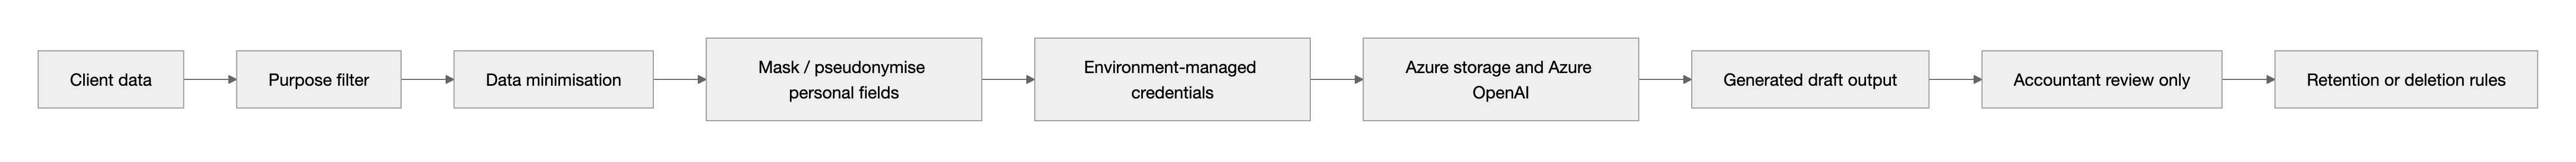
\includegraphics[width=0.72\textwidth]{figures/privacy_controls_flow}
    \caption{Privacy and Control Gates Applied to Client Data Before and After Generation}
    \label{fig:privacy_controls_flow}
\end{figure}

Figure \ref{fig:privacy_controls_flow} summarises the control path assumed in the design. The main point is that the model should not be treated as the first place where privacy is considered. Purpose filtering, minimisation, masking, credential handling, accountant-only review, and retention controls all sit around the generation step.

The cloud deployment choice was also influenced by provider privacy controls. Microsoft states that prompts, completions, and fine-tuning data sent to Azure OpenAI are not shared with other customers, are not available to OpenAI, and are not used to train or improve the foundation models (\url{https://learn.microsoft.com/en-us/legal/cognitive-services/openai/data-privacy}). This does not remove the need for local controls, but it does make the Azure-hosted deployment materially more appropriate than consumer-grade tooling for professional accounting data. In other words, Azure was chosen not merely for convenience, but because the project required a platform with enterprise data-protection guarantees that were more compatible with handling confidential company working-paper material.

This security posture also affects what can be submitted publicly. The dissertation repository includes the code required to reproduce the pipeline and evaluation workflow, but it does not include live \texttt{.env} credential files or active service secrets. Those values provide access to protected company-connected resources and therefore fall outside the scope of safe academic submission. A supervised live demonstration of the system is instead available on request.

\section{Interface and User Experience Design}
The design of the application's interface was governed by the requirement for "Clarity over Decoration." Financial professionals require a tool that minimizes cognitive load while maximizing data visibility. 

The user interface was designed with a "Side-by-Side Review" paradigm. This allows the user to see the raw financial data on the left and the AI-generated narrative on the right, facilitating immediate verification. The interface also incorporates "Confidence Scoring" and "Provenance Tracking," where specific numeric values in the narrative are linked back to their source ledger entries, creating a transparent and audit-ready review environment.

\subsection{Wireframe Architecture and User Journey}
The design phase involved the creation of low-fidelity and high-fidelity wireframes to map the accountant's workflow. This journey was segmented into three primary stages:
\begin{enumerate}
    \item \textbf{Secure Ingress:} A streamlined authentication interface designed to emphasize data security from the first interaction.
    \item \textbf{Client Monitoring Workbench:} A data-dense dashboard providing a high-level overview of the entire client portfolio, enabling accountants to manage multiple review cycles simultaneously without navigational friction.
    \item \textbf{The Synthesis Hub:} The primary interaction point where the "Side-by-Side Review" logic is implemented. This hub allows users to provide direct feedback to the AI for narrative regeneration, bridging the gap between automated drafting and human professional judgement.
\end{enumerate}

% !TEX root = ../22830110_dissertation.tex
\chapter{Methodology}
\label{chap:methodology}

\section{Introduction}
This chapter outlines the methodological framework used to design, build, and evaluate the AI-driven financial note generation system. It begins with the underlying architecture of modern Large Language Models (LLMs), in particular the Transformer. It then sets out the deployment infrastructure, the multi-agent architecture implemented with CrewAI, and the benchmarking framework used to compare the GPT-5.4 prompting baseline with the callable GPT-4.1 fine-tuned deployments produced from the project training recipes.

\section{Deep Dive: The Architecture of Transformers}
Prior to 2017, the dominant architectures for Natural Language Processing (NLP) were Recurrent Neural Networks (RNNs) and their more advanced variant, Long Short-Term Memory (LSTM) networks. While effective for short sequences, these models processed data sequentially, which inherently limited their ability to scale across parallel hardware and often caused them to "forget" earlier context in long documents. 

The publication of "Attention Is All You Need" by Vaswani et al. (2017) introduced the Transformer, an architecture that dispensed entirely with recurrence and convolutions in favor of an "attention" mechanism. This paradigm shift forms the foundational technology for all modern LLMs, including the ones used in this research.

\subsection{Self-Attention Mechanism}
At the core of the Transformer is the self-attention mechanism, which allows the model to determine the relevance of all other words in a sequence when encoding a specific word. In the context of financial accounting, this means the model can dynamically link a referenced "accrual" on page five to the specific "invoice date" mentioned on page one.

The mechanism operates by mapping a query and a set of key-value pairs to an output. For each word (token) in the input, three vectors are created through learned linear transformations: a Query vector (\$Q\$), a Key vector (\$K\$), and a Value vector (\$V\$). 

The attention score is computed using the scaled dot-product attention formula:
\begin{equation}
\text{Attention}(Q, K, V) = \text{softmax}\left(\frac{QK^T}{\sqrt{d_k}}\right)V
\end{equation}
where $d_k$ is the dimension of the key vectors. The dot product of the query with all keys dictates the weight (or focus) placed on each corresponding value. The division by $\sqrt{d_k}$ serves to scale the gradients, preventing them from vanishing or exploding during training.

\subsection{Multi-Head Attention and Positional Encoding}
Rather than performing a single attention function, Transformers use "Multi-Head Attention." This allows the model to jointly attend to information from different representation subspaces at different positions. For instance, one "head" might learn to attend to grammatical structure, while another attends to numeric relationships—a critical feature when parsing a Trial Balance.

Because the Transformer processes all tokens simultaneously, it lacks inherent knowledge of word order. To rectify this, positional encodings are added to the input embeddings at the bottoms of the encoder and decoder stacks. These encodings inject information about the relative or absolute position of the tokens in the sequence, using sine and cosine functions of different frequencies.

\subsection{Encoder vs. Decoder Architectures}
The original Transformer featured both an encoder (to map the input to a continuous representation) and a decoder (to generate the output sequence). Subsequent architectures diverged based on their use cases:
\begin{itemize}
    \item \textbf{Encoder-Only (e.g., BERT):} Excellent for tasks requiring deep bidirectional understanding, such as sentiment analysis or named entity recognition.
    \item \textbf{Decoder-Only (e.g., GPT series):} Optimised for autoregressive text generation. These models predict the next token based on all previous tokens, making them ideal for generating the narrative of a year-end accounting note.
\end{itemize}

\begin{figure}[H]
    \centering
    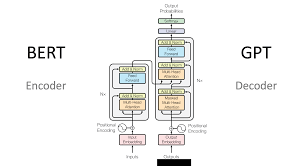
\includegraphics[width=0.75\textwidth]{figures/transformer-model}
    \caption{The Original Transformer Architecture (Vaswani et al., 2017)}
    \label{fig:transformer_model}
\end{figure}

\section{AI Infrastructure for Production}
The deployment of these complex architectures requires sophisticated infrastructure. The shift from localized CPU processing to distributed GPU clusters has been pivotal. 

\subsection{Compute and Cloud Deployment}
Modern LLMs, containing billions or trillions of parameters, require immense parallel compute power provided by GPUs (e.g., NVIDIA H100s). For an enterprise financial application, hosting these models locally is often cost-prohibitive. Thus, this project leverages cloud-based API endpoints, specifically Azure OpenAI, which provides enterprise-grade security, scalability, and adherence to data privacy regulations (UK GDPR).

\begin{figure}[H]
    \centering
    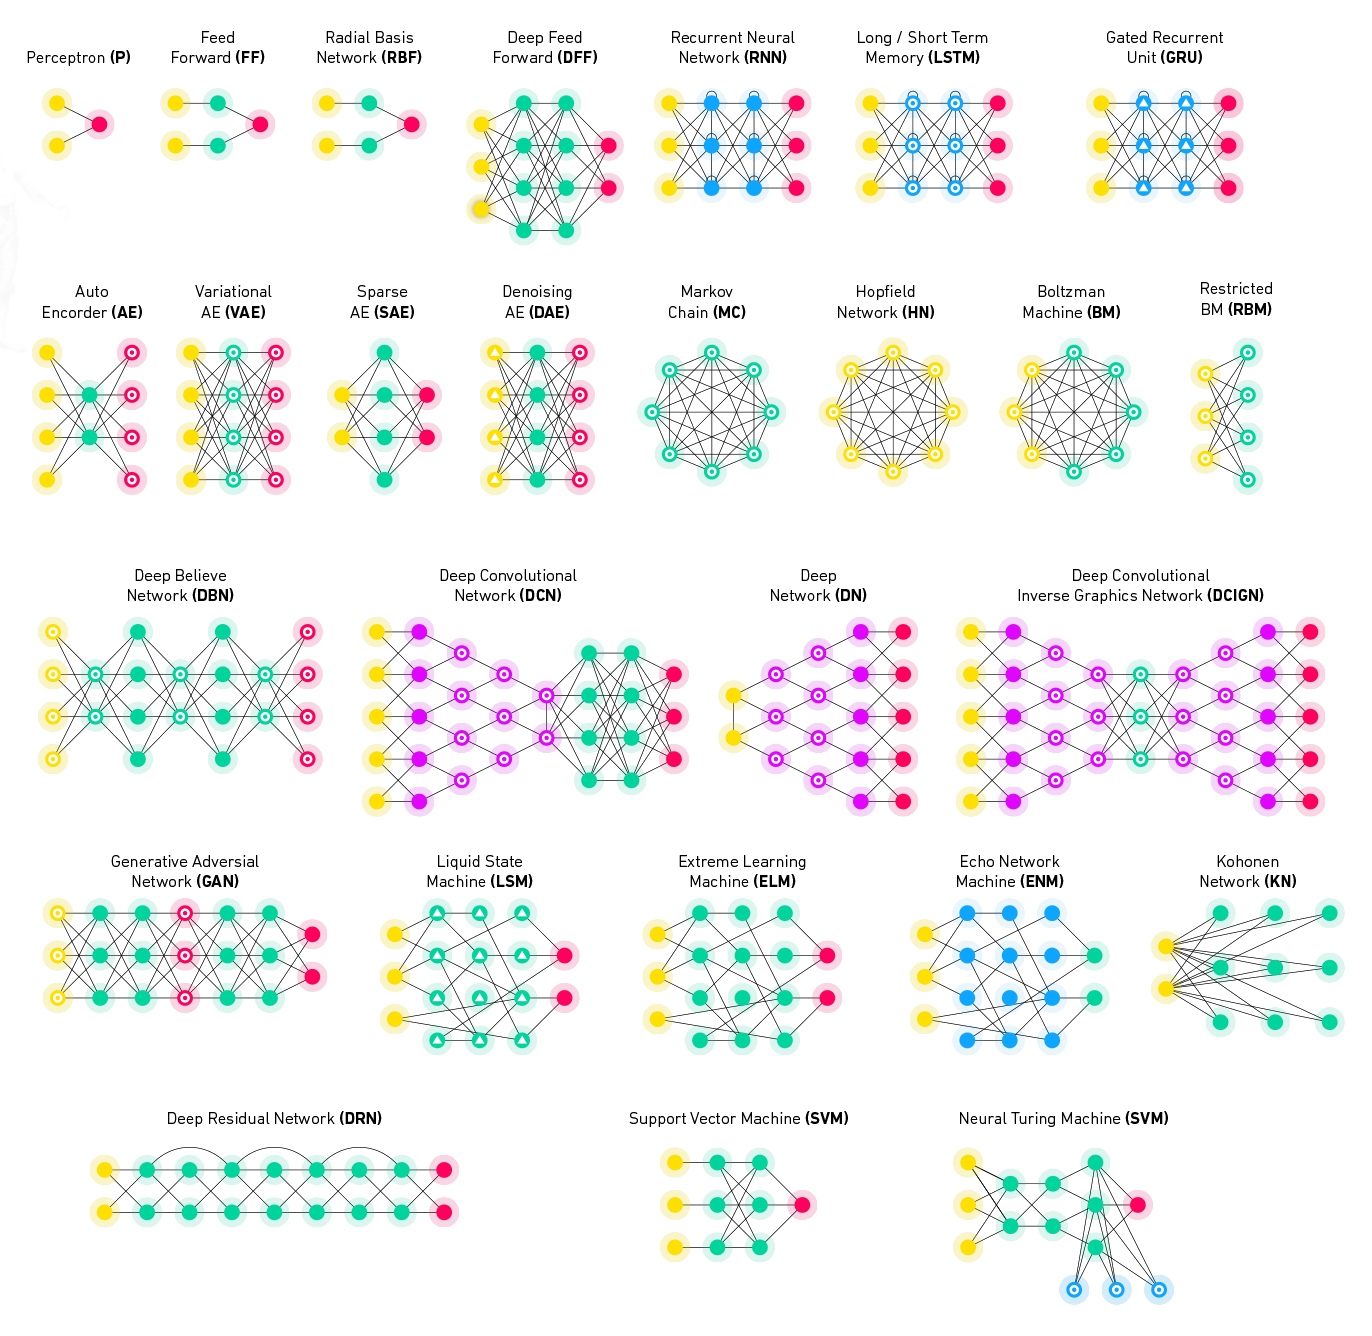
\includegraphics[width=0.8\textwidth]{figures/different_ai_models}
    \caption{Landscape of Modern AI Models and Cloud Providers}
    \label{fig:different_ai_models}
\end{figure}

\subsection{Vector Databases and Embeddings}
To prevent the model from generating plausible but incorrect financial data—a phenomenon known as "hallucination"—the infrastructure integrates Retrieval-Augmented Generation (RAG). RAG utilizes Vector Databases (such as Pinecone or ChromaDB). Documents, accounting standards, and historical client ledgers are converted into high-dimensional vector embeddings. When the AI requires context, the system performs a cosine-similarity search across the vector database to retrieve the mathematically closest factual documents, appending them to the LLM's prompt. This significantly grounds the model's responses in factual reality.

\section{The System Architecture: Multi-Agentic Framework}
While a single LLM prompt can generate text, an audit-ready financial system requires rigorous checks and balances. This dissertation implements a multi-agentic framework using CrewAI. Rather than relying on a monolithic assistant, the architecture decomposes the workload into distinct, specialised roles mimicking a real-world accounting firm.

\begin{enumerate}
    \item \textbf{Senior Financial Analyst (Data Extraction):} This agent operates purely deterministically. Following the "Decimal Mandate," it extracts raw data from the Xero API, refusing to use floating-point arithmetic. It isolates variances greater than 10\% and formats the structured JSON payload.
    \item \textbf{Accounting Partner (Narrative Writer):} This LLM-powered agent receives the deterministic payload and is tasked with synthesizing the human-readable narrative. It is strictly prompted to use the "You" perspective and adhere to statutory narrative sequencing (Turnover, Corporation Tax, Balance Sheet).
    \item \textbf{Quality Control Reviewer (Compliance Assessor):} The final agent reviews the generated text against a strict set of rules (e.g., no explicit journal numbers in the text, verification of numeric matching against the JSON payload). If discrepancies are found, a \textit{ReconciliationError} is raised, and the text is sent back to the Writer for correction.
\end{enumerate}

\subsection{Illustrative Methodology Example}
One representative validation case involves a technology company with unresolved equity movements. In the source working papers, the main issue was whether the year-end note should state a final position on share capital and share premium before the supporting paperwork had been completed. A generic prompting workflow could easily turn the visible movement in equity into a confident summary.

The deterministic layer first identifies investment-related balances and legal or professional-fee activity. The writer agent then drafts a narrative from those facts, while the reviewer agent checks that the wording does not overstate certainty. In the validation corpus, one accountant-authored gold note states that the team is still waiting for investment and share issue confirmation before finalising the share capital and share premium figures. This example shows that accuracy in accounting narrative depends on more than numeric agreement. It also depends on retaining uncertainty where the evidence is incomplete. That point shaped both the fine-tuning dataset and the evaluation rubric used later in the dissertation.

\begin{figure}[H]
    \centering
    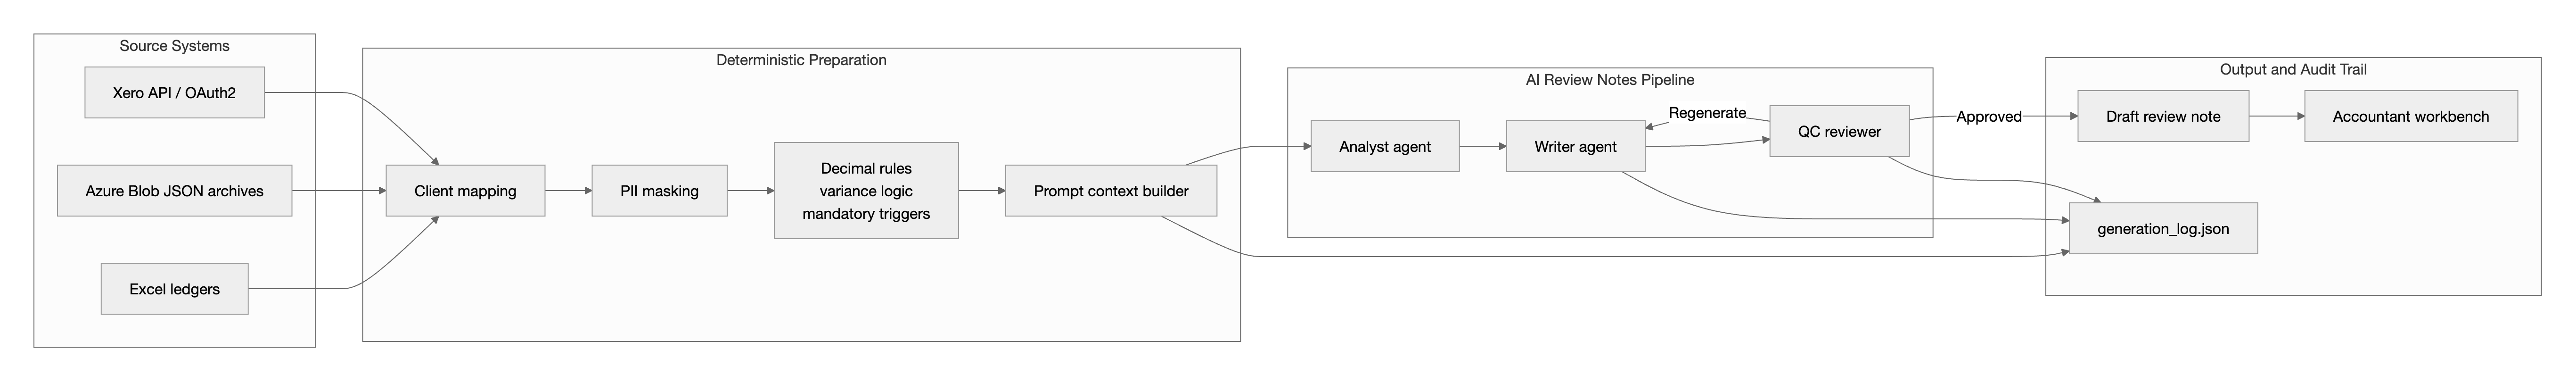
\includegraphics[width=0.92\textwidth]{figures/architecture_diagram}
    \caption{End-to-End System Architecture for the AI Review Notes Pipeline}
    \label{fig:architecture_diagram}
\end{figure}

\section{UX/UI Design and Development}
The effectiveness of an AI-driven system is not solely dependent on its algorithmic performance; the user interface (UI) and user experience (UX) play a critical role in how financial professionals interact with and trust the AI's output. For the PHM UK application, a bespoke design system was developed to ensure clarity, security, and precision.

\subsection{Design Philosophy: Authority, Precision, and Trust}
The design language is anchored in three core pillars:
\begin{itemize}
    \item \textbf{Authority:} A palette of deep navy tones establishes a sense of institutional stability and professional reliability.
    \item \textbf{Precision:} A disciplined 8px grid system and sharp typography (Inter) ensure that dense financial data is presented with mathematical rigor.
    \item \textbf{Trust:} The interface avoids aggressive visual elements, using ambient shadows and high whitespace to focus the accountant's attention on the AI-generated notes and their source data.
\end{itemize}

\subsection{User Journey and Wireframe Development}
To validate the UX, a series of low-fidelity wireframes and high-fidelity interface screens were developed representing the primary accountant journey. The wireframes establish the functional layout, review flow, and feedback loop before the visual layer is applied.

\begin{figure}[H]
    \centering
    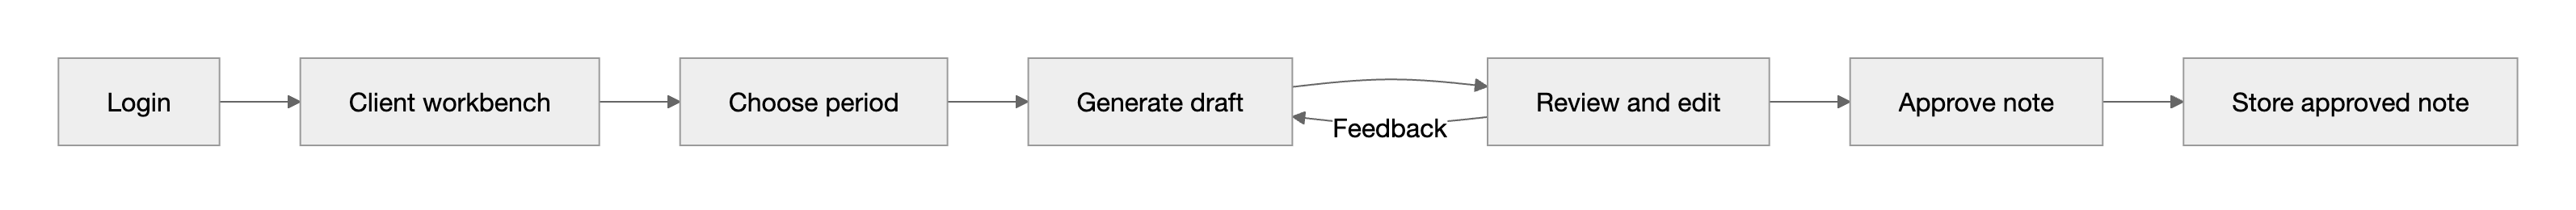
\includegraphics[width=0.88\textwidth]{figures/ui_flow_diagram}
    \caption{Primary User Journey from Authentication to Approved Review Note}
    \label{fig:ui_flow_diagram}
\end{figure}

\begin{figure}[H]
    \centering
    \begin{subfigure}[b]{0.48\textwidth}
        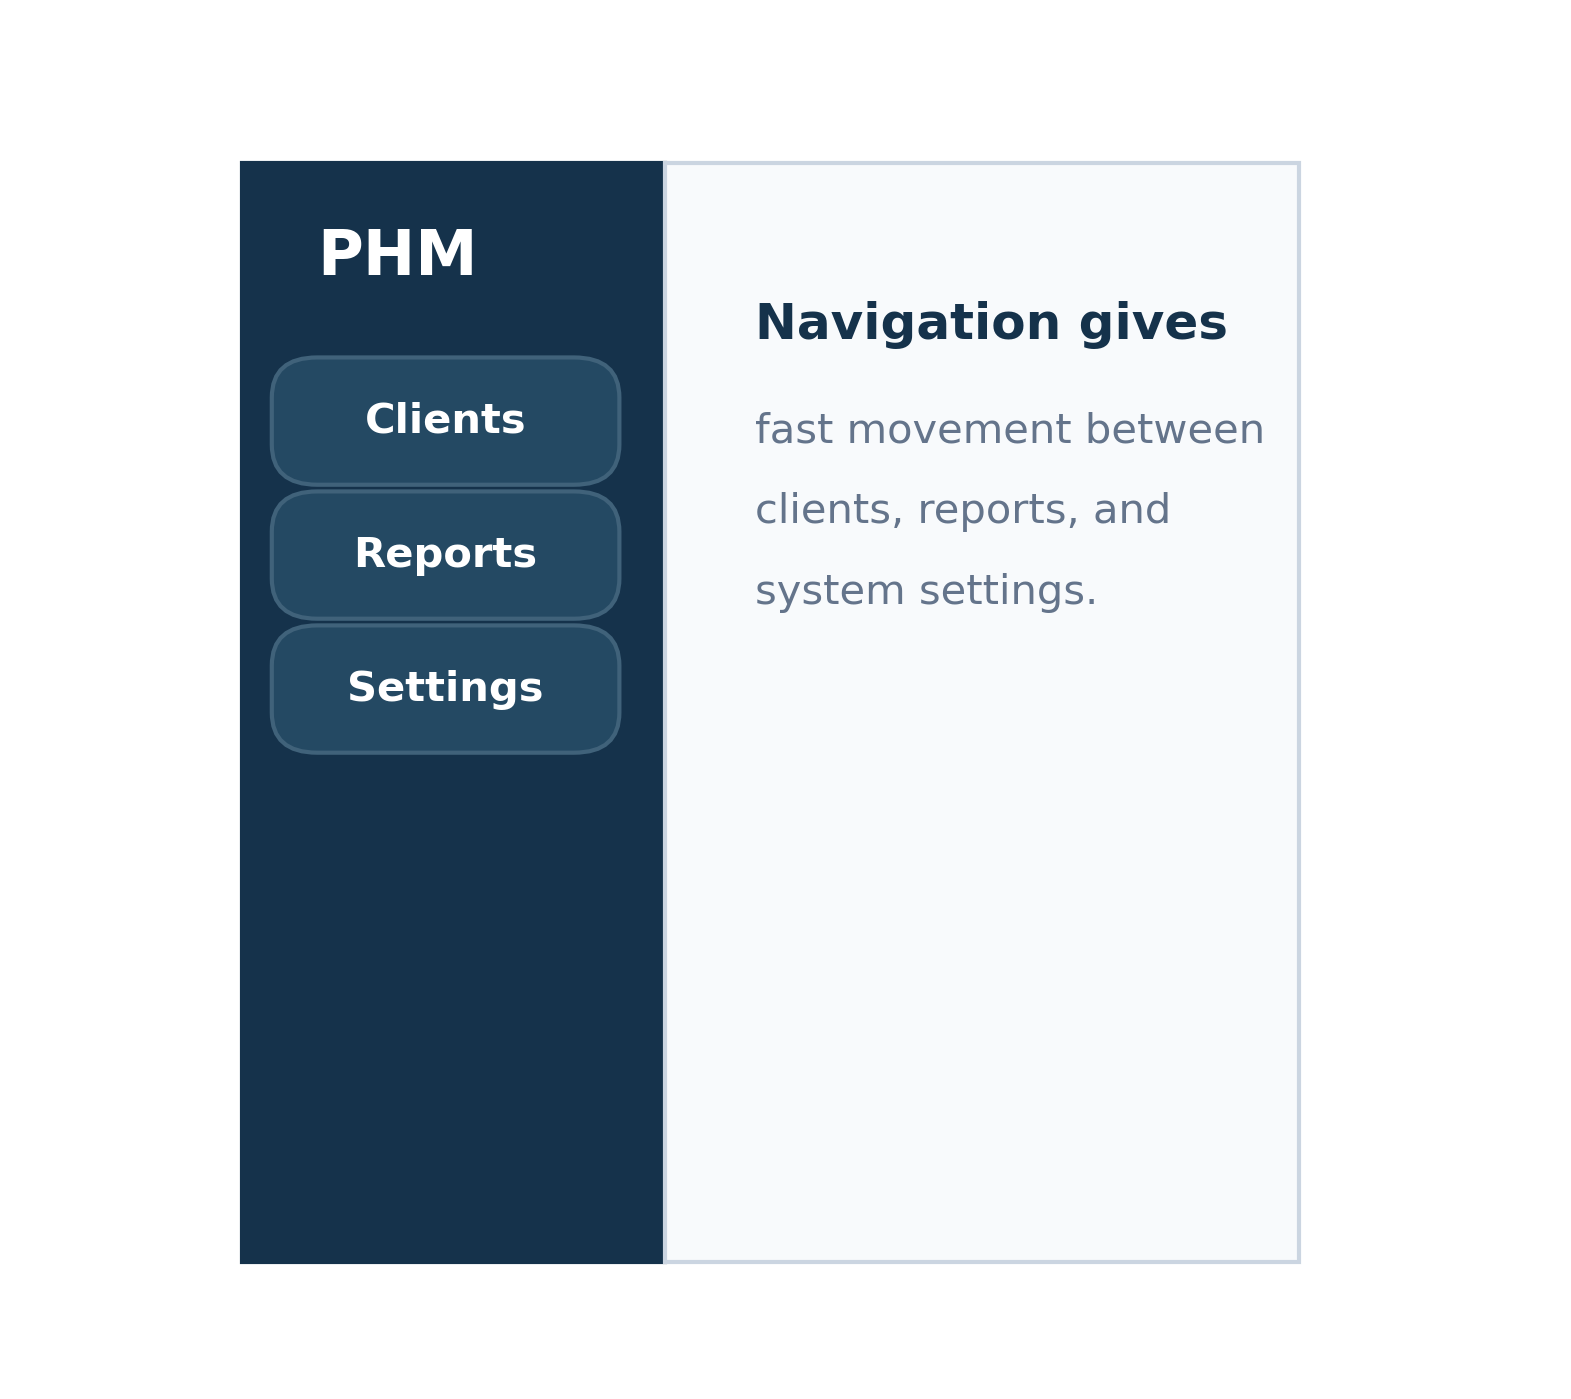
\includegraphics[width=\textwidth]{figures/sidebar_wireframe}
        \caption{Sidebar Navigation Model}
    \end{subfigure}
    \hfill
    \begin{subfigure}[b]{0.48\textwidth}
        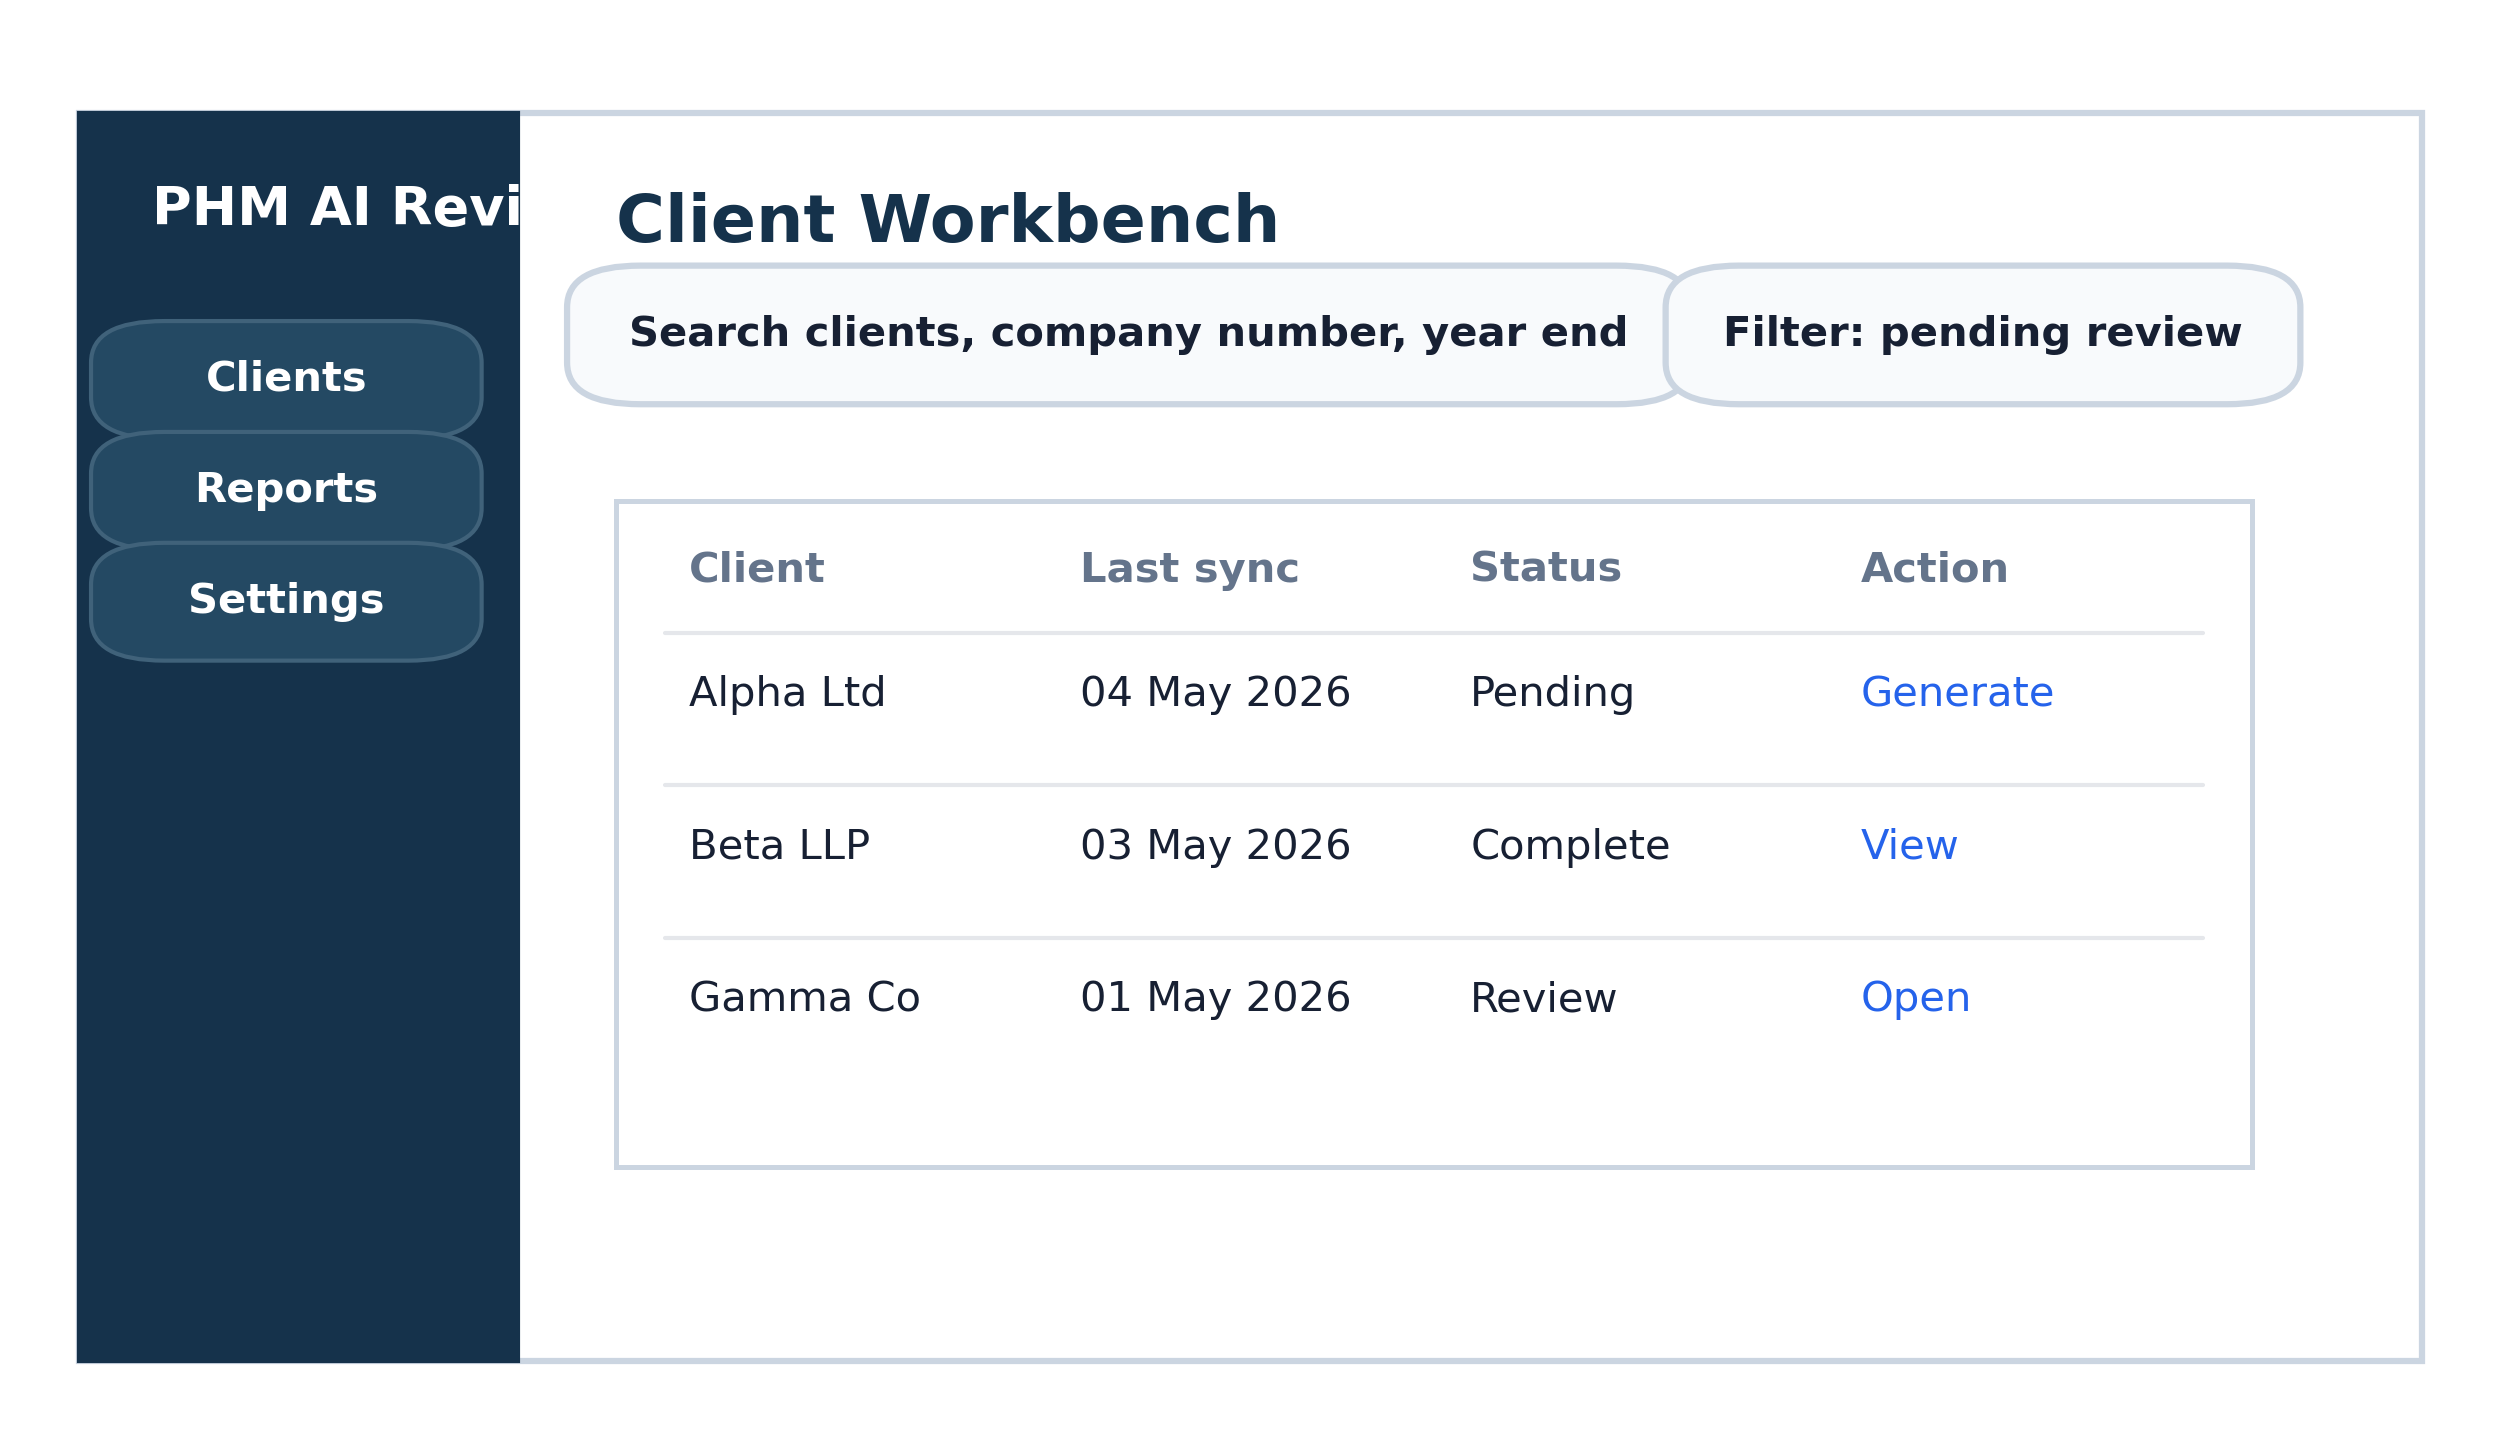
\includegraphics[width=\textwidth]{figures/dashboard_wireframe}
        \caption{Client Workbench Wireframe}
    \end{subfigure}
    \caption{Low-Fidelity Navigation and Dashboard Wireframes}
    \label{fig:navigation_dashboard_wireframes}
\end{figure}

\begin{figure}[H]
    \centering
    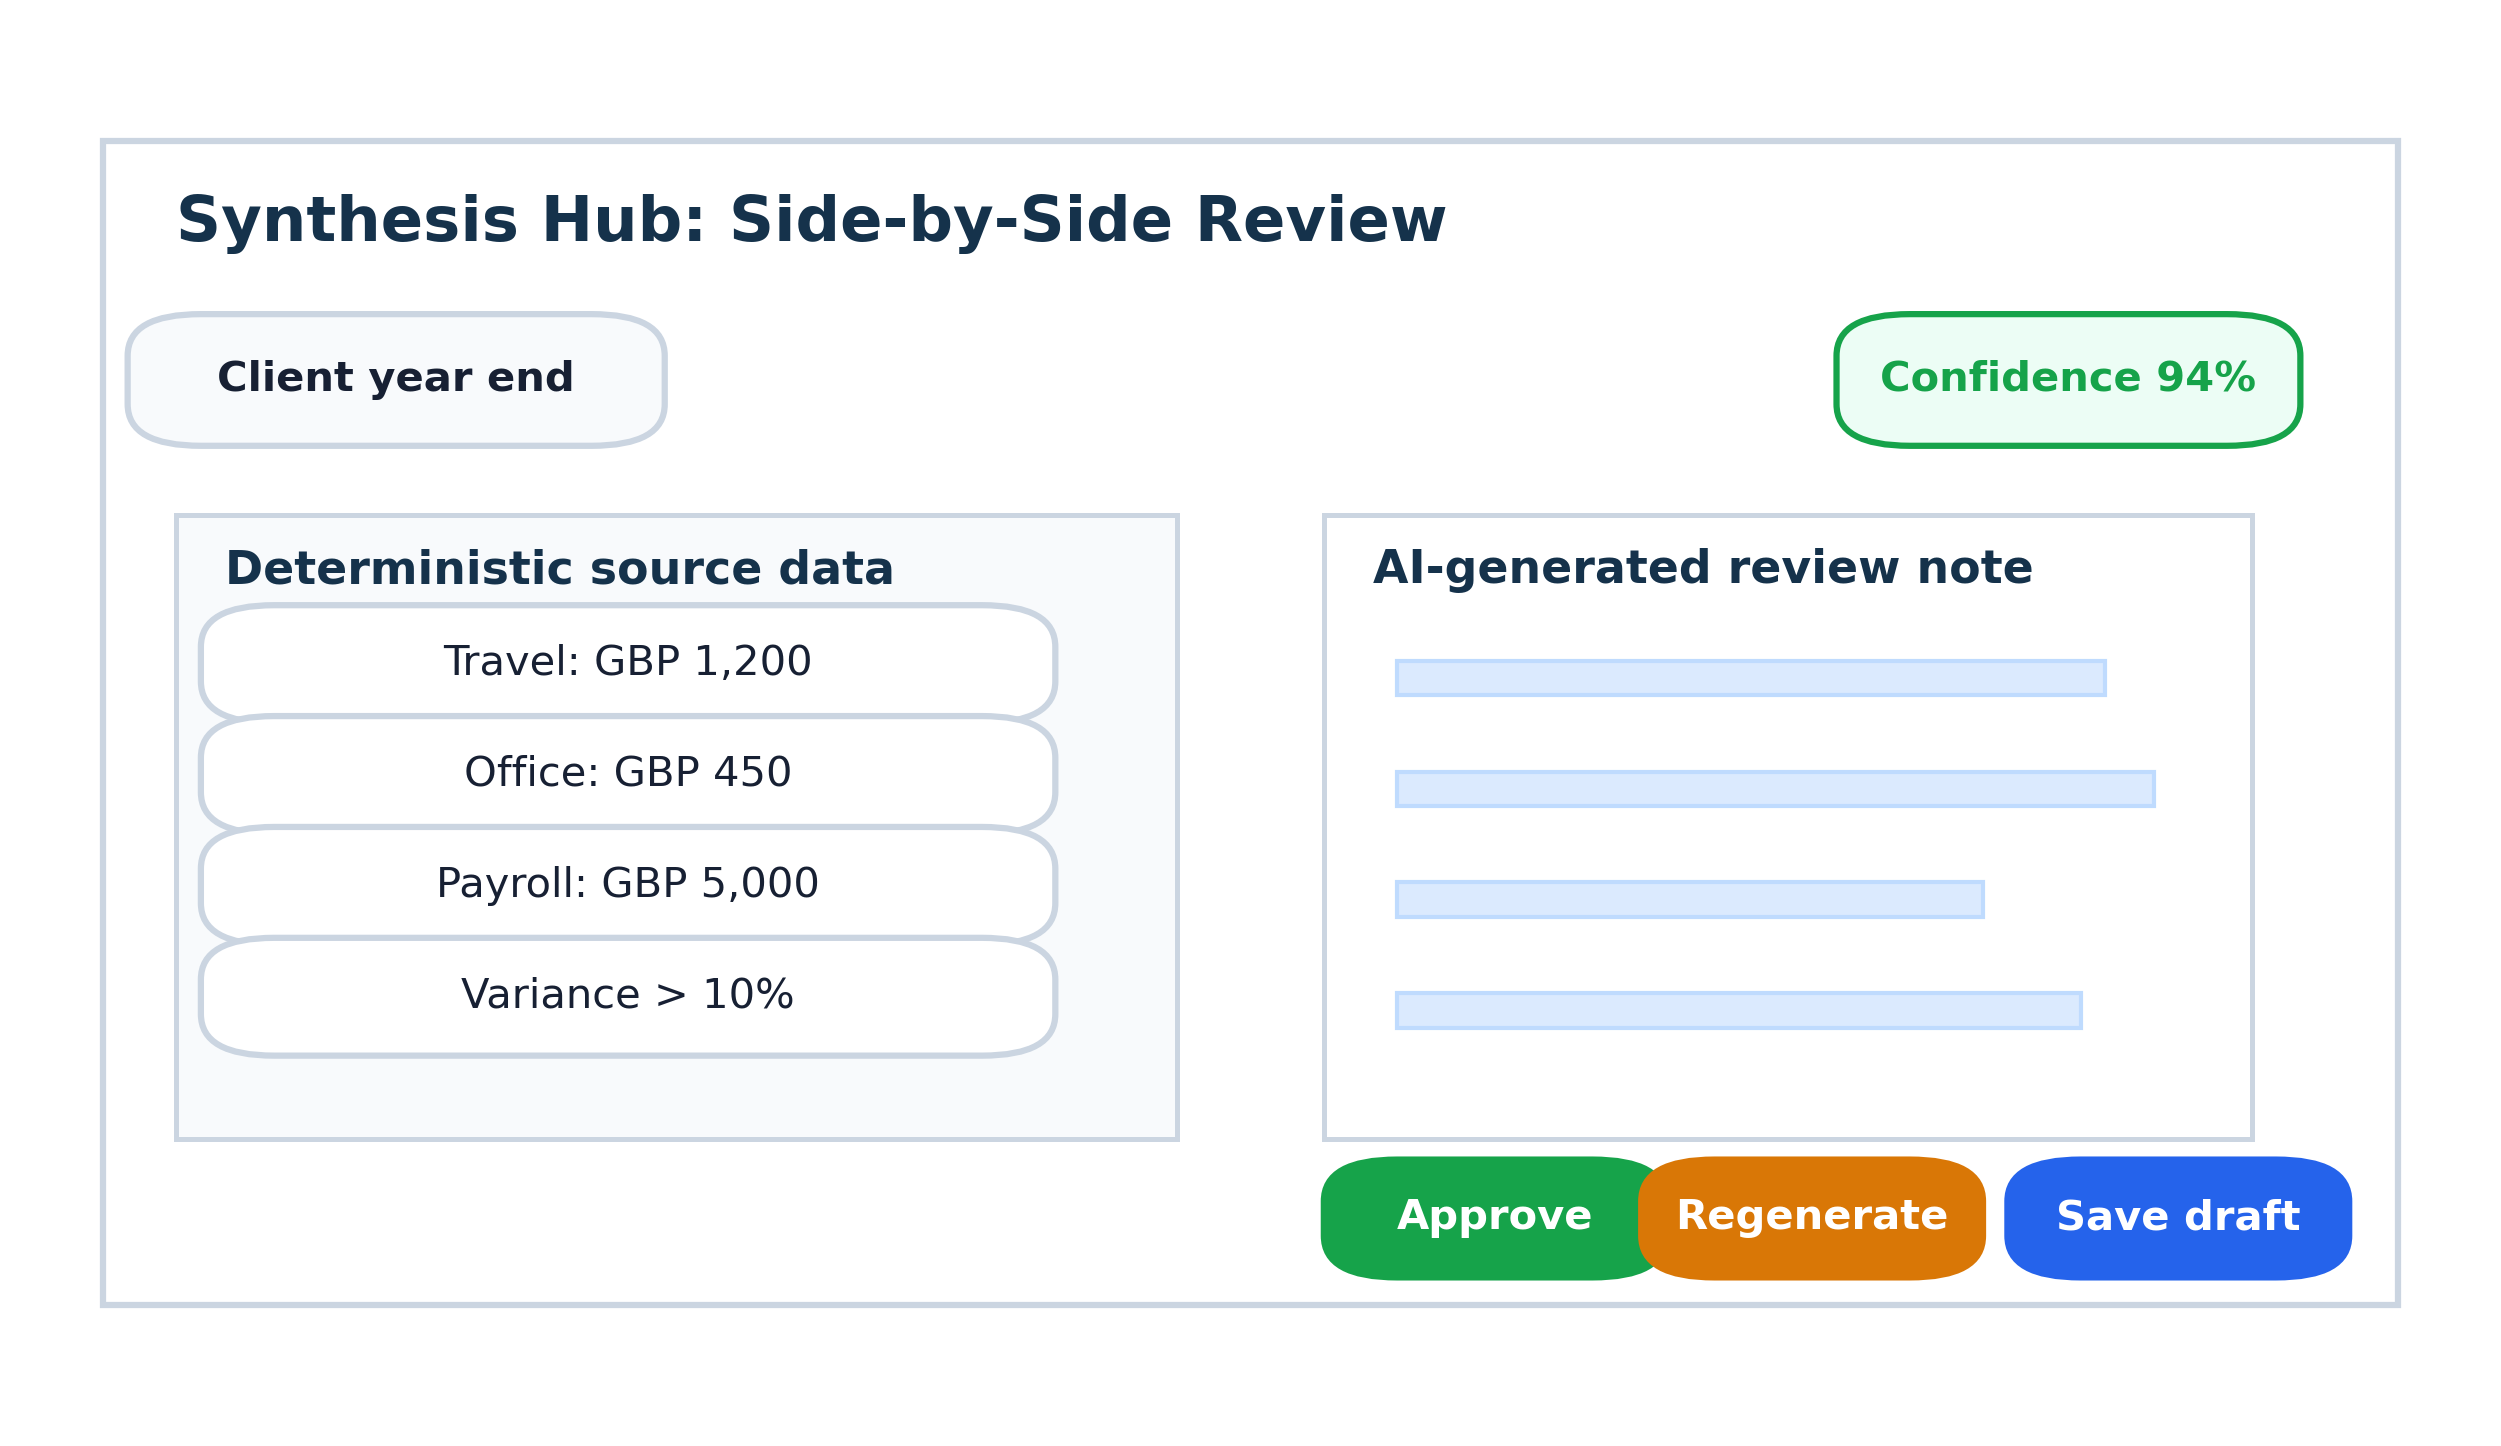
\includegraphics[width=0.9\textwidth]{figures/review_wireframe}
    \caption{Low-Fidelity Side-by-Side Review Wireframe}
    \label{fig:review_wireframe}
\end{figure}

The following high-fidelity screens show the same journey translated into the implemented Flask interface.

\begin{figure}[H]
    \centering
    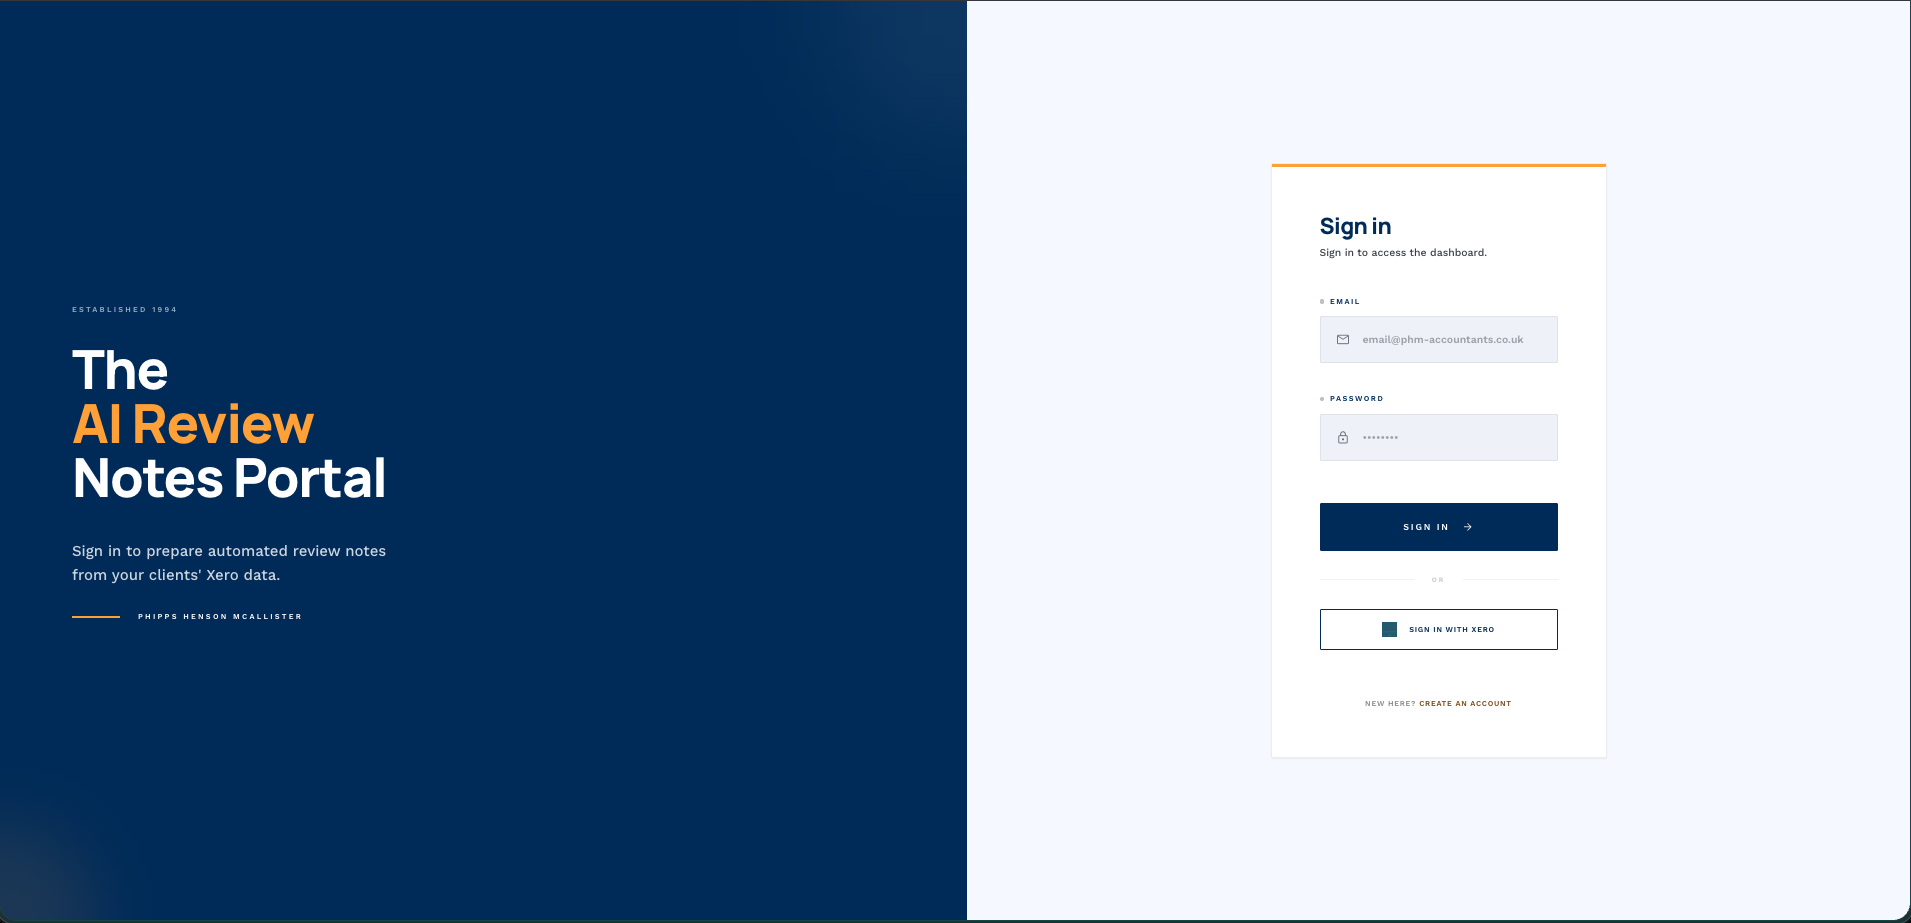
\includegraphics[width=0.7\textwidth]{figures/LOGIN PAGE}
    \caption{User Authentication Interface (Login Page)}
    \label{fig:login_page}
\end{figure}

\begin{figure}[H]
    \centering
    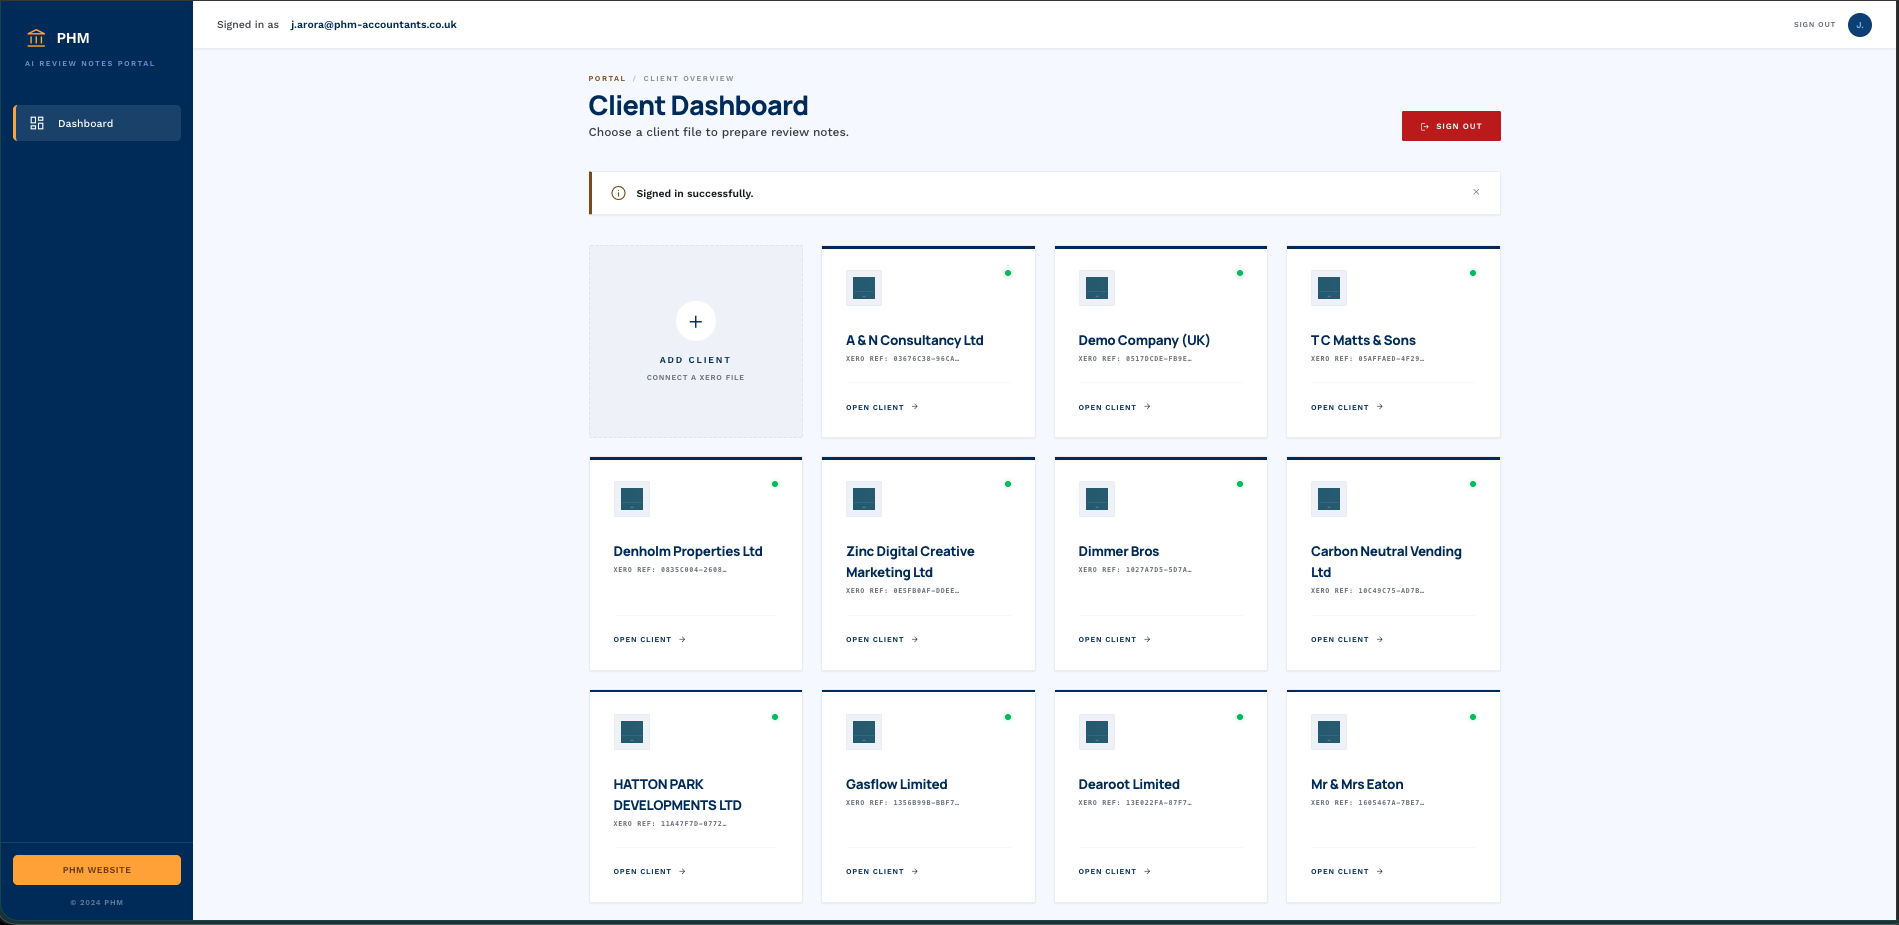
\includegraphics[width=0.9\textwidth]{figures/CLIENTS PAGE}
    \caption{Accountant Workbench: Client Portfolio Overview}
    \label{fig:clients_page}
\end{figure}

\begin{figure}[H]
    \centering
    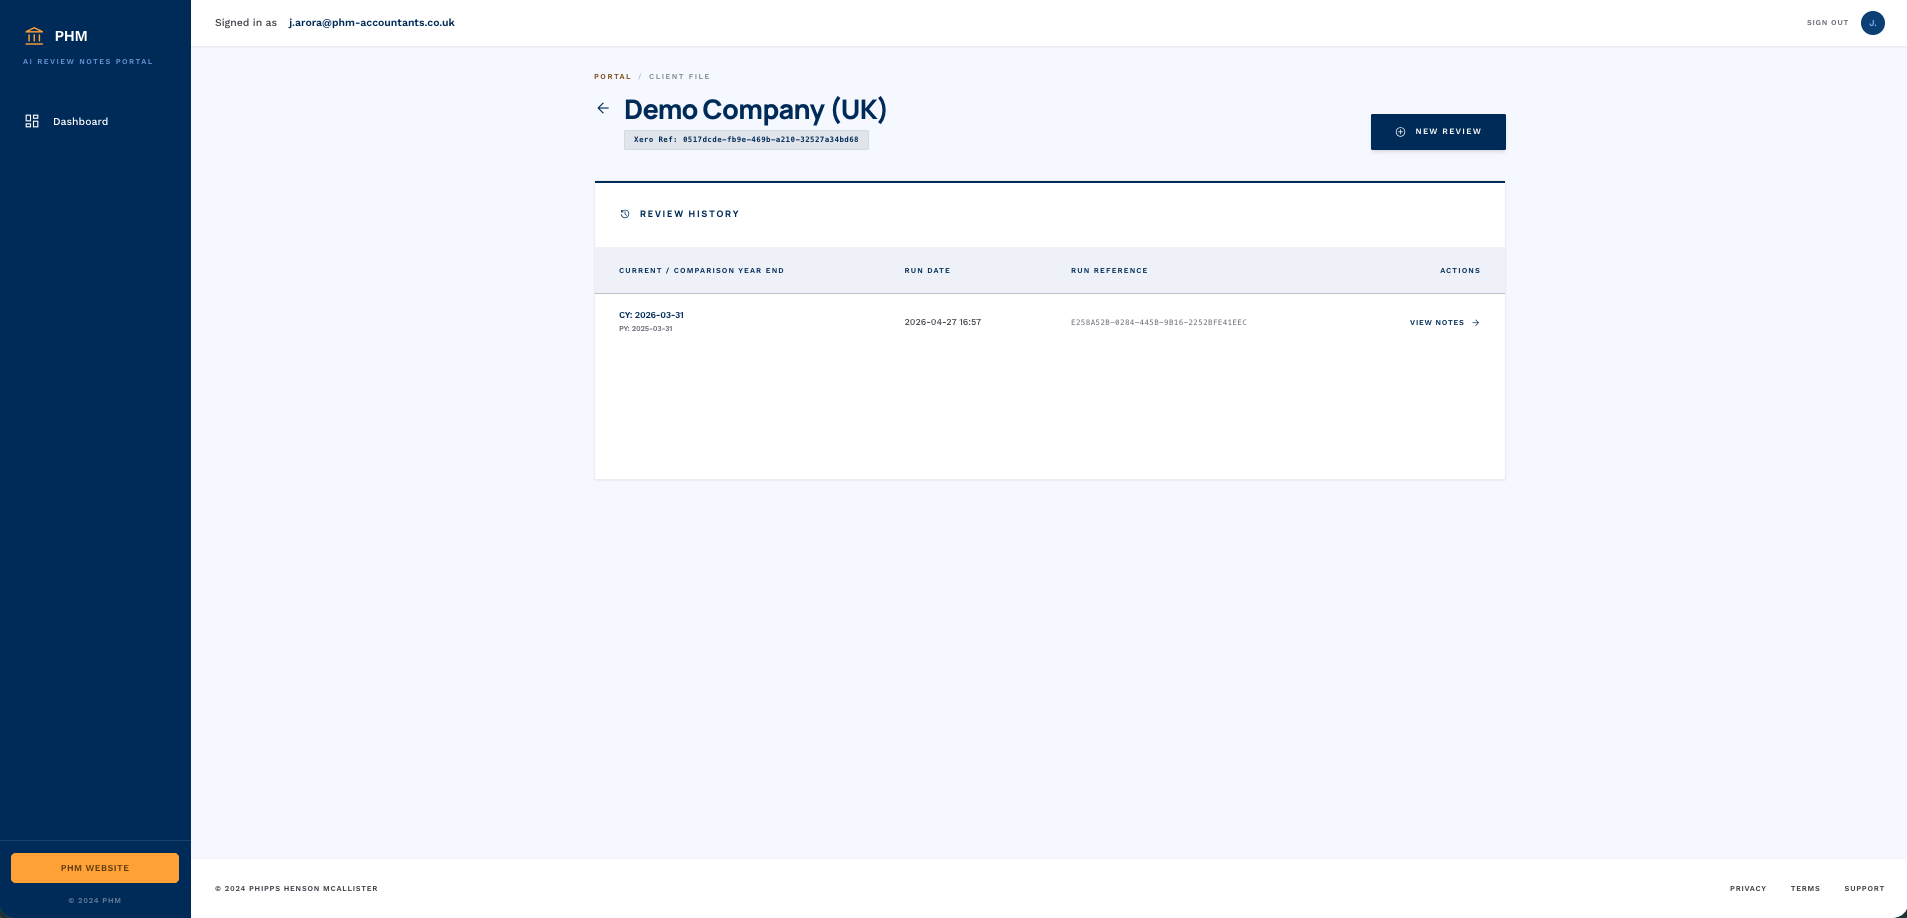
\includegraphics[width=0.9\textwidth]{figures/REPORTS PAGE}
    \caption{Synthesis Hub: Review and Approval Panel}
    \label{fig:reports_page}
\end{figure}

\begin{figure}[H]
    \centering
    \begin{subfigure}[b]{0.45\textwidth}
        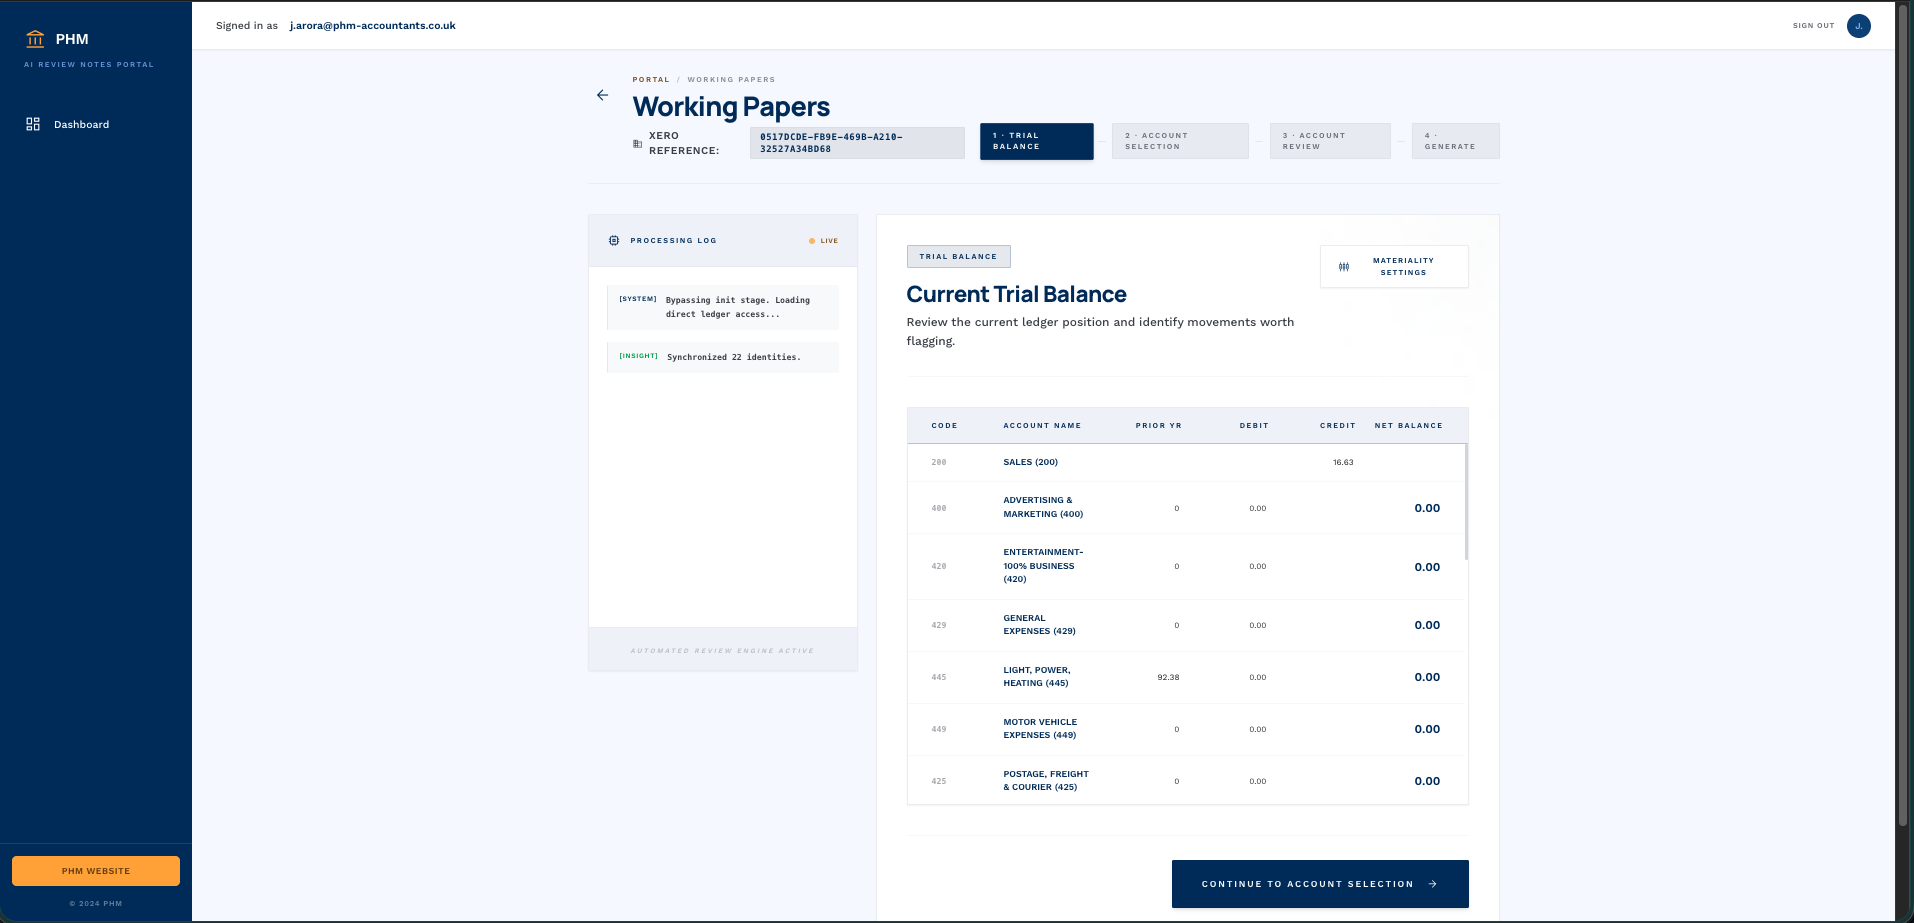
\includegraphics[width=\textwidth]{figures/INIT PAGE}
        \caption{Initial Generation State}
    \end{subfigure}
    \hfill
    \begin{subfigure}[b]{0.45\textwidth}
        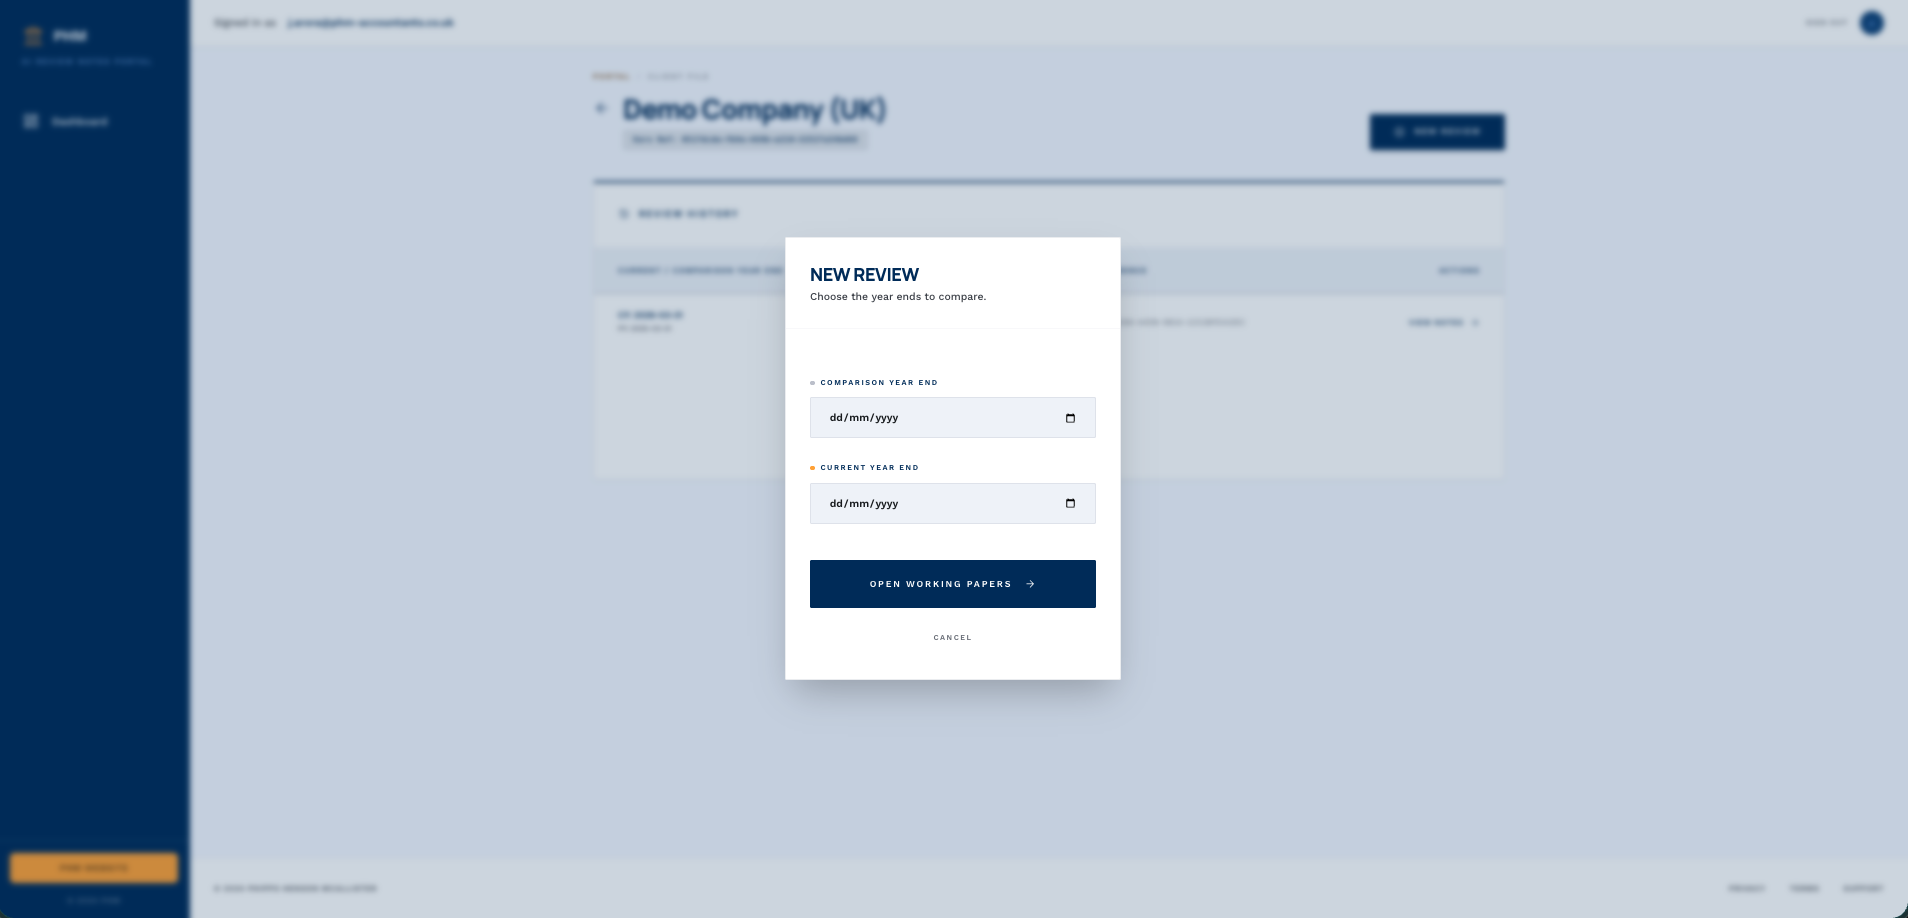
\includegraphics[width=\textwidth]{figures/DATES PAGE}
        \caption{Period Selection Interface}
    \end{subfigure}
    \caption{Supplementary UI Components for Workflow Management}
    \label{fig:supplementary_ui}
\end{figure}

\section{Evaluation Framework: Comparative Analysis of Fine-Tuned Models}
To establish the true capability of modern AI in accounting automation, a comparative evaluation strategy was implemented. Rather than a broad benchmarking of disparate models, this research focuses on the performance of the project's fine-tuned \textbf{GPT-4.1} variants, compared against each other and against the frontier \textbf{GPT-5.4} model using various prompting techniques.

\subsection{Fine-Tuned Model Iterations (GPT-4.1)}
The fine-tuning process was conducted using Azure AI Foundry, specifically targeting the \textbf{GPT-4.1} model---selected for its architectural stability and mature fine-tuning API support. Three distinct fine-tuning recipes were developed using Supervised Fine-Tuning (SFT):
\begin{itemize}
    \item \textbf{FT-A Raw Note SFT:} minimally cleaned historical notes paired with Xero-derived context.
    \item \textbf{FT-B Scrubbed Narrative SFT:} training notes with non-statutory chatter removed so the model learns a tighter accounting narrative.
    \item \textbf{FT-C Scrubbed Plus Rules SFT:} the scrubbed set augmented with deterministic materiality and recurring-subscription cues from the data pipeline.
\end{itemize}

At live benchmark time, the Azure AI Foundry project exposed four callable GPT-4.1 fine-tuned deployments rather than only the three planned recipe labels above. Rather than excluding the extra deployment by hand, all four callable fine-tuned deployments were retained in the measured benchmark so that the comparison reflected the actual project state and did not depend on cherry-picking.

A critical component of this phase was the "Data Scrubbing" pipeline, which was engineered to strip unpredictable human-written narrative (often containing irrelevant "gossip" or non-statutory commentary) from the training corpus. This ensured that the model learned to prioritize mathematical alignment with the Xero Trial Balance over stylistic mimicry of inconsistent human notes.

The training performance was monitored via two primary indicators:
\begin{itemize}
    \item \textbf{Training Loss:} The best run finished with a final train loss of \textbf{1.27}, the second with \textbf{1.36}, and the weakest run with \textbf{1.88}. This spread matters because it shows the fine-tuning process was not uniformly successful across all runs.
    \item \textbf{Mean Token Accuracy:} The corresponding final mean token accuracies were \textbf{0.69}, \textbf{0.67}, and \textbf{0.60}. In practical terms, the first two runs converged into the expected accounting-note range, while the third lagged and later aligned with the weaker behaviours observed in live generation.
\end{itemize}

\begin{figure}[H]
    \centering
    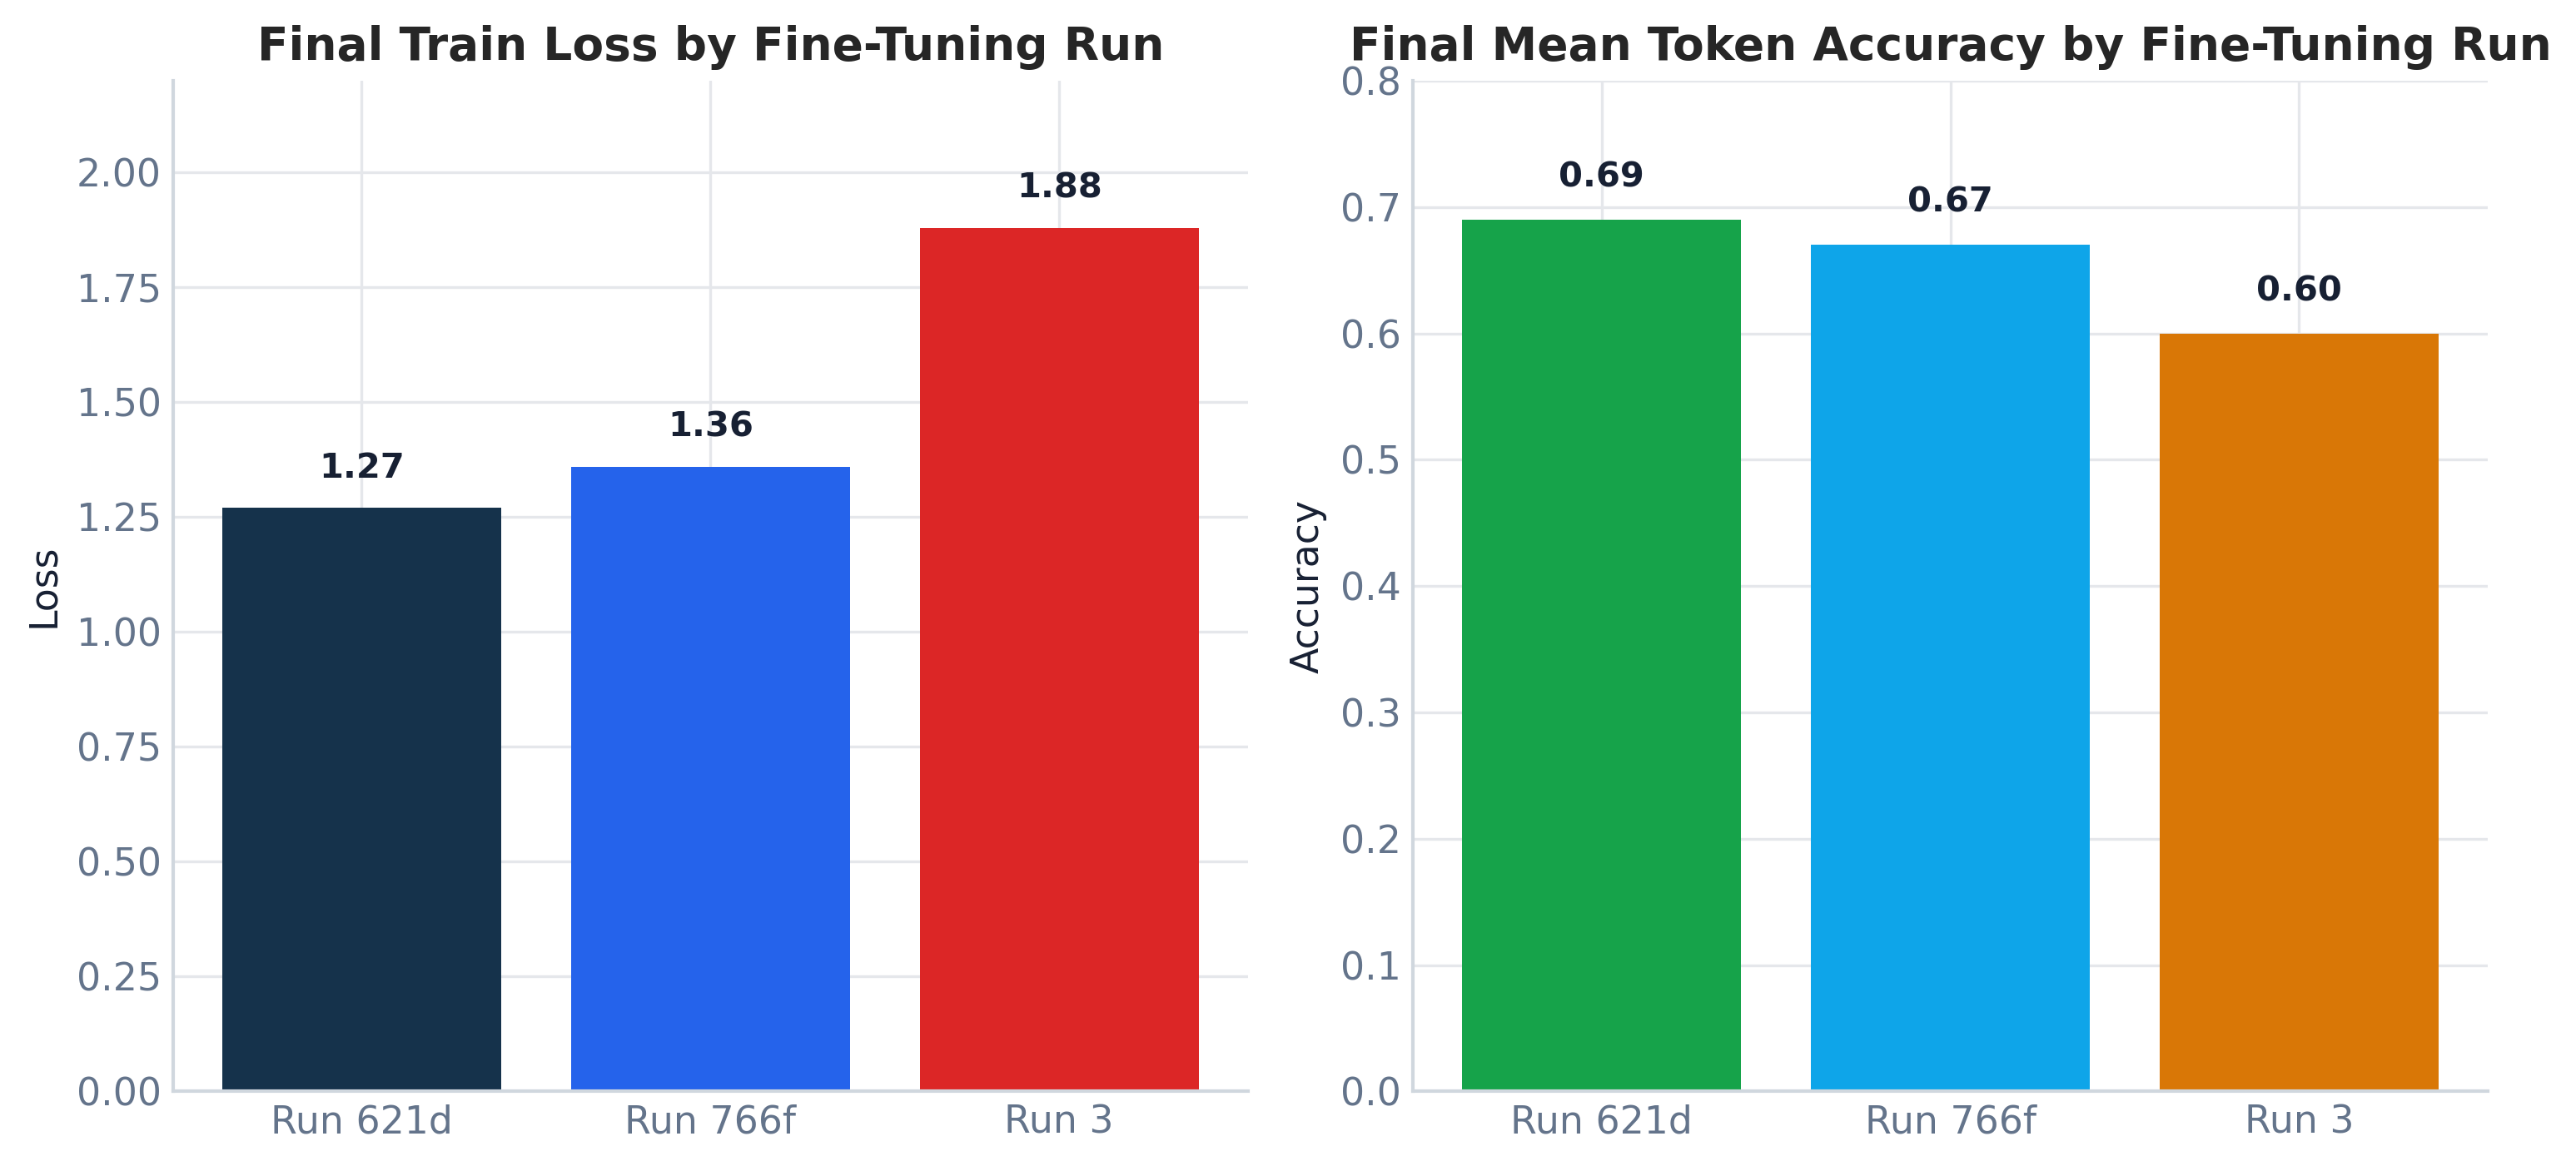
\includegraphics[width=0.9\textwidth]{figures/finetune_run_summary}
    \caption{Final Loss and Mean Token Accuracy Across the Three Main Fine-Tuning Runs}
    \label{fig:training_performance}
\end{figure}

Figure \ref{fig:training_performance} gives the high-level comparison, but the Azure AI Foundry monitor screenshots are also useful because they show the different run shapes directly rather than only the final numbers.

\begin{figure}[H]
    \centering
    \begin{subfigure}[b]{0.32\textwidth}
        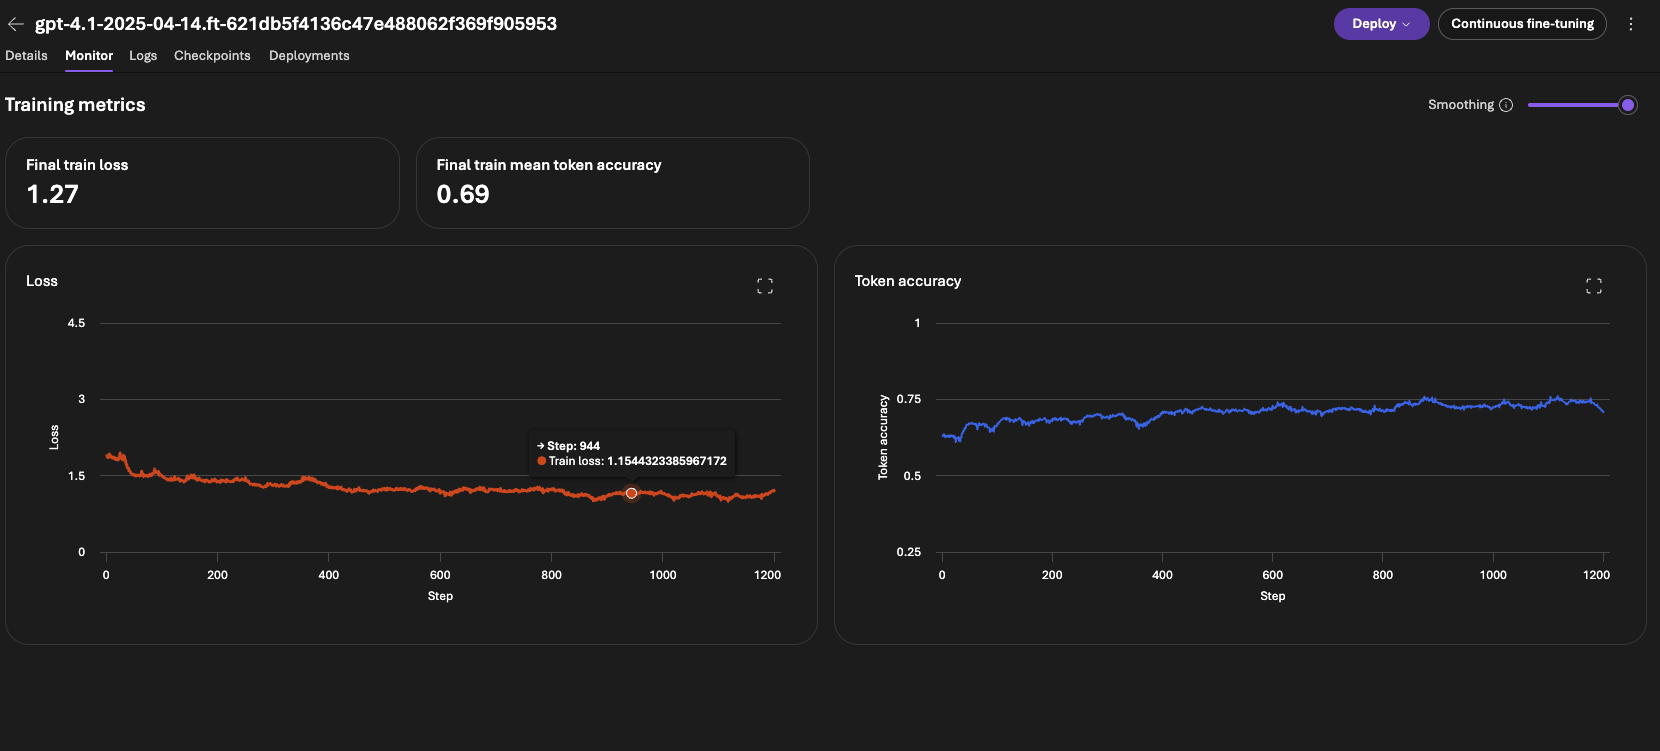
\includegraphics[width=\textwidth]{figures/ft_run_621d_monitor}
        \caption{Run 621d: strongest convergence}
        \label{fig:ft_run_621d_monitor}
    \end{subfigure}
    \hfill
    \begin{subfigure}[b]{0.32\textwidth}
        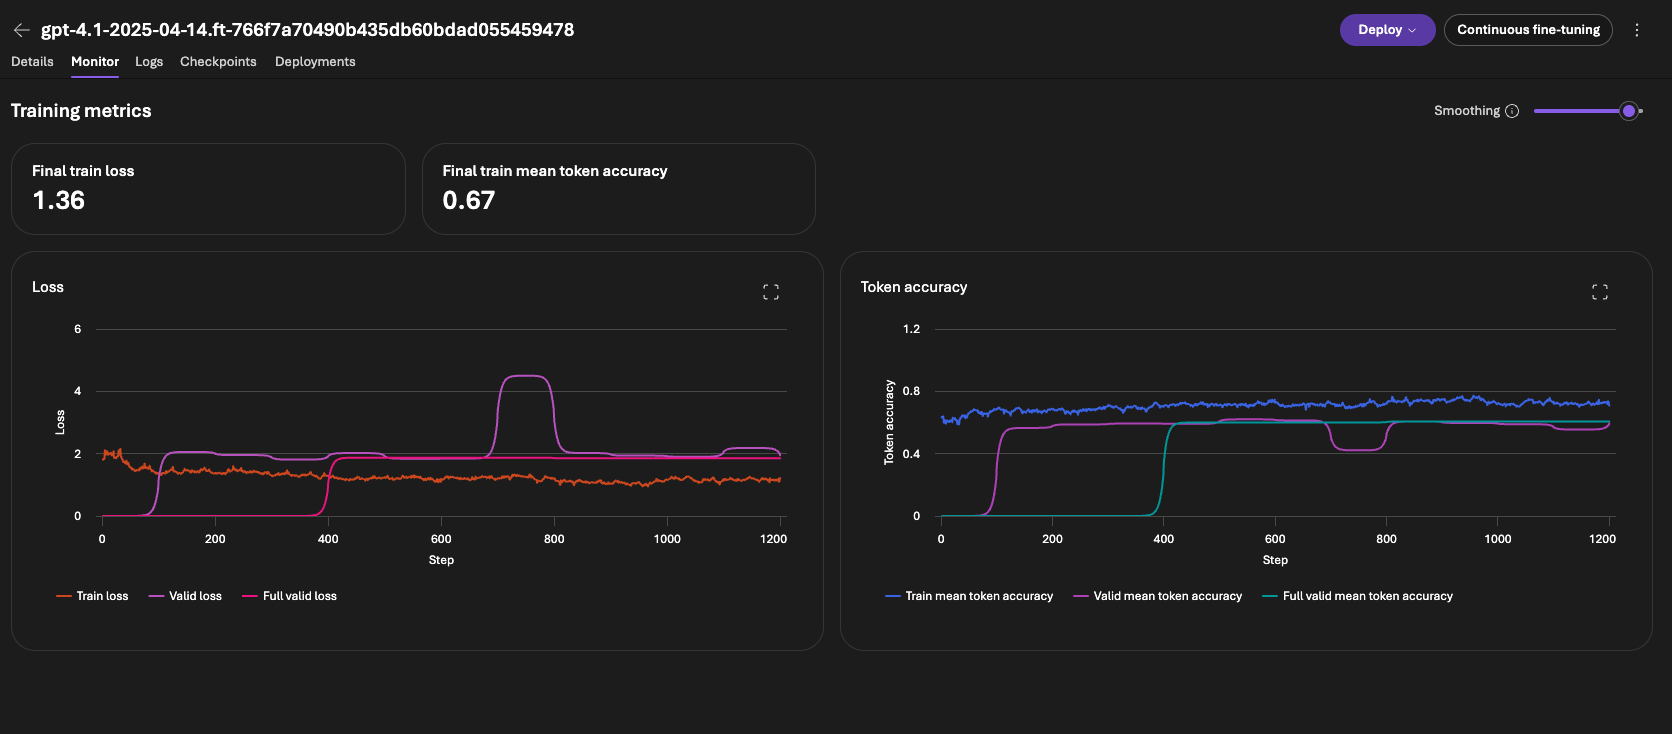
\includegraphics[width=\textwidth]{figures/ft_run_766f_monitor}
        \caption{Run 766f: acceptable but noisier}
        \label{fig:ft_run_766f_monitor}
    \end{subfigure}
    \hfill
    \begin{subfigure}[b]{0.32\textwidth}
        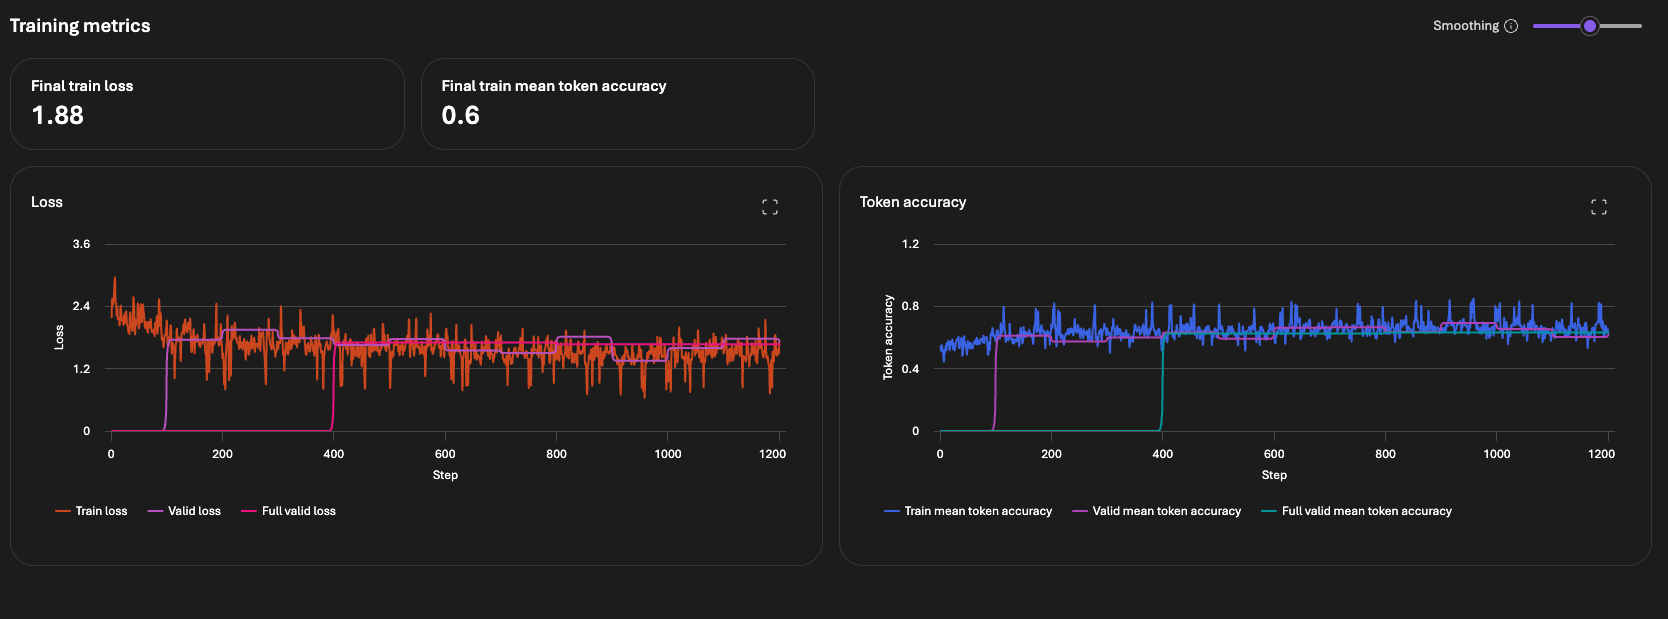
\includegraphics[width=\textwidth]{figures/ft_run_third_monitor}
        \caption{Run 3: weaker convergence}
        \label{fig:ft_run_third_monitor}
    \end{subfigure}
    \caption{Azure AI Foundry Monitor Views for the Three Main Fine-Tuning Runs}
    \label{fig:training_monitor_screens}
\end{figure}

The Foundry monitor views make the quality difference easier to read. The 621d run converged most cleanly and achieved the best final metrics. The 766f run was still usable, but its validation curves were visibly noisier. The third run showed the weakest final loss and token-accuracy values, which is consistent with a poorer checkpoint rather than a mere cosmetic difference in the chart.

These fine-tuned variants are evaluated against each other to identify which training approach best balances narrative precision, numeric fidelity, and reviewer usefulness.


\subsection{Comparative Baseline: Prompt Engineering (GPT-5.4)}
As a high-performance control, the best-performing fine-tuned models are compared against the \textbf{GPT-5.4} model deployed through the Azure AI project endpoint. This baseline model is tested using three primary prompting methodologies to assess whether advanced prompt engineering on a newer model generation can match or exceed the performance of a task-specific fine-tuned predecessor:
\begin{enumerate}
    \item \textbf{Zero-Shot Prompting:} The GPT-5.4 model is given direct instructions without examples.
    \item \textbf{Single-Shot Prompting:} The model is provided with one high-quality example of a standard review note.
    \item \textbf{Few-Shot Prompting:} The model is provided with multiple examples of varying complexity.
\end{enumerate}

The broader validation design uses the 85-record exceptional validation corpus. For the live benchmark reported in this dissertation, a representative three-case subset was executed across the three prompting conditions and all four callable fine-tuned deployments, producing 21 measured generations. The selected cases were chosen to cover a CITB liability adjustment query (\texttt{val\_064}), mixed growth and compliance commentary (\texttt{val\_079}), and unresolved share-issue paperwork (\texttt{val\_084}). Each run was executed with \texttt{temperature=0} and scored against the same accountant-written gold note to isolate the contribution of prompt context from the underlying model capability.

\begin{figure}[H]
    \centering
    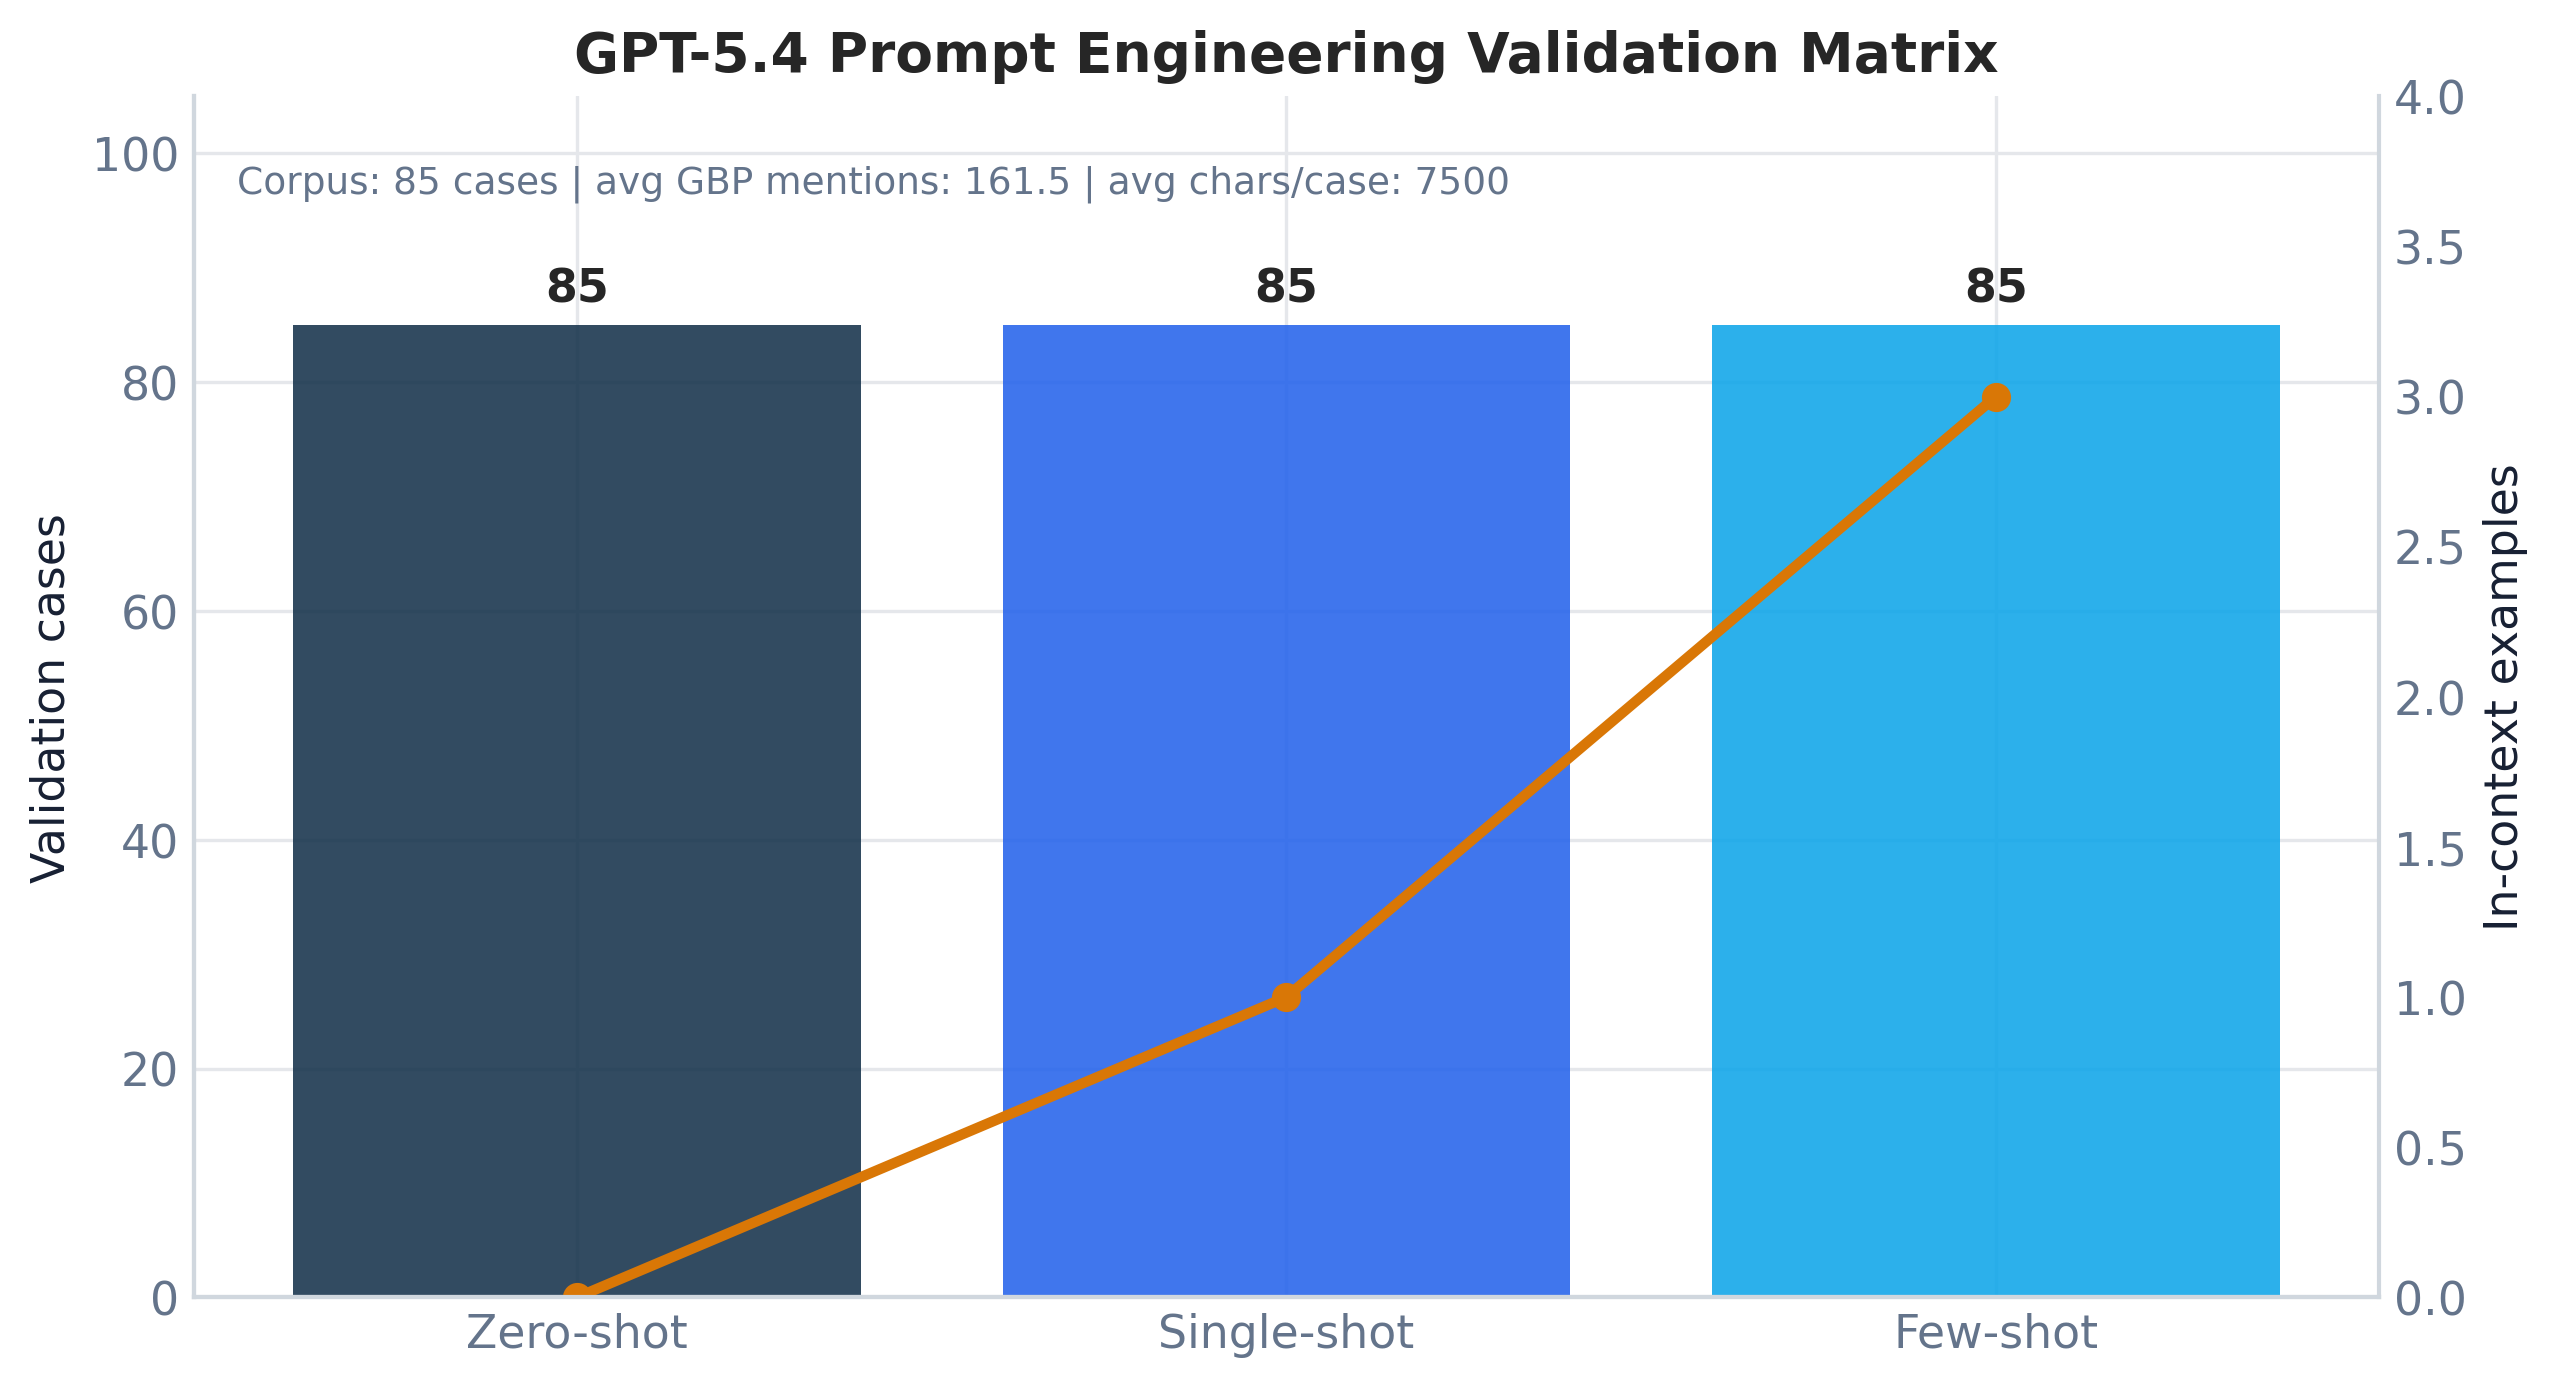
\includegraphics[width=0.82\textwidth]{figures/prompt_engineering_validation_matrix}
    \caption{GPT-5.4 Prompt Engineering Validation Matrix}
    \label{fig:prompt_engineering_validation_matrix}
\end{figure}

The dissertation examples reviewed in the supporting materials do not discuss evaluation only in abstract metric terms. They tie the metric design back to the kinds of cases that matter in professional review. The same approach is used here. The prompt-engineering benchmark is built around long-form accounting cases containing directors' loan accounts, compliance spend, payroll-sensitive commentary, and share issue uncertainty.

\begin{figure}[H]
    \centering
    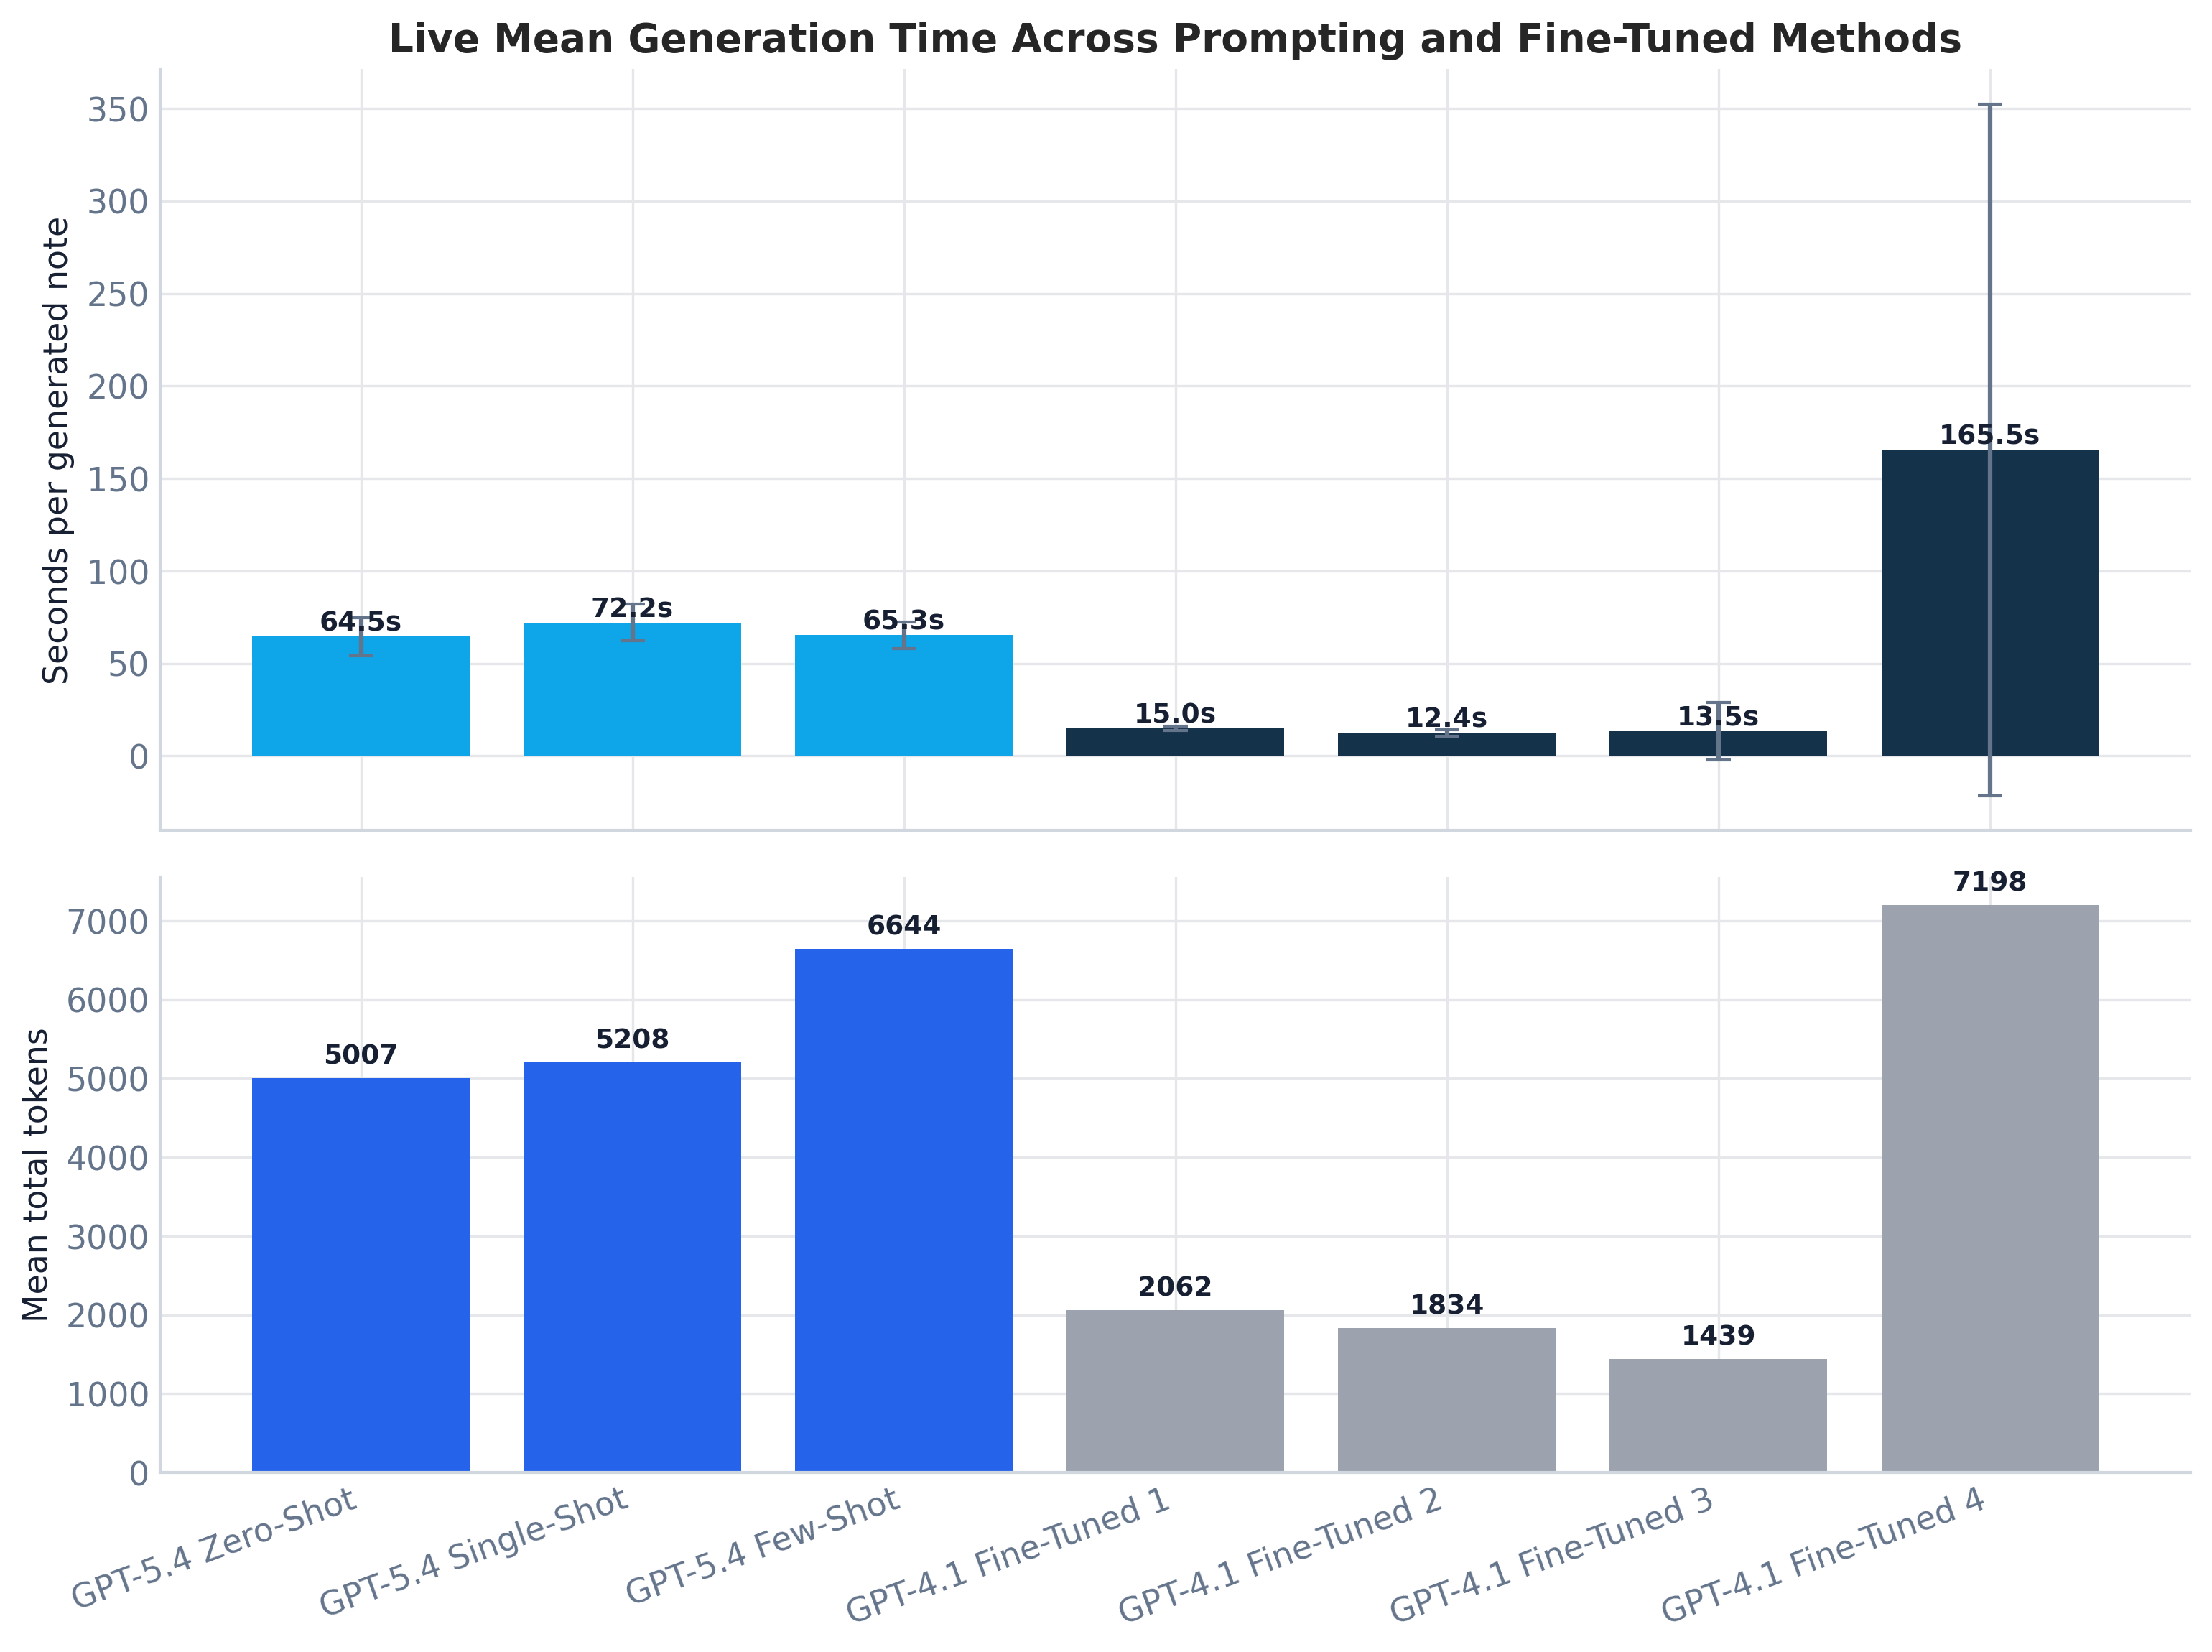
\includegraphics[width=0.9\textwidth]{figures/method_timing_comparison}
    \caption{Measured Time to Produce a Result Across All Tested Methods}
    \label{fig:method_timing_comparison}
\end{figure}

Figure \ref{fig:method_timing_comparison} adds the operational view that the written examples in the context dissertations handled well: the best method is not only the one that writes the cleanest note, but the one that reaches a usable note in a practical amount of time. In the live subset, the prompt-engineering baselines averaged 64.5s (zero-shot), 72.2s (single-shot), and 65.3s (few-shot), while the fastest stable fine-tuned variants averaged 12.4s and 15.0s. The fourth fine-tuned deployment was materially less stable, averaging 165.5s because one case expanded to the output ceiling. That instability is part of the result rather than something to hide.

\subsection{Evaluation Metrics}
All model variations (fine-tuned and prompt-engineered) are tested against four primary criteria:
\begin{itemize}
    \item \textbf{Numeric Fidelity:} Does the generated narrative perfectly match the decimal values extracted from Xero? In financial reporting, a single hallucinated digit constitutes a critical failure.
    \item \textbf{Groundedness and Provenance:} Can the generated statements be traced back to the specific ledger codes provided in the prompt? This measures the system's "Explainability."
    \item \textbf{Narrative Constraints:} Does the model successfully adhere to the firm's strict stylistic rules (e.g., "You" perspective, statutory sequencing, and avoiding redundant journal references)?
    \item \textbf{Time to Produce a Result:} How long each method takes to return a draft note once the case is submitted, together with prompt and completion token usage.
\end{itemize}
The subsequent chapters will detail the specific training datasets used for the fine-tuned models, present the timing profile for all seven tested methods, and compare redacted response examples side by side.

% !TEX root = ../22830110_dissertation.tex

\chapter{Implementation and Development}
\label{chap:implementation}

\section{Technology Stack}
The \textit{ai\_review\_notes} application is designed as a Flask-based web service capable of rapid asynchronous execution. This modern stack was selected to handle the robust requirements of both data engineering and complex NLP tasks.
\begin{itemize}
    \item \textbf{Backend Framework:} Python, Flask, and Celery are used for handling background task processing and enabling real-time UI event emission.
    \item \textbf{Database Architecture:} The application employs SQLite for rapid local development and Azure SQL for production deployment via ODBC normalization, ensuring scalable data storage.
    \item \textbf{AI Orchestration:} The CrewAI framework is used to structure the agents, orchestrating their interaction with Azure OpenAI API endpoints. The fine-tuned configurations were based on GPT-4.1, while the prompt-engineering baseline used the Azure-hosted \texttt{gpt-5.4} deployment.
    \item \textbf{Data Integration:} The Python Xero SDK is deeply integrated for API connectivity, managing token caching securely.
\end{itemize}

Azure is used here for a governance reason as much as a technical one. The system processes sensitive company financial data, and the Azure-hosted model and storage components provide a more appropriate protection boundary for that material than consumer-facing AI tooling. For that reason, the submitted repository intentionally excludes live \texttt{.env} files and active credentials. The code paths are present, but access to live resources is restricted. A working demonstration remains available on request under supervised conditions.

\begin{figure}[H]
    \centering
    \begin{minipage}{0.12\textwidth}
        \centering
        
\includegraphics[width=\textwidth]{figures/flask_logo}
    \end{minipage}\hfill
    \begin{minipage}{0.12\textwidth}
        \centering
        
\includegraphics[width=\textwidth]{figures/celery}
    \end{minipage}\hfill
    \begin{minipage}{0.12\textwidth}
        \centering
        
\includegraphics[width=\textwidth]{figures/azure_sql_logo}
    \end{minipage}\hfill
    \begin{minipage}{0.12\textwidth}
        \centering
        
\includegraphics[width=\textwidth]{figures/xero_logo}
    \end{minipage}\hfill
    \begin{minipage}{0.12\textwidth}
        \centering
        
\includegraphics[width=\textwidth]{figures/crewai_logo}
    \end{minipage}\hfill
    \begin{minipage}{0.12\textwidth}
        \centering
        
\includegraphics[width=\textwidth]{figures/azure_logo}
    \end{minipage}\hfill
    \begin{minipage}{0.12\textwidth}
        \centering
        
\includegraphics[width=\textwidth]{figures/azure_ai_foundry}
    \end{minipage}
    \caption{Core Technology Stack Components}
    \label{fig:tech_stack_logos}
\end{figure}

\section{Data Acquisition and Processing Pipeline}
The foundation of the system is built upon a robust data acquisition and processing pipeline designed to handle heterogeneous client data formats. 

\subsection{Client Identification and Mapping}
The process initiates with data acquisition from raw Excel ledgers provided by the firm. The system extracts the client name from these files and performs a cross-reference mapping against Xero's internal database to securely identify the corresponding \texttt{contact\_id} and \texttt{tenant\_id}. This dynamic mapping bridges the gap between static spreadsheet reports and live cloud accounting environments.

\subsection{Data Fetching and Organisation}
Once the correct Xero tenant is authenticated via the API, the system automatically fetches the complete transaction history, chart of accounts, and ledger data for the specified financial year. The raw JSON payloads retrieved from Xero are often unstructured and overly verbose. The processing engine steps in to systematically organise this data. It filters out irrelevant metadata and categorises transactions into standard accounting classes (Assets, Liabilities, Equity, Revenue, Expenses).

\subsection{Azure Blob and Xero Re-Enrichment Pipeline}
The dissertation dataset was constructed using a two-stage cloud pipeline. First, historical structured working-paper JSON files were loaded from Azure Blob Storage containers containing PHM, Chris, and other client folders. Each file was transformed into a chat-style JSONL record with three components: a system instruction defining the UK accountant role, a user message containing the Xero trial balance and transaction context, and an assistant message containing the target accountant-written review note. The resulting records were split into training and validation JSONL files before upload to Azure AI Foundry for supervised fine-tuning.

Second, lightweight records containing only metadata were re-enriched directly from the Xero API when a valid \texttt{tenant\_id} and year-end date were available. The Xero OAuth2 refresh-token flow was used to maintain access, after which the pipeline fetched reports and transactions for the relevant two-year period. This design ensured that the model was not trained solely on stale spreadsheet exports: where possible, the trial balance and transaction context were reconstructed from live accounting-system data. The implementation also included a connection-gap analysis, matching company names in blob storage against connected Xero tenants to identify clients requiring additional authorisation.

\begin{figure}[H]
    \centering
    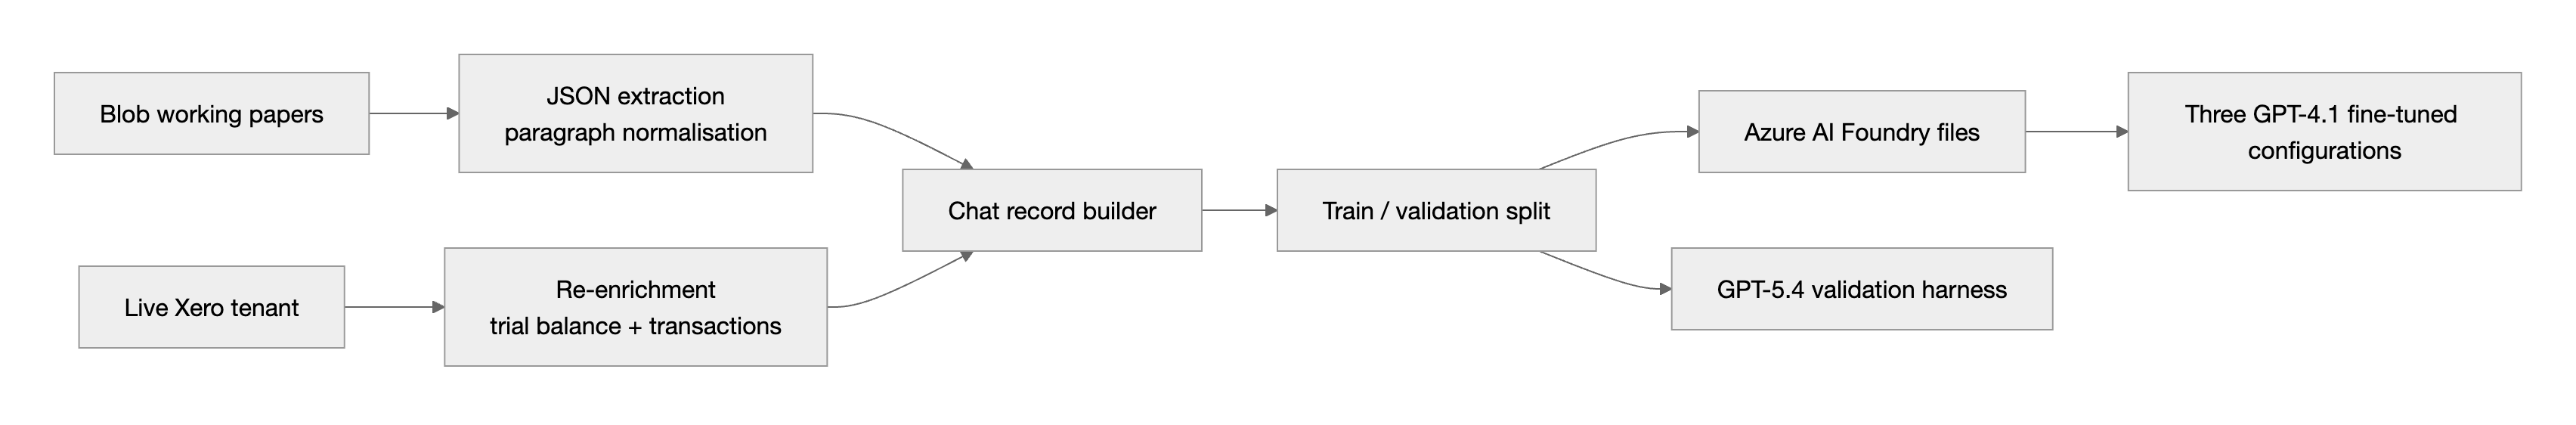
\includegraphics[width=0.92\textwidth]{figures/data_pipeline_lifecycle}
    \caption{Dataset Construction and Validation Lifecycle}
    \label{fig:data_pipeline_lifecycle}
\end{figure}

Figure \ref{fig:data_pipeline_lifecycle} shows the full dataset path. Blob working papers and live Xero re-enrichment feed the same chat-record builder, after which the records are split for fine-tuning and for prompt-engineering validation.

\subsection{Implementation Example: From Raw Balances to a Review Note}
One way to understand the implementation is to follow a real case through the pipeline. One validation example contains large balances for development costs, legal and professional fees, loan interest, investor-related expenditure, and a growing share premium account. At the raw-data level, it appears as a dense trial balance with little narrative structure. The pipeline converts that input into a sequence of machine-usable stages.

First, the ingestion layer preserves the original balances and metadata exactly, without allowing the language model to ``reinterpret'' them numerically. Second, the context builder turns the balance sheet and transaction summaries into a constrained prompt containing the relevant accounting facts. Third, the note-generation harness supplies this context to either a fine-tuned GPT-4.1 model or the GPT-5.4 prompt baseline. The output is not judged only on fluency. It must also preserve the control issue in the source material: further share issue documentation is still required before the final equity position can be treated as complete.

A less constrained prototype could generate a plausible paragraph about investment growth while inventing certainty around shareholdings or paperwork status. The implemented pipeline instead follows the working-paper approach used by the accountants: where the evidence is incomplete, the output should say so directly. That behaviour can be seen in the redacted examples included later in the dissertation.

\subsection{Deterministic Processing and the Decimal Mandate}
Following organisation, the data undergoes deterministic mathematical processing. The system aggregates journal lines and computes variances against prior periods. In strict adherence to the "Decimal Mandate," all calculations are performed using exact decimal arithmetic. The system automatically identifies "material drivers"—variances exceeding the 10\% threshold—and prepares structured summaries, completely isolating the LLM from any mathematical reasoning.

This design matters most in cases involving directors' loan accounts, payroll, or tax liabilities, where even a one-digit drift can change the meaning of the note. For example, a validation case involving overdrawn director balances requires the narrative to preserve the size and reason for the drawings, while distinguishing them from mileage adjustments and dividends. In such a case, letting the model ``do the maths in language'' would add avoidable risk. The implementation therefore treats the LLM as a constrained narrator of pre-computed accounting facts.

\section{Fine-Tuning and Test Environment Construction}
To adapt the general-purpose LLMs to the specific stylistic constraints and reporting formats of PHM UK, an extensive fine-tuning and testing environment was constructed.

\subsection{Model Fine-Tuning}
Historical accounting notes and their corresponding data sets were compiled to create a high-quality training corpus. The system fine-tuned multiple iterations of state-of-the-art models on varying data formats to ensure they internalised the firm's strict "You" persona and paragraph structuring rules. This fine-tuning drastically improved the models' ability to synthesise the deterministic JSON data into professional, audit-ready narrative without hallucination.

\subsection{Test Environment}
The \texttt{experiments/} module serves as a local test environment. It isolates the scoring mechanisms and model benchmarking protocols from the main web application. The final live benchmark harness (\path{experiments/benchmark_dissertation_methods.py}) automates the execution of zero-shot, single-shot, and few-shot prompts against the \texttt{gpt-5.4} Azure deployment and all four callable GPT-4.1 fine-tuned deployments discovered in the Foundry project, tracking numeric fidelity, token usage, and execution time. The harness reads credentials from environment variables only and writes model outputs to a local CSV for later scoring, avoiding the storage of secrets in source code or dissertation artefacts. This is why the submitted repository includes the benchmark code but not the live environment configuration itself.

This test environment was used to check more than readable prose. It was used on cases that appear in real firm workpapers: compliance-related spend described under staff training, legal fees added back for corporation tax, unresolved equity paperwork, and commentary around directors' drawings.

\section{Core Modules and Directory Structure}
The system's logic is modularised to maintain the separation of concerns, dividing the deterministic rules from the stochastic AI generation:
\begin{itemize}
    \item \textbf{App \& Routing (\texttt{app.py}):} The entry point defining the web routes and integrating the CrewAI kickoff process.
    \item \textbf{Agent Definitions (\texttt{agents/crew\_manager.py}):} This file defines the roles, backstories, and goals for the three primary agents: the Financial Analyst, the Writer, and the Reviewer.
    \item \textbf{Data Processing (\texttt{helpers/}):} Contains the Xero API parsers, data masking utilities, and deterministic mathematical rules enforcing the Decimal Mandate.
    \item \textbf{Experiments (\texttt{experiments/}):} A dedicated module for LLM benchmarking and scoring.
\end{itemize}

\section{Provenance and Traceability Implementation}
A core requirement for any accounting software is auditability. To achieve this, every numeric output generated by the system includes either a \texttt{source\_journal\_id} or a \texttt{ledger\_account\_code}. The system automatically generates a \texttt{generation\_log.json} for each session. This log acts as a comprehensive audit trail that snapshots model parameters, prompt templates, and raw input data, ensuring the system remains ``Explainable by Design'' at all times.

\begin{figure}[H]
    \centering
    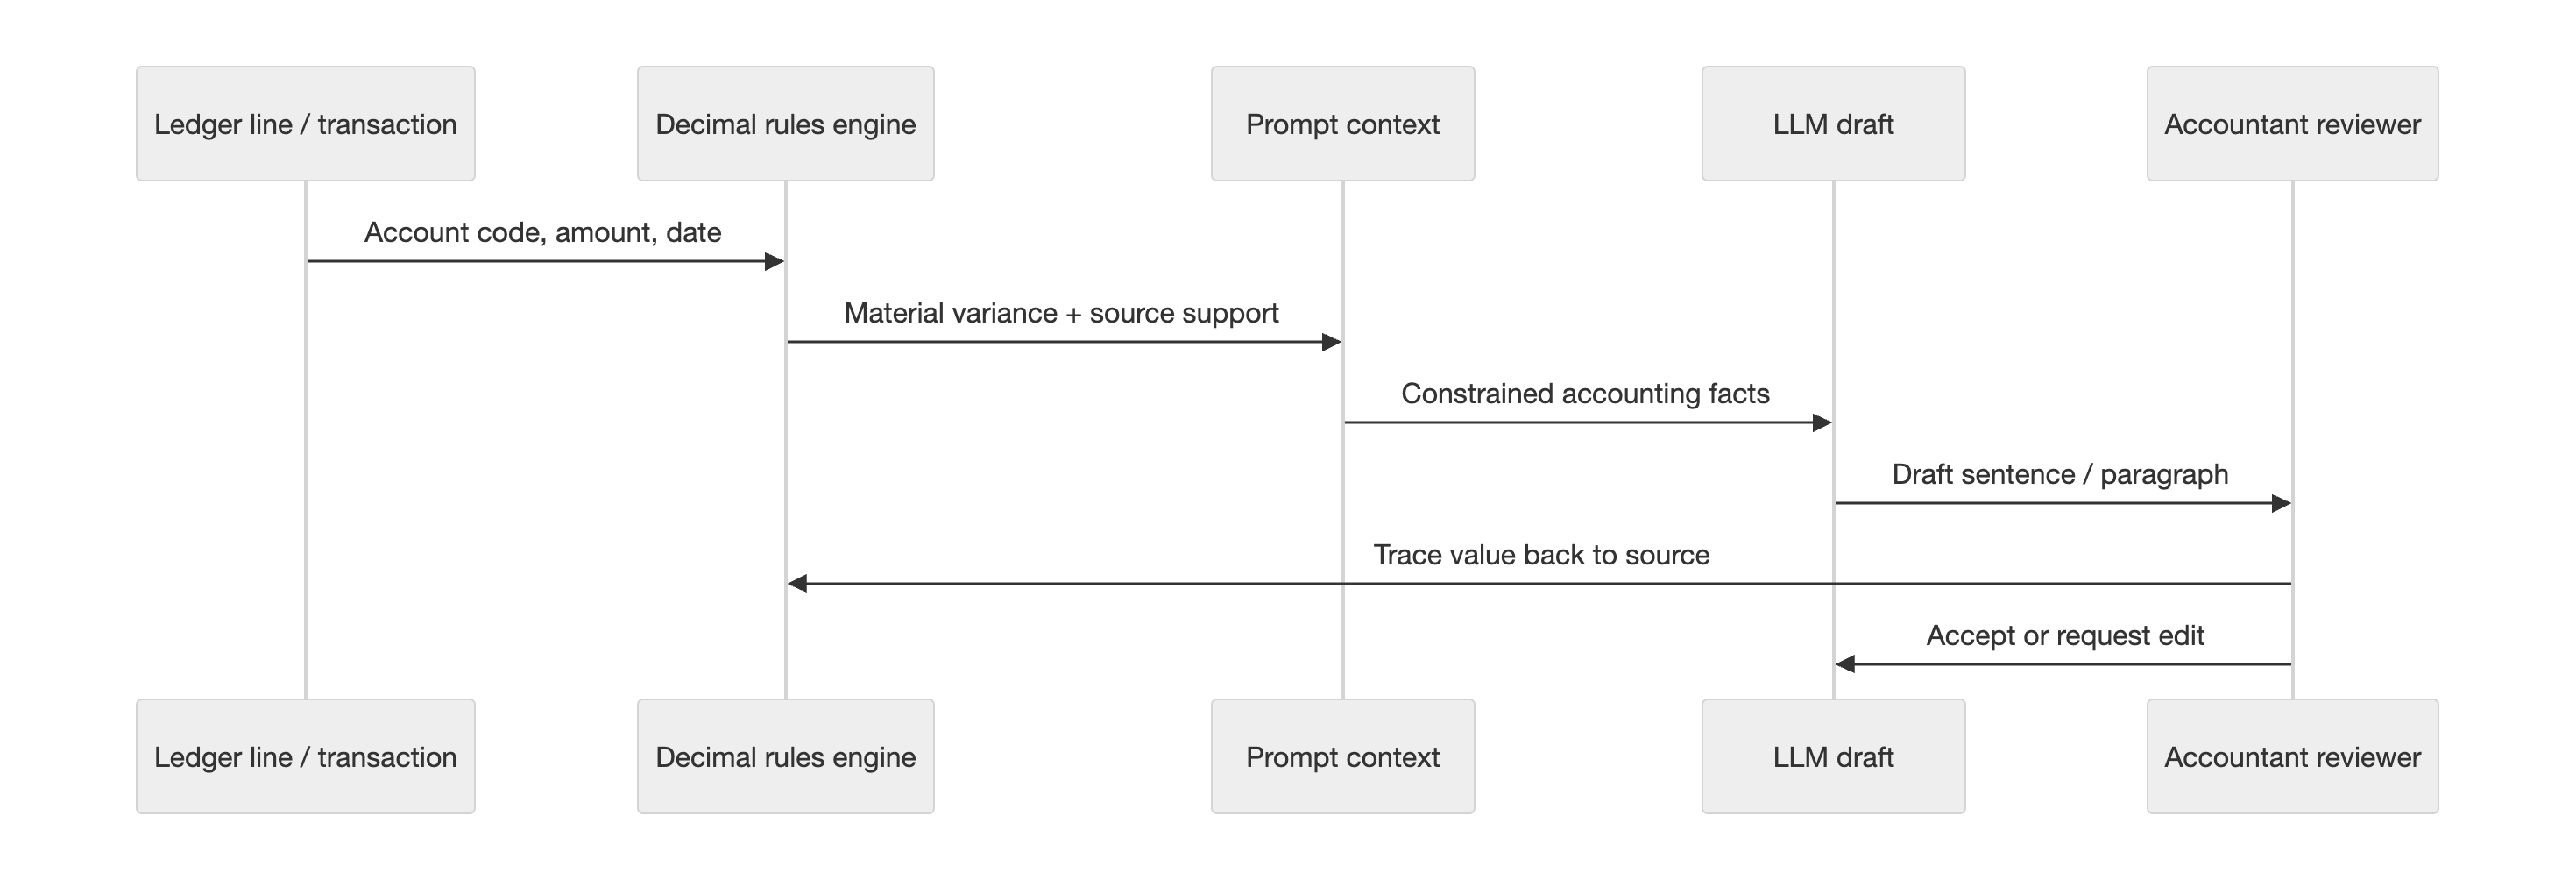
\includegraphics[width=0.88\textwidth]{figures/provenance_trace}
    \caption{Trace from Ledger Evidence to Reviewer Verification}
    \label{fig:provenance_trace}
\end{figure}

Figure \ref{fig:provenance_trace} reduces provenance to the steps that matter during review. A transaction or ledger line is carried through the deterministic engine into the prompt context, then into the draft note, and can be checked again by the reviewer when a figure or claim needs support.

\section{UI/UX Technical Implementation}
The front-end of the application was implemented using Flask's Jinja2 templating engine combined with modern CSS Grid and Flexbox layouts. The primary design goal was to translate the "Accountant Workbench" wireframes into a functional, high-performance interface.

\subsection{Side-by-Side Review Interface}
The main UI component is the \textit{Review Panel}, implemented as a split-view layout. The left pane dynamically renders the deterministic financial data stored in the application's database, while the right pane contains a rich text editor (or styled \texttt{textarea}) for the AI's narrative output. This arrangement lets the user verify the AI's assertions against the raw ledger without moving between screens.

\subsection{Real-time Feedback and Event Handling}
To provide a responsive user experience during the computationally expensive CrewAI execution (which can take 30--60 seconds), the system utilizes asynchronous event emission. As agents complete their sub-tasks—such as "Data Extraction" or "Drafting"—real-time status updates are sent to the UI. This prevents the user from perceiving the system as "frozen" and provides immediate visibility into the multi-agentic reasoning process.

\subsection{Design Consistency and Styling}
Styling was managed through a modular CSS architecture, following the brand's primary colour codes and typography specifications. By avoiding heavy third-party CSS frameworks, the application maintains a lightweight footprint and preserves alignment in dense financial tables.

% !TEX root = ../22830110_dissertation.tex

\chapter{Testing and Evaluation Strategy}
\label{chap:testing_evaluation}

\section{Quantitative Evaluation Framework}
The quantitative assessment of the system focuses on strict numerical fidelity, completeness, grounding, and efficiency. The evaluation strategy follows the comparative framework established in Chapter \ref{chap:methodology}: the live benchmark compares four callable GPT-4.1 fine-tuned deployments with a GPT-5.4 prompt-engineering baseline deployed through Azure AI Foundry. The GPT-5.4 deployment is accessed through the Azure OpenAI-compatible endpoint, with all credentials supplied through environment variables rather than being embedded in source code.

The prompt-engineering baseline is tested under three conditions:
\begin{itemize}
    \item \textbf{Zero-Shot Prompting:} The model receives only the accountant role instruction and the target Xero-derived context.
    \item \textbf{Single-Shot Prompting:} The model receives one complete exemplar review note before the target validation case.
    \item \textbf{Few-Shot Prompting:} The model receives three exemplars representing different review-note structures before the target validation case.
\end{itemize}

The live comparative evaluation harness is implemented in \path{experiments/benchmark_dissertation_methods.py}, with prompt-construction helpers in \path{experiments/prompt_engineering_gpt54.py}. It loads the validation JSONL file, constructs the appropriate prompt for each condition, calls the \texttt{gpt-5.4} deployment and the callable GPT-4.1 fine-tuned deployments, and records the generated text, token usage, latency, strategy, and matching gold response to CSV. These outputs are then scored using the existing scoring framework against the following criteria:
\begin{itemize}
    \item \textbf{Numeric Fidelity:} Whether monetary values, tax liabilities, and percentage movements match the structured Xero context and gold note.
    \item \textbf{Completeness:} Whether mandatory sections such as Corporation Tax, Balance Sheet, Directors' Loan Account, and recommendations are present where applicable.
    \item \textbf{Grounding and Provenance:} Whether generated statements are supportable by ledger codes, trial balance lines, or transaction context.
    \item \textbf{Narrative Constraints:} Whether the output follows the PHM ``You'' style, statutory sequencing, and concise working-paper structure.
    \item \textbf{Edit Distance and Latency:} How much human editing is implied relative to the gold response, and how long each generation takes.
\end{itemize}

\begin{figure}[H]
    \centering
    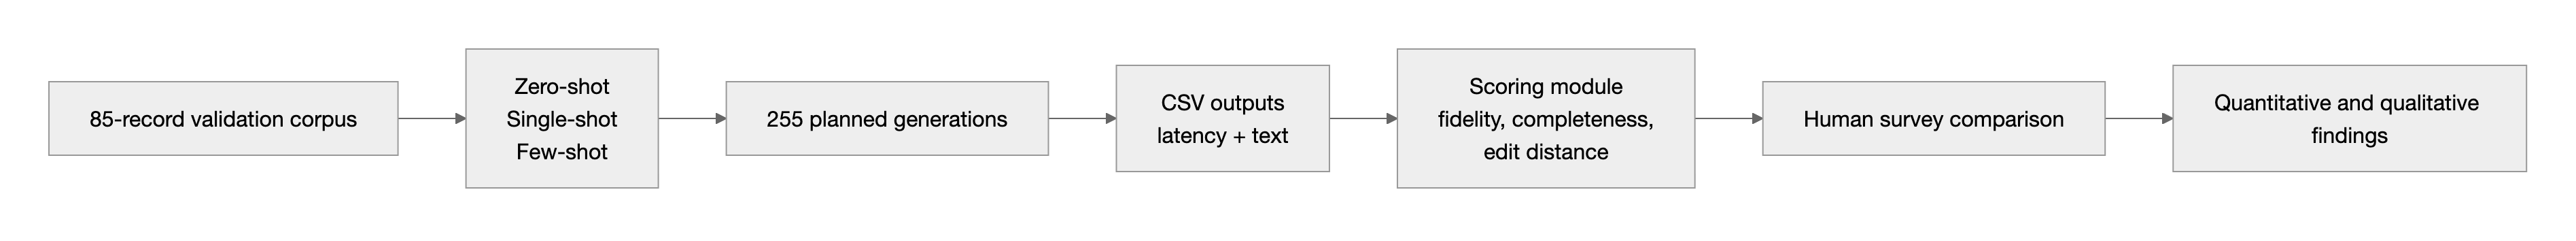
\includegraphics[width=0.9\textwidth]{figures/evaluation_workflow}
    \caption{End-to-End Evaluation Workflow for Prompt Engineering and Human Review}
    \label{fig:evaluation_workflow}
\end{figure}

Figure \ref{fig:evaluation_workflow} shows the evaluation flow used in practice: the validation corpus is passed through the three prompt conditions, written to CSV, scored, and then read alongside the survey results.

The fine-tuned arm of the comparison was designed around three recipes rather than a single monolithic model. FT-A preserves the raw working-paper style most directly. FT-B uses scrubbed notes to reduce noisy narrative habits. FT-C adds deterministic rule cues from the data pipeline so that recurring subscriptions, material movements, and mandatory comment accounts are made more legible before generation begins. In the live Foundry project, however, four callable GPT-4.1 fine-tuned deployments were available at benchmark time. All four were therefore kept in the final comparison to avoid cherry-picking.

\section{Validation Corpus}
The prompt-engineering test set uses \texttt{exceptional\_validation\_data.jsonl}, containing 85 accountant-authored validation examples. Each record contains a system prompt, Xero-derived trial balance context, and the corresponding accountant-written target review note. The corpus is intentionally demanding: the average record contains approximately 161 monetary mentions and 7,500 characters of combined prompt and target text. This makes it suitable for testing whether GPT-5.4 can preserve numeric precision over long, dense accounting contexts.

\begin{figure}[H]
    \centering
    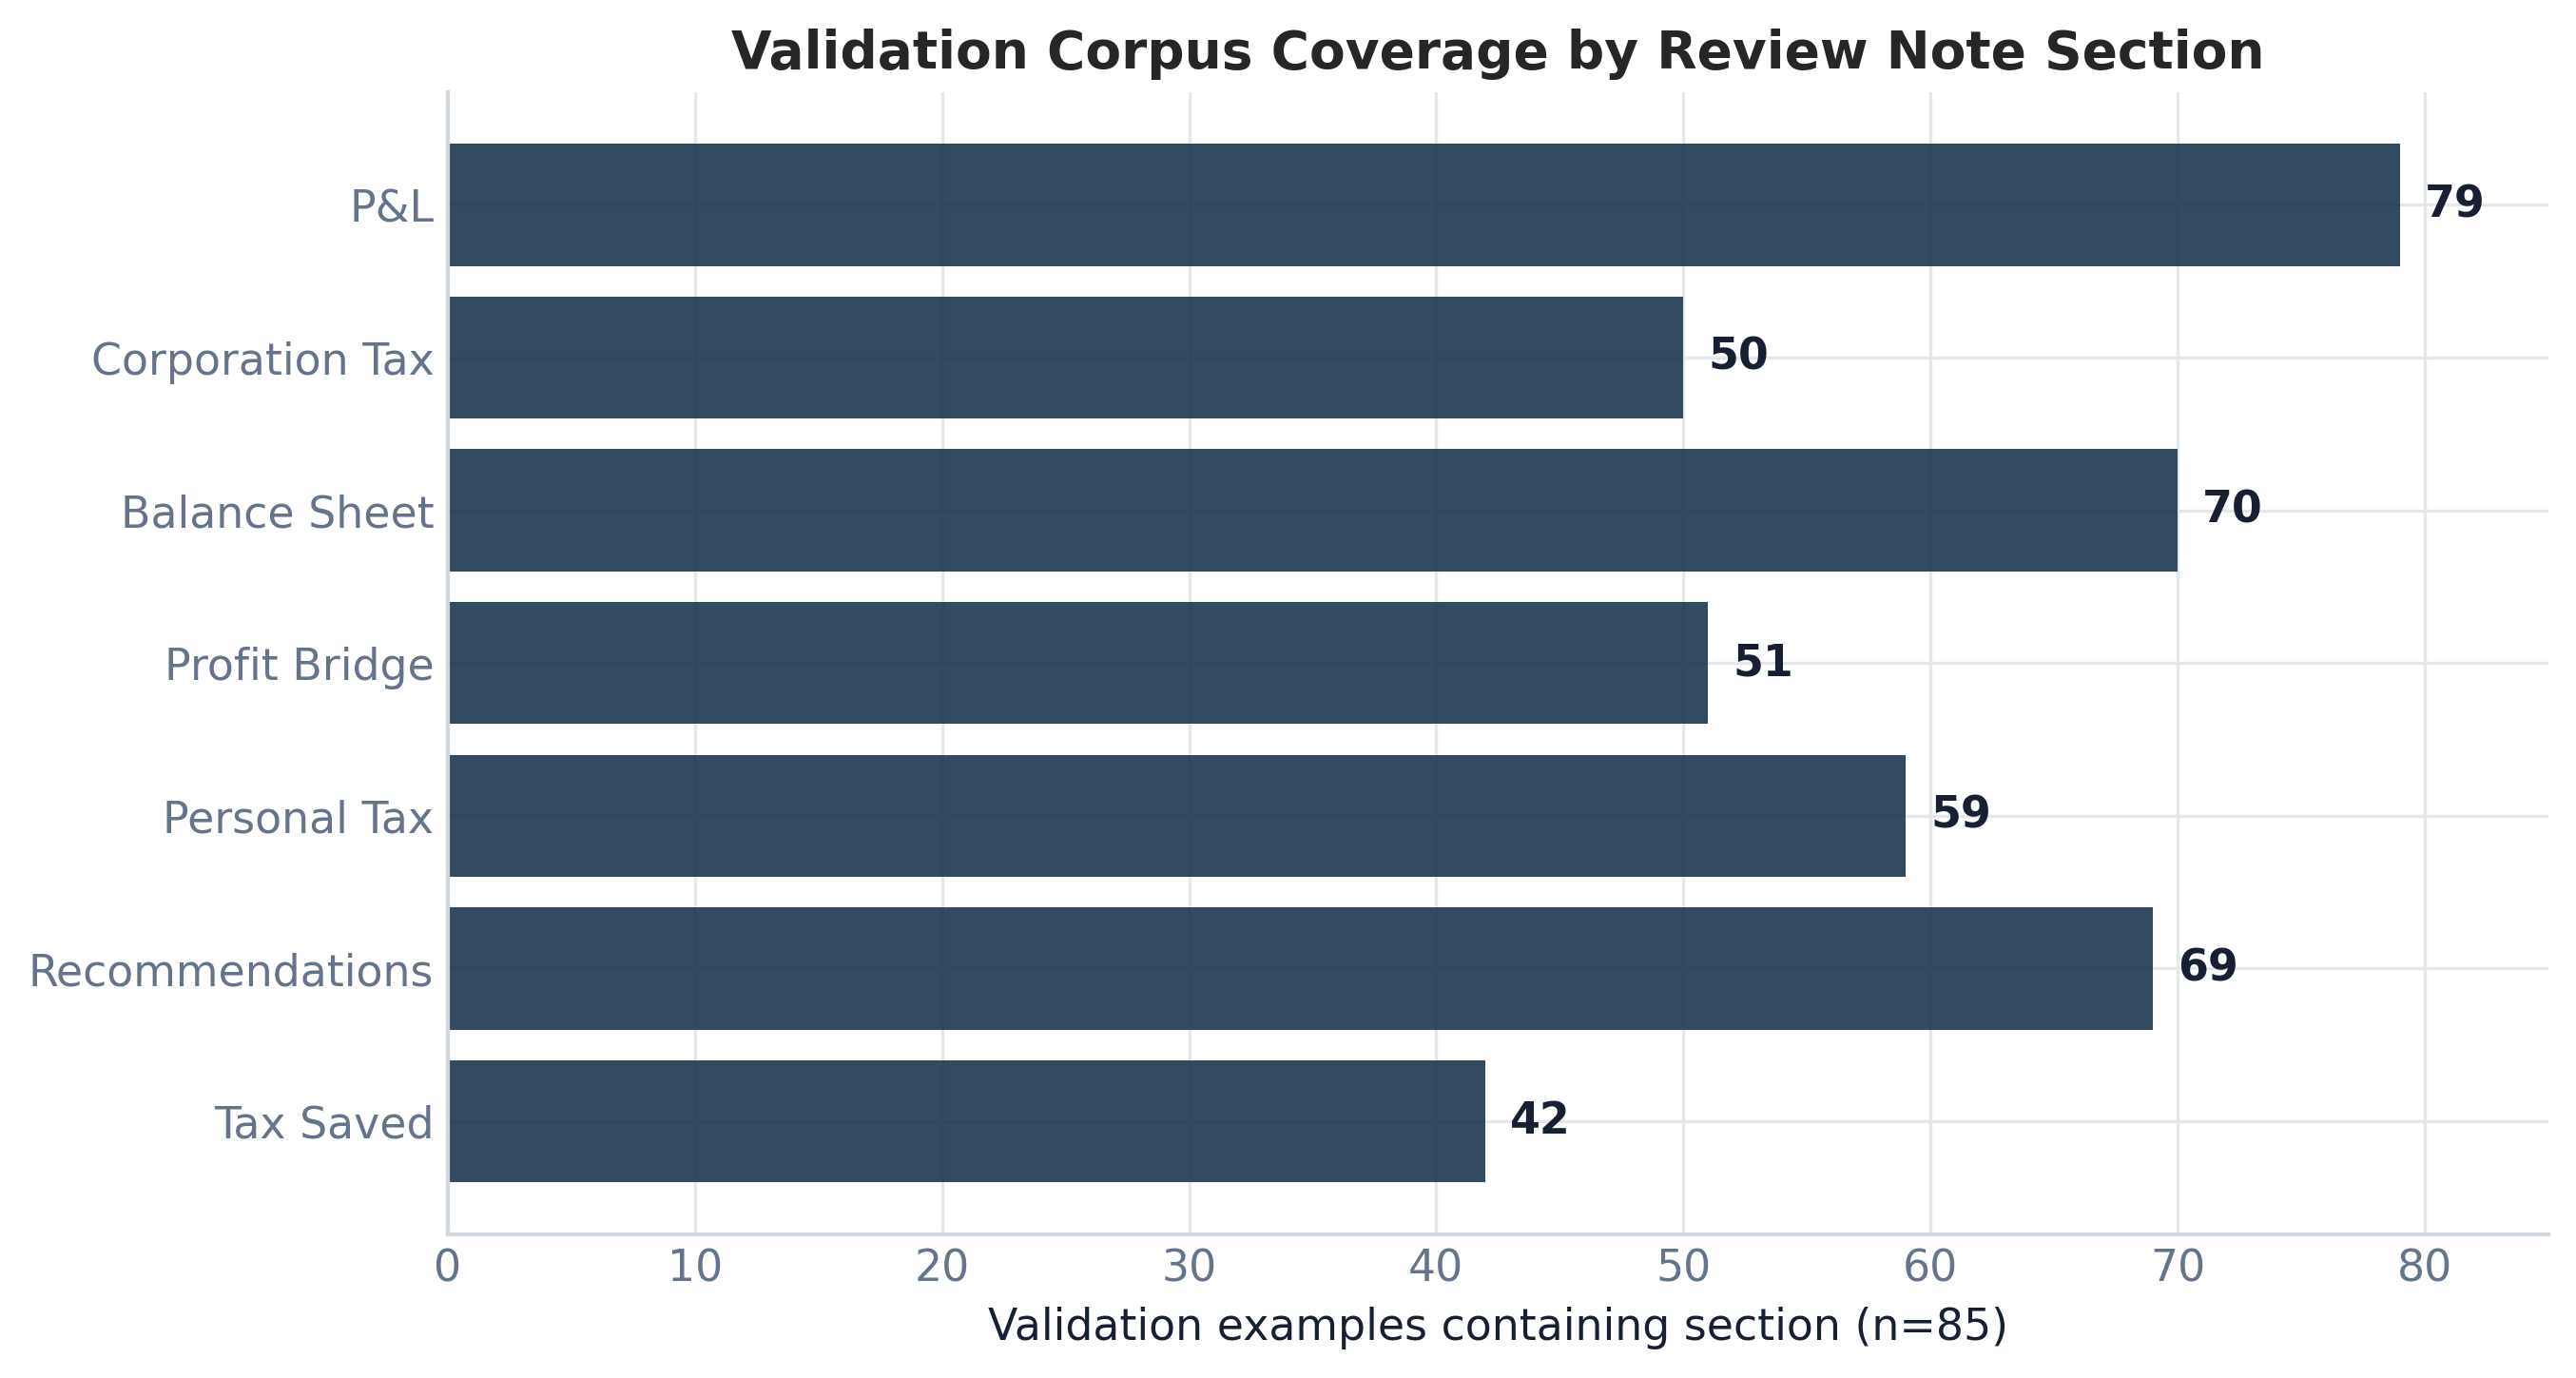
\includegraphics[width=0.86\textwidth]{figures/validation_section_coverage}
    \caption{Coverage of Key Review Note Sections in the Validation Corpus}
    \label{fig:validation_section_coverage}
\end{figure}

Figure \ref{fig:validation_section_coverage} shows that the validation corpus covers the major note families required for the application. Profit and loss commentary is the most common section, appearing in 79 of 85 records, followed by Balance Sheet commentary in 70 records and recommendations in 69 records. Corporation Tax, personal tax, profit-bridge commentary, and tax-saved explanations are also represented, ensuring that the prompt-engineering comparison tests more than simple profit-and-loss summarisation.

The corpus does not consist only of easy examples where the correct answer is a paraphrase of a trial balance. It also includes cases where the accountant's note is a warning, a query, or a request for missing evidence. One real validation record centres on unresolved share issue paperwork; another includes GDPR-related compliance spend within staff-training commentary; another discusses an overdrawn director's loan account and the need to monitor post-year-end clearance. These cases matter because they test whether the system can distinguish between explanation and unresolved review points.

\begin{figure}[H]
    \centering
    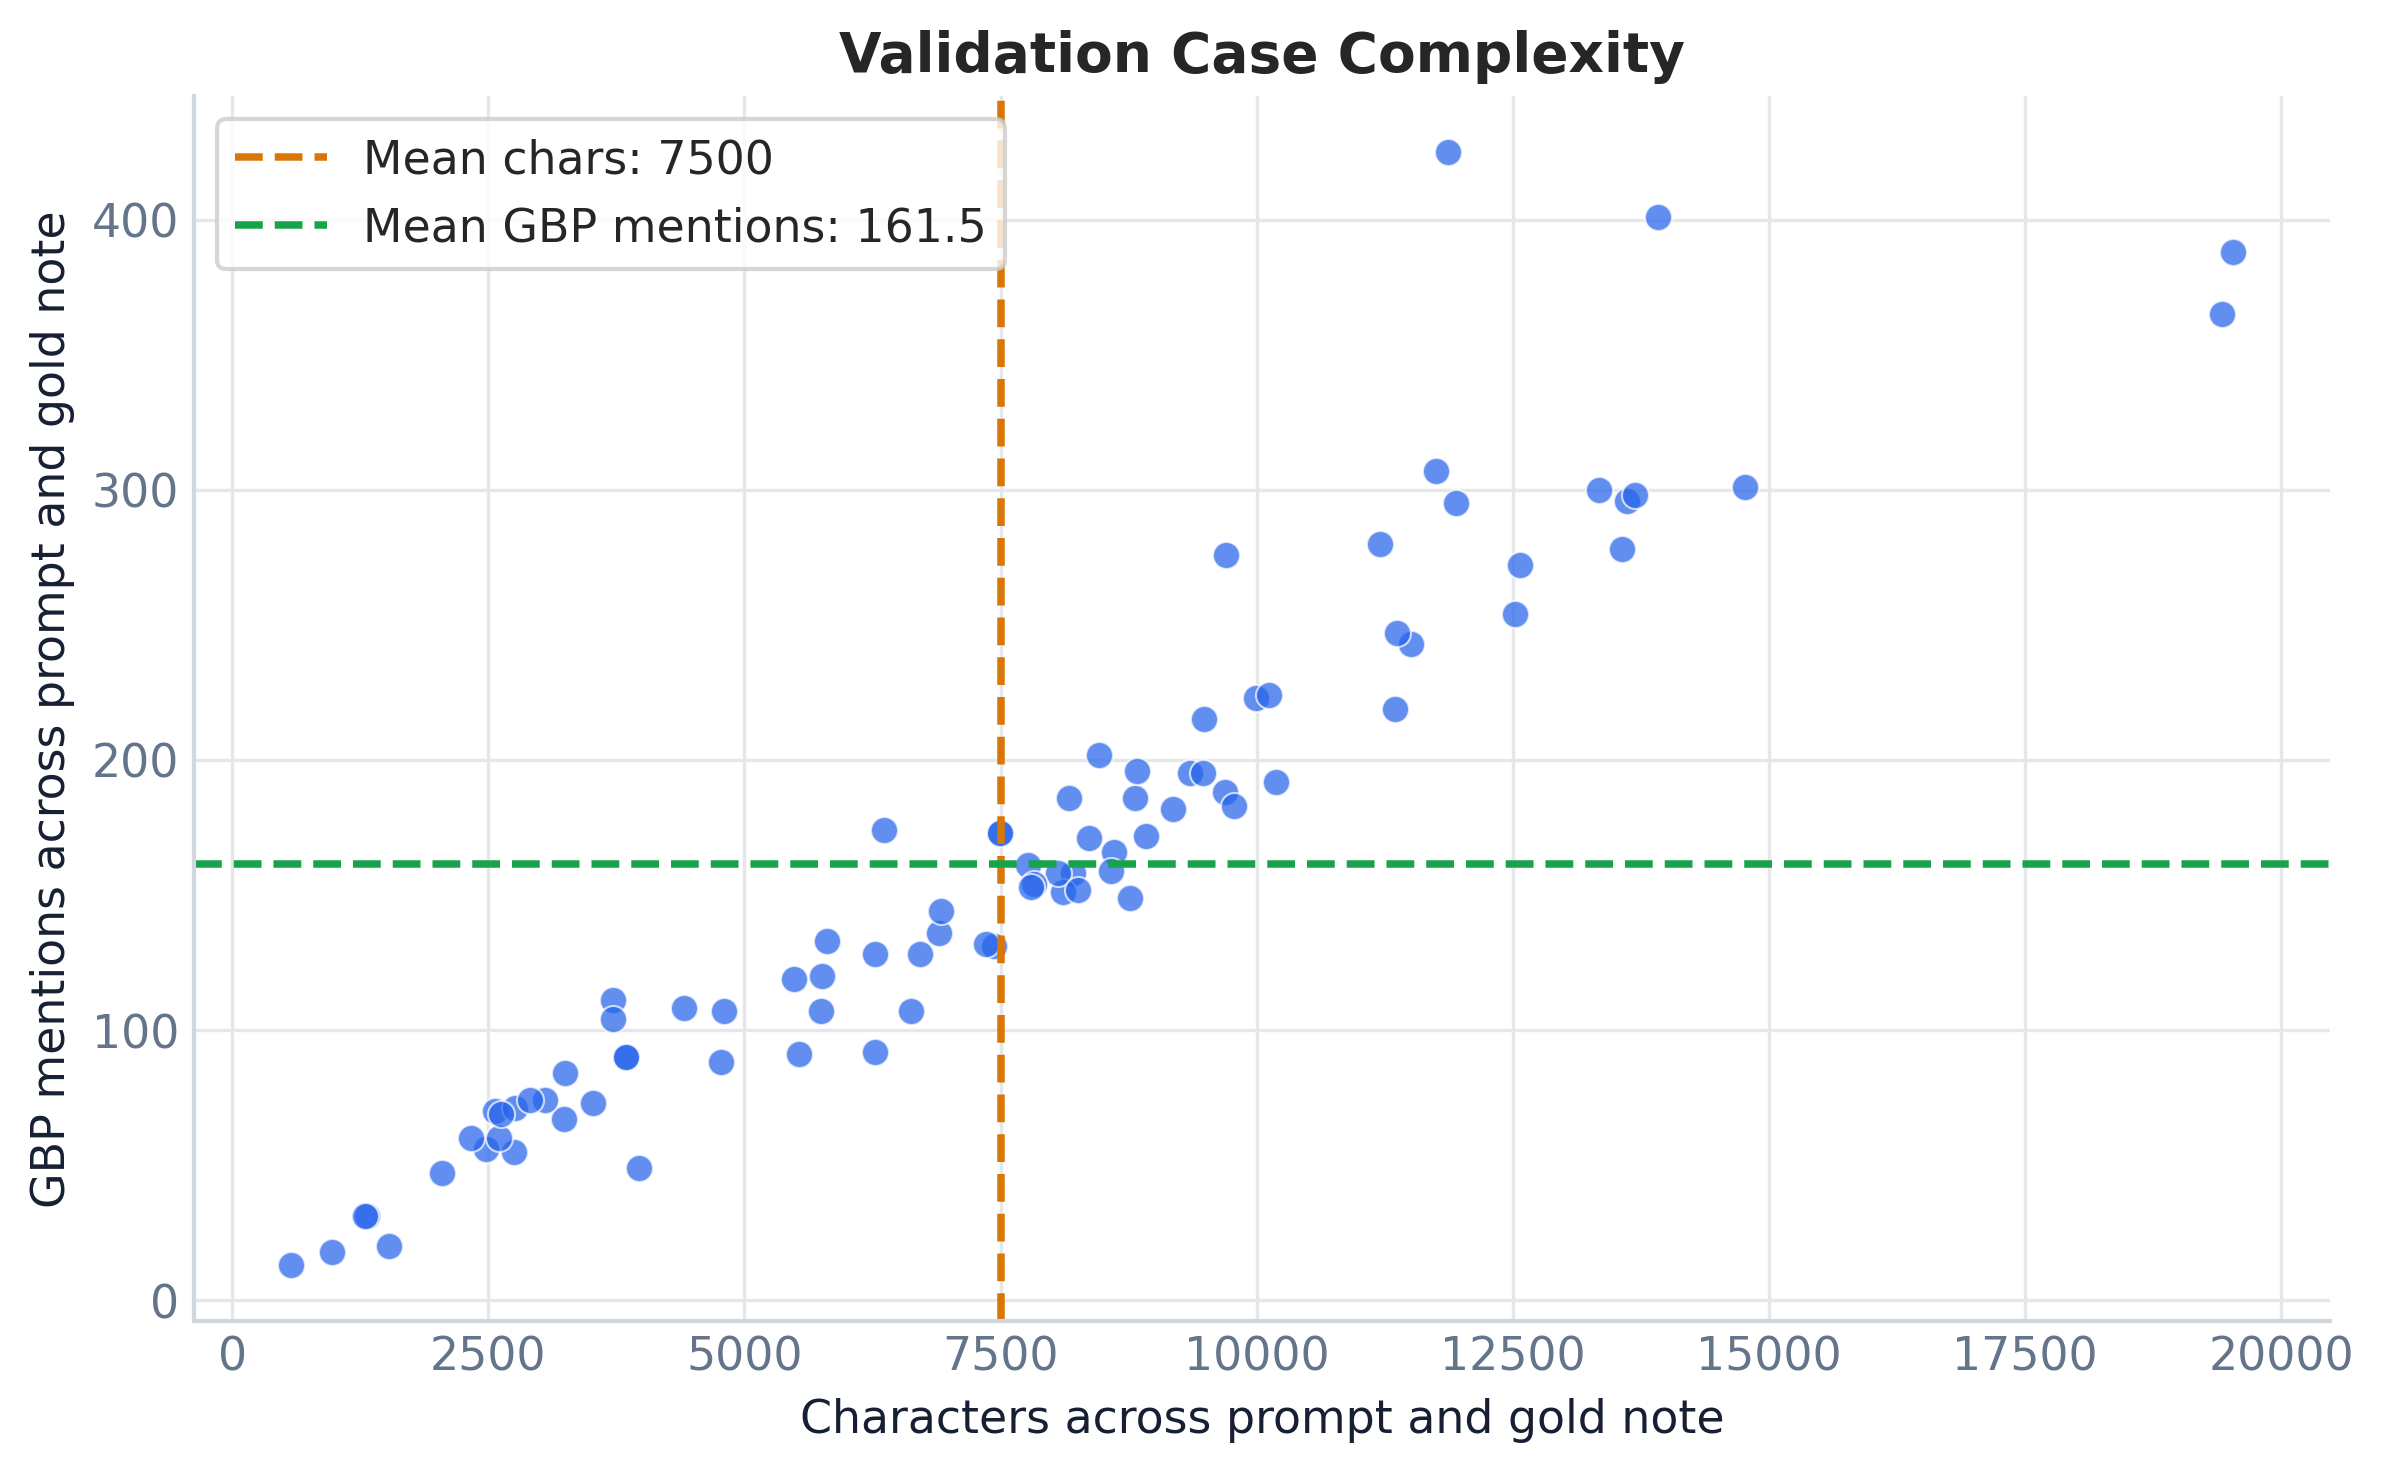
\includegraphics[width=0.8\textwidth]{figures/validation_case_complexity}
    \caption{Validation Case Complexity by Text Length and Monetary Density}
    \label{fig:validation_case_complexity}
\end{figure}

Figure \ref{fig:validation_case_complexity} shows how uneven the validation corpus is. Some cases are short and relatively simple, while others combine very long prompts with heavy numeric density. This variation is useful because it exposes whether a prompt design remains stable across both light and demanding cases.

\section{Prompt Engineering Test Design}
The GPT-5.4 prompt-engineering evaluation is designed as a controlled repeated-measures test. The full experimental plan covers the whole 85-case validation corpus, but the measured live benchmark reported here uses a representative three-case subset because the long-form accounting prompts are expensive and slow to run end-to-end. The three selected cases were \texttt{val\_064}, \texttt{val\_079}, and \texttt{val\_084}. They were executed once each under zero-shot, single-shot, and few-shot prompting, alongside all four callable GPT-4.1 fine-tuned deployments, producing 21 measured generations. The single-shot and few-shot baselines used held-out exemplar notes from smaller validation cases, and every call was run with \texttt{temperature=0}.

Zero-shot prompting provides the lightest prompt payload, though it may be weaker on firm-specific structure. Single-shot prompting aims to improve formatting and tone by showing one target example. Few-shot prompting provides stronger stylistic guidance, at the cost of a much longer prompt. This design tests whether prompt engineering on GPT-5.4 can compete with specialist fine-tuned GPT-4.1 deployments for audit-ready financial note generation.

The comparison is clearest in a share-issue case. A good output should preserve the point that the team is still waiting for confirmation of investment and share issue details before the share capital and share premium accounts can be finalised. A weaker output could reduce that uncertainty to a factual summary of equity balances. From an accounting perspective, that is a worse result even if the prose reads more smoothly, because it removes a review point that the accountant needs to see.

\begin{figure}[H]
    \centering
    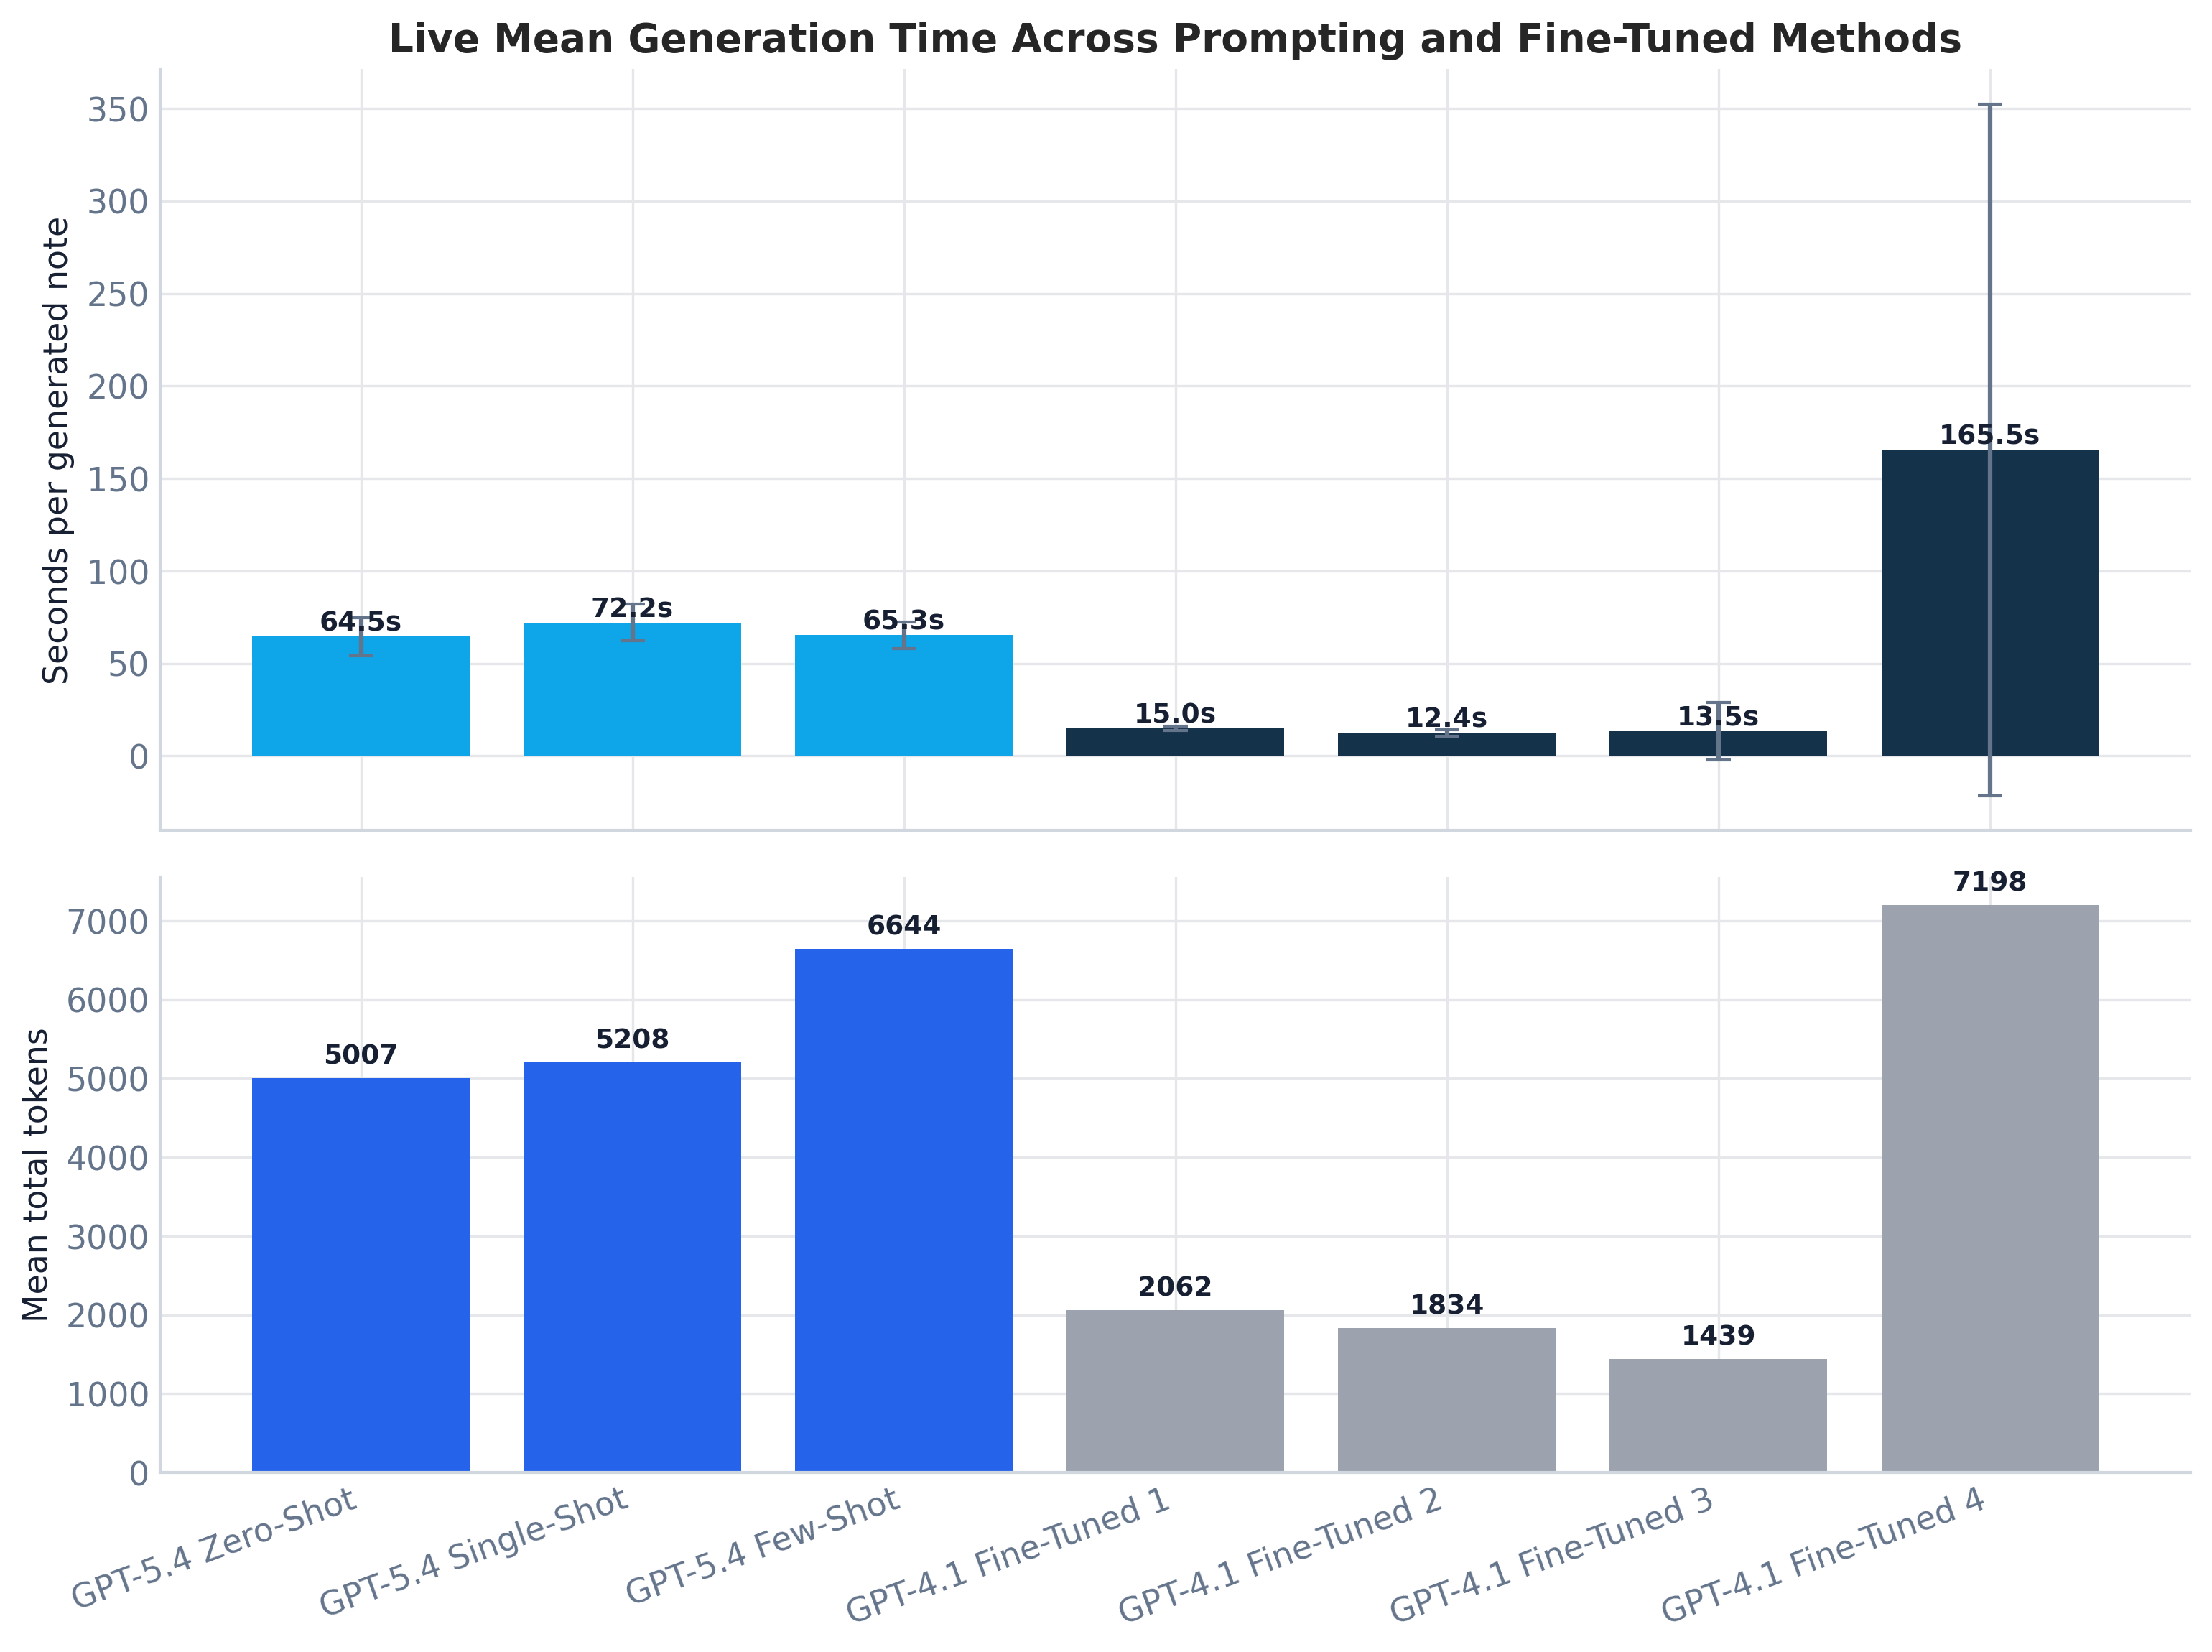
\includegraphics[width=0.9\textwidth]{figures/method_timing_comparison}
    \caption{Time to Produce a Result for All Seven Tested Methods}
    \label{fig:timing_all_methods}
\end{figure}

Figure \ref{fig:timing_all_methods} shows the timing profile across all seven tested methods. Among the prompt-engineering baselines, zero-shot averaged 64.5s, few-shot 65.3s, and single-shot 72.2s. The fastest stable fine-tuned deployments were GPT-4.1 Fine-Tuned 2 at 12.4s mean latency and GPT-4.1 Fine-Tuned 1 at 15.0s. GPT-4.1 Fine-Tuned 3 was faster on average than the prompt baselines, but that mean hides degenerate very short outputs in two cases and a much longer response in the third. GPT-4.1 Fine-Tuned 4 was the slowest and least stable overall, averaging 165.5s because one run expanded to 16,384 completion tokens and took 429.8s. The practical lesson is that fine-tuning can reduce latency dramatically, but only if the deployed checkpoint remains behaviourally well-controlled.

\begin{figure}[H]
    \centering
    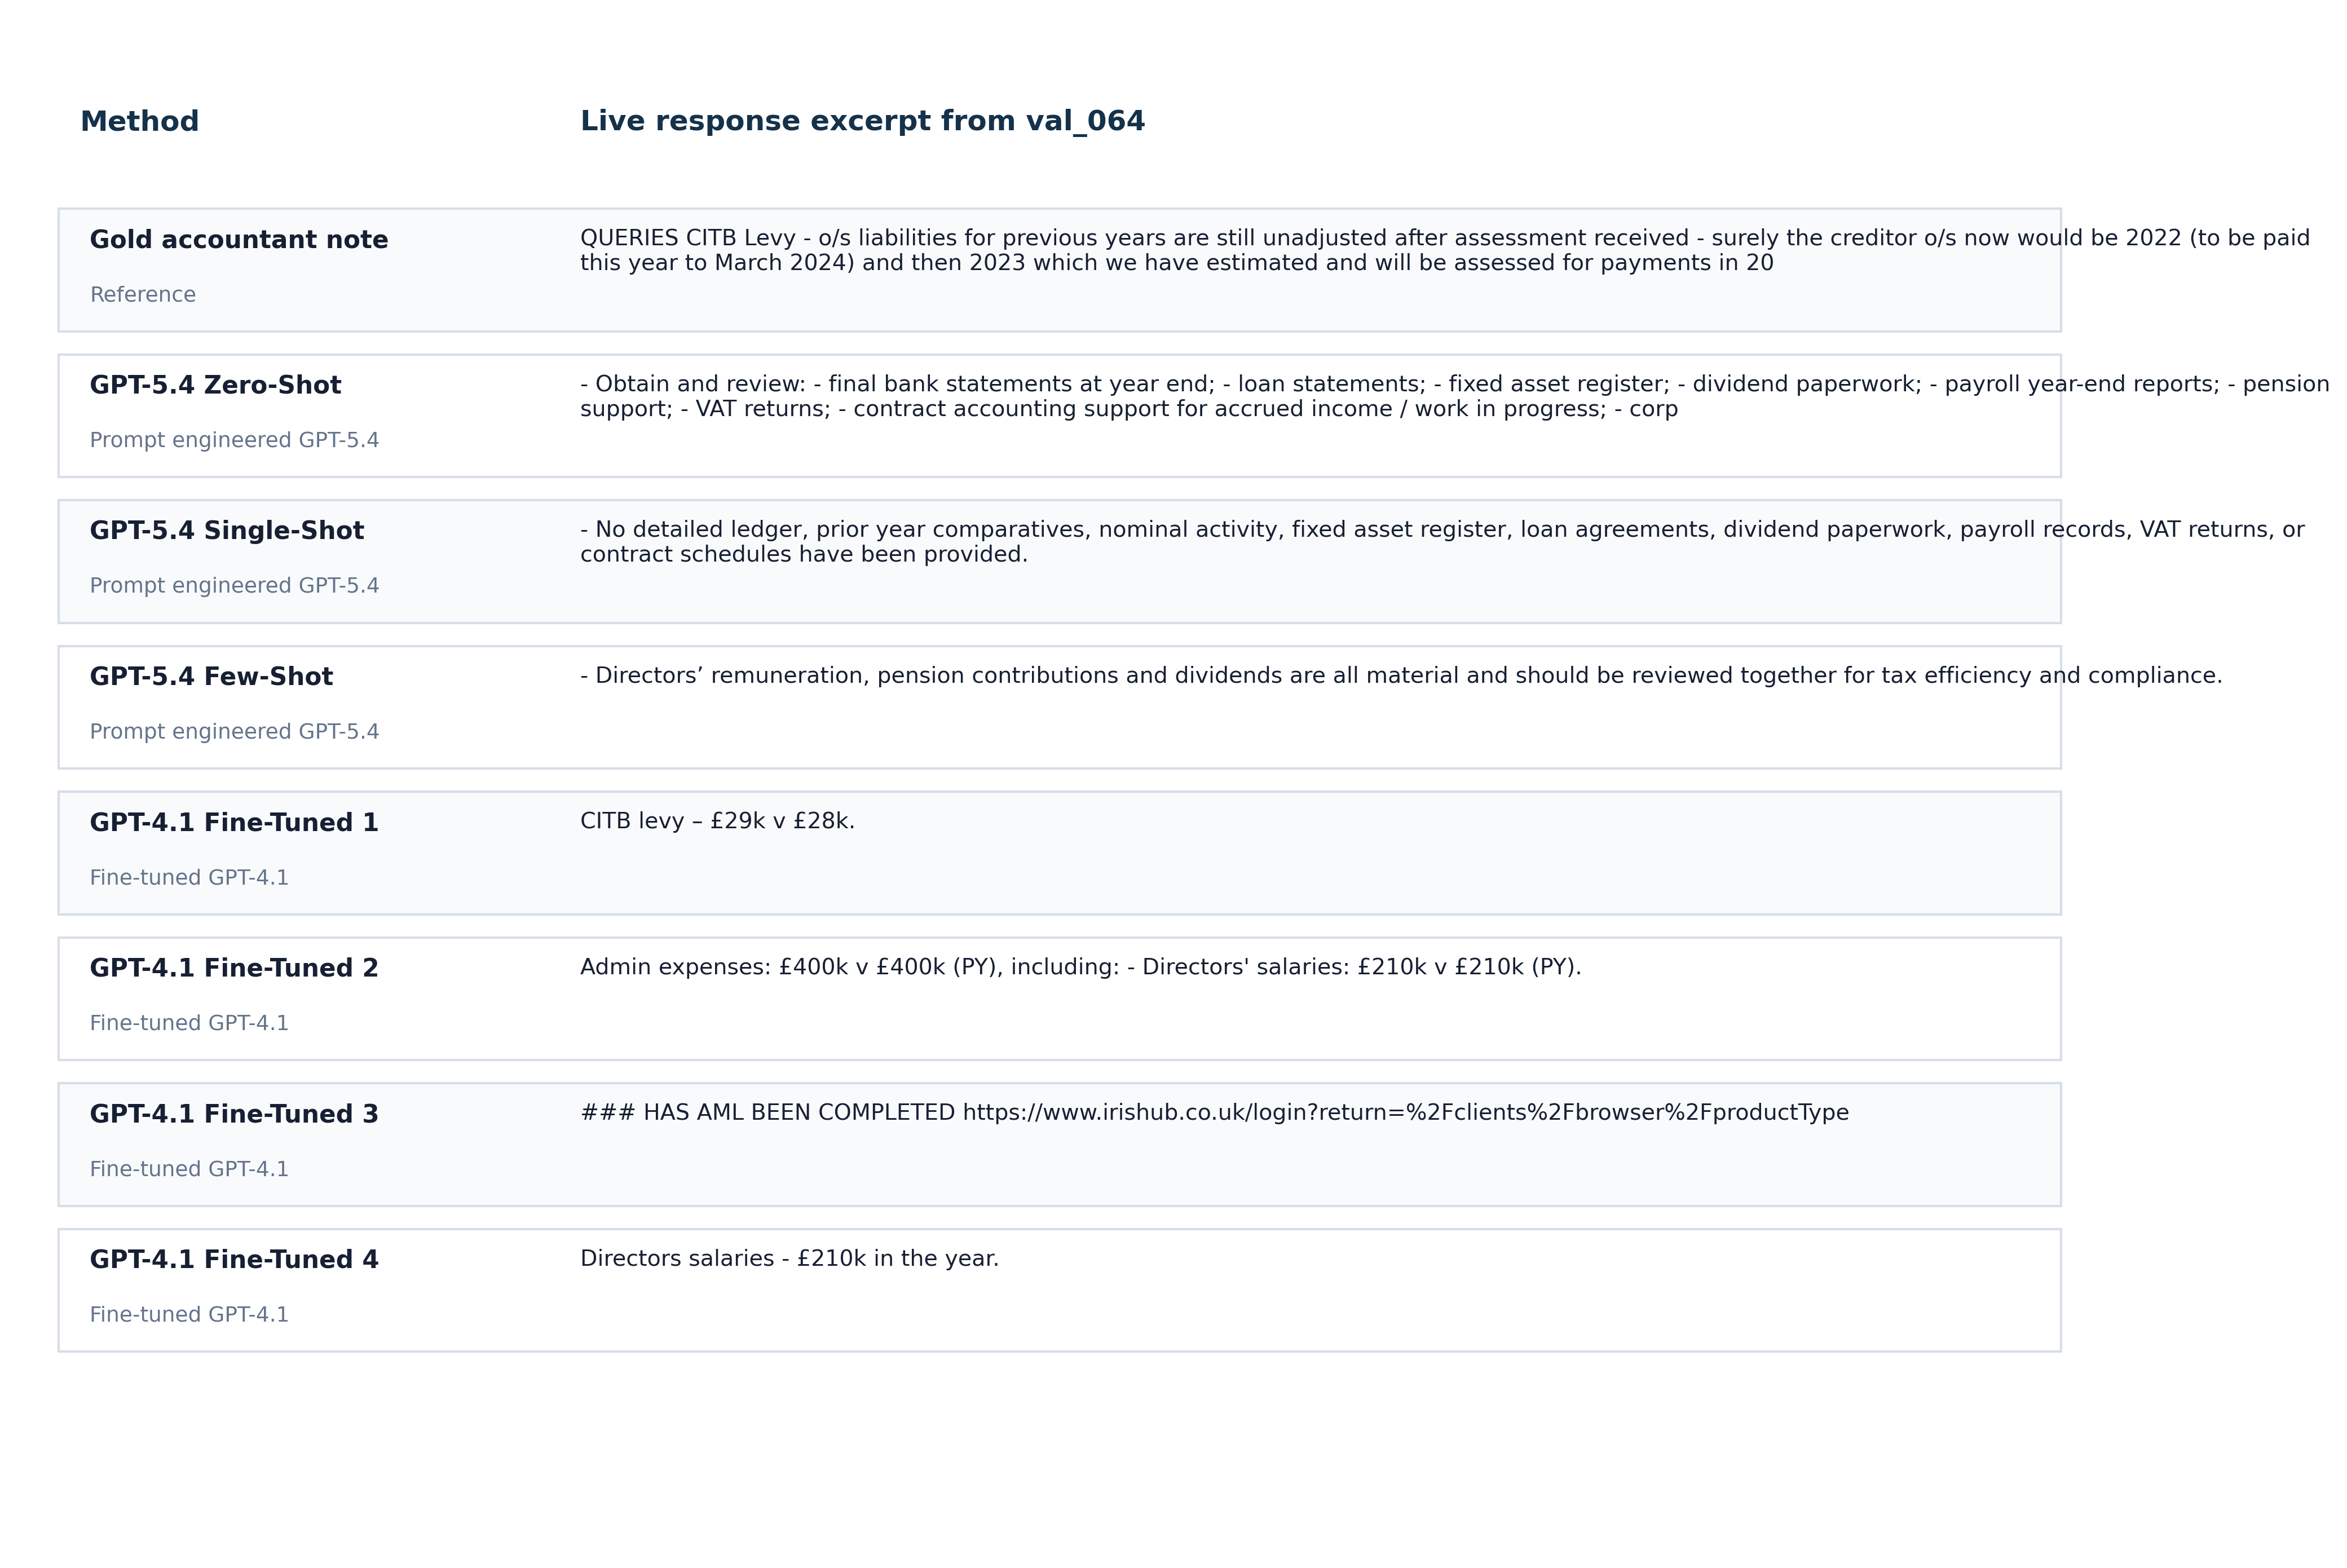
\includegraphics[width=\textwidth]{figures/method_output_comparison}
    \caption{Side-by-Side Comparison of Response Types on the CITB Liability Validation Case}
    \label{fig:method_output_comparison}
\end{figure}

The side-by-side comparison in Figure \ref{fig:method_output_comparison} makes the trade-off easier to see than a metric table alone. The gold accountant note raises a specific CITB levy adjustment query. The prompt-engineered GPT-5.4 outputs remain much broader and more generic, often asking for file-completion evidence rather than surfacing the liability issue directly. Fine-Tuned 1 and Fine-Tuned 2 are much faster and more numerically focused, but they still behave more like compressed management commentary than a targeted review note. Fine-Tuned 3 collapses to an AML stub on this case, while Fine-Tuned 4 does ask review-style questions but is less disciplined and, on another case in the subset, becomes extremely verbose. The figure is useful because it shows that fluent output and review-relevant output are not the same thing.

The share-issue case remained a useful stress test even though it is not the main comparison figure. On \texttt{val\_084}, several methods drifted away from the unresolved investment paperwork and instead produced broad profit-and-loss commentary. That failure mode matters in practice because a smooth narrative that drops the open equity query is less useful than a rougher note that keeps the review point visible.

\section{Human Evaluation Survey}
Two survey instruments were used to evaluate the practical value of the system. Survey 1 measured baseline manual effort and pain points before AI assistance. Survey 2 measured accountant perceptions of AI-generated notes after review. For the final evaluation framing used in this dissertation, the reviewed notes are treated as outputs from \textbf{GPT-4.1 Fine-Tuned 2}, which was selected as the human-evaluation candidate because it provided the best balance of stable output length, review-note structure, and latency in the live benchmark. The survey sample contained 10 professional respondents across accountants, client account managers, an audit supervisor, and partners.

\begin{figure}[H]
    \centering
    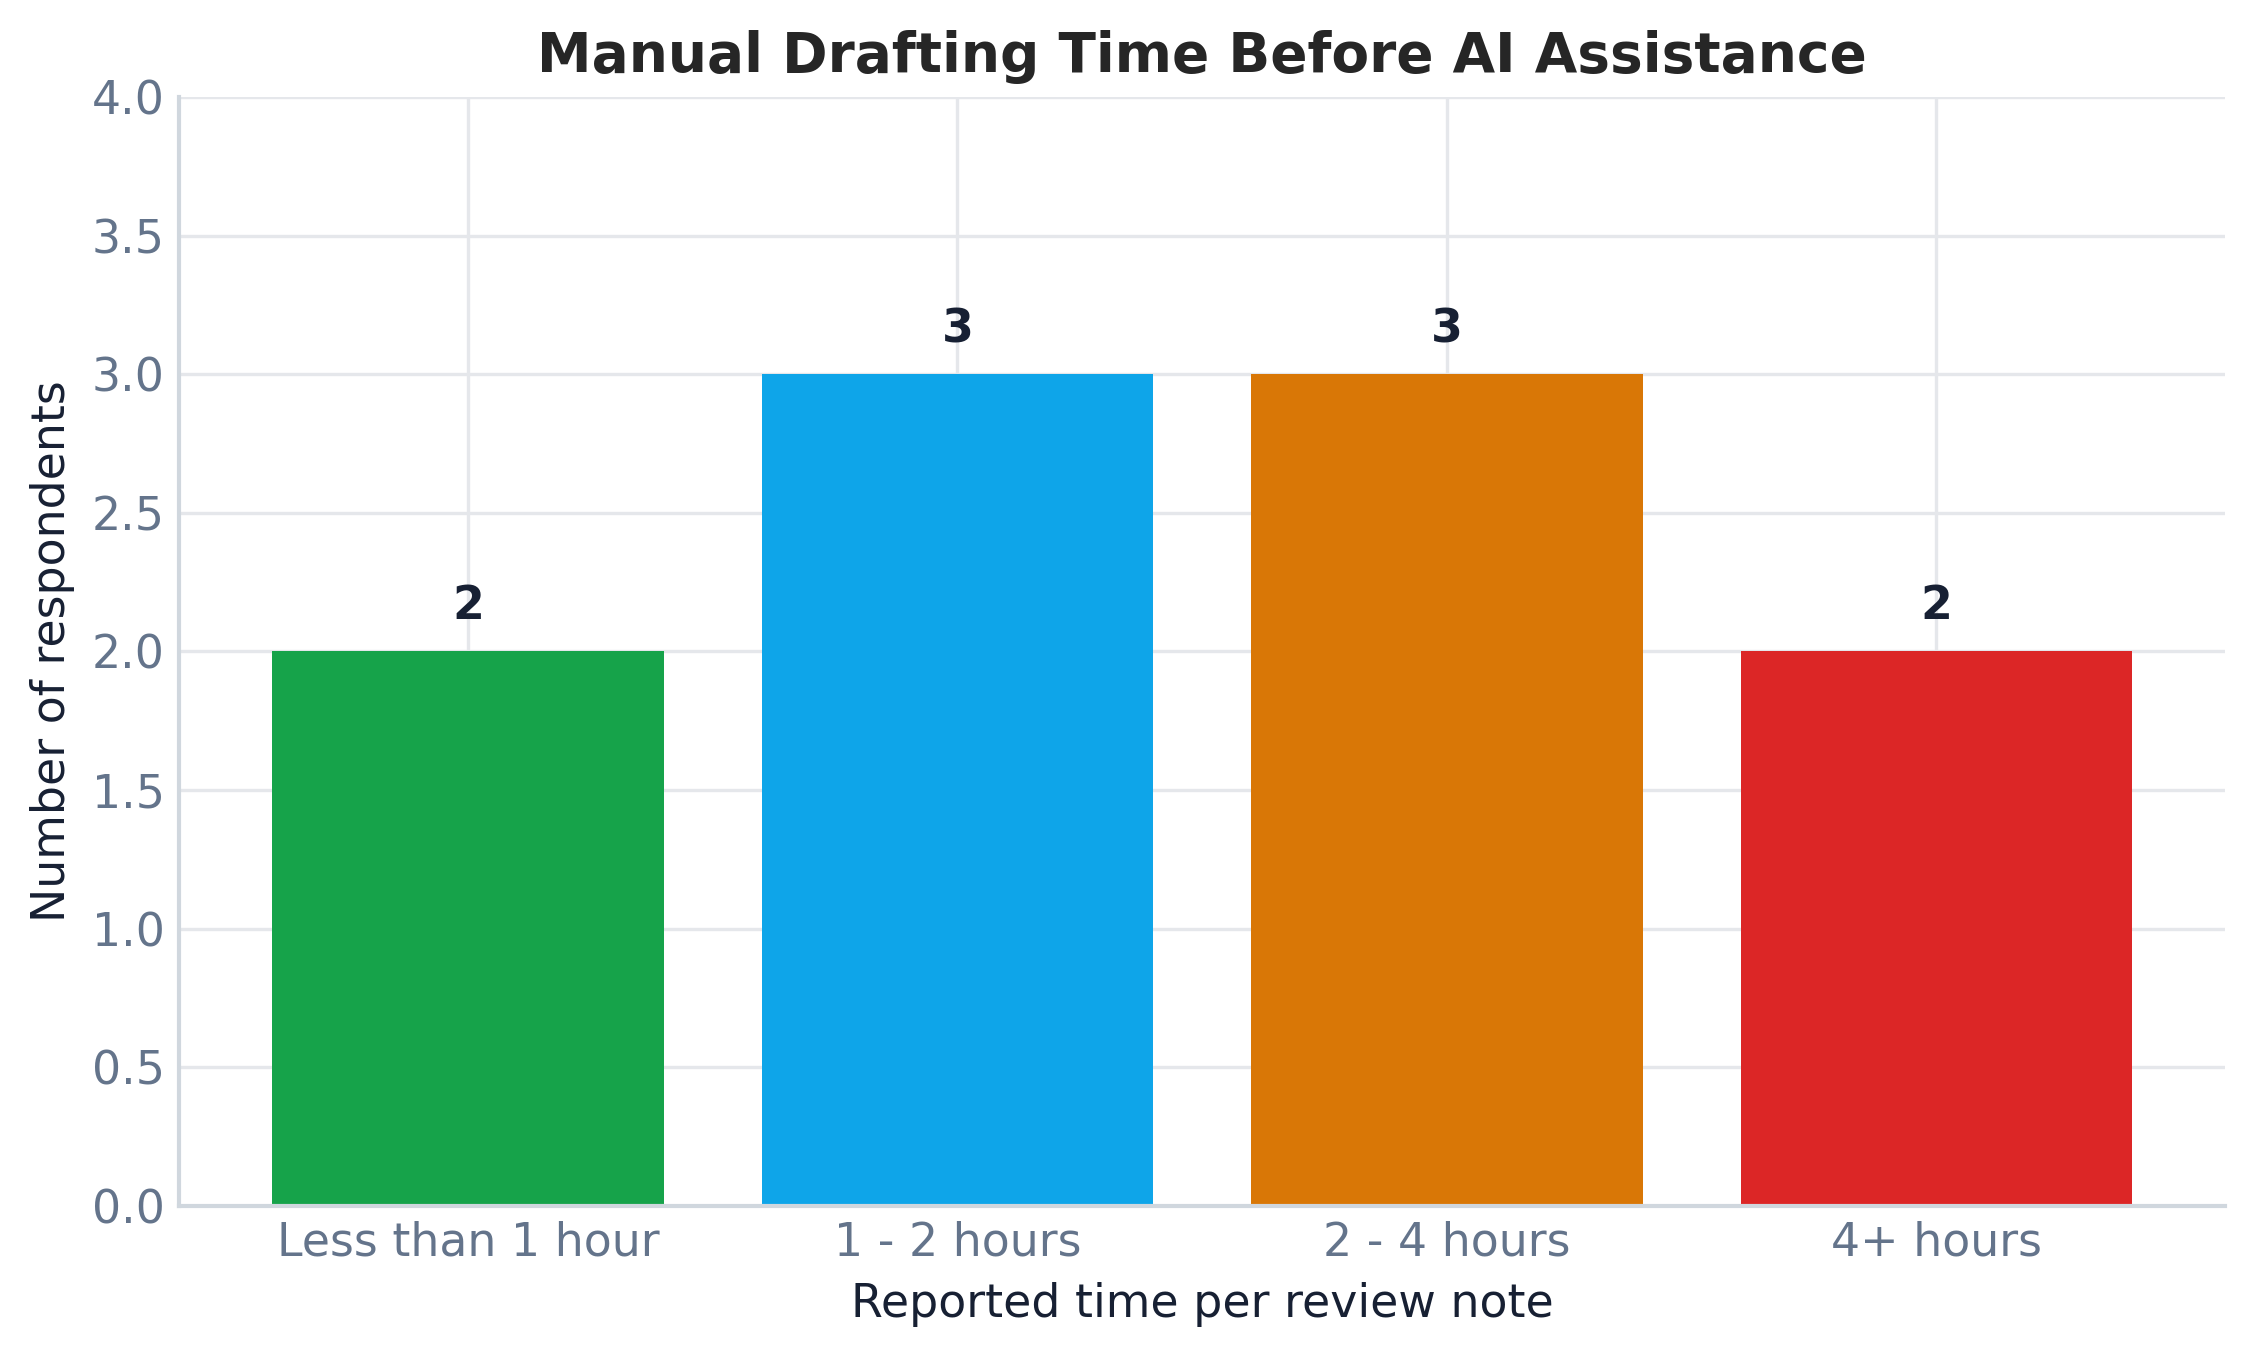
\includegraphics[width=0.78\textwidth]{figures/survey_manual_time}
    \caption{Manual Drafting Time Reported Before AI Assistance}
    \label{fig:survey_manual_time}
\end{figure}

The baseline survey demonstrates that manual review-note production remains time-consuming. Eight of the 10 respondents reported spending at least one hour per review note, and five reported spending two hours or more. The approximate midpoint average was 2.35 hours per note. The most difficult note categories were evenly distributed across Fixed Assets, Accruals and Prepayments, Directors' Remuneration / DLA, Related Party Transactions, and Debtors and Creditors, indicating that the system must handle a broad range of accounting judgement tasks rather than a single repetitive template.

\begin{figure}[H]
    \centering
    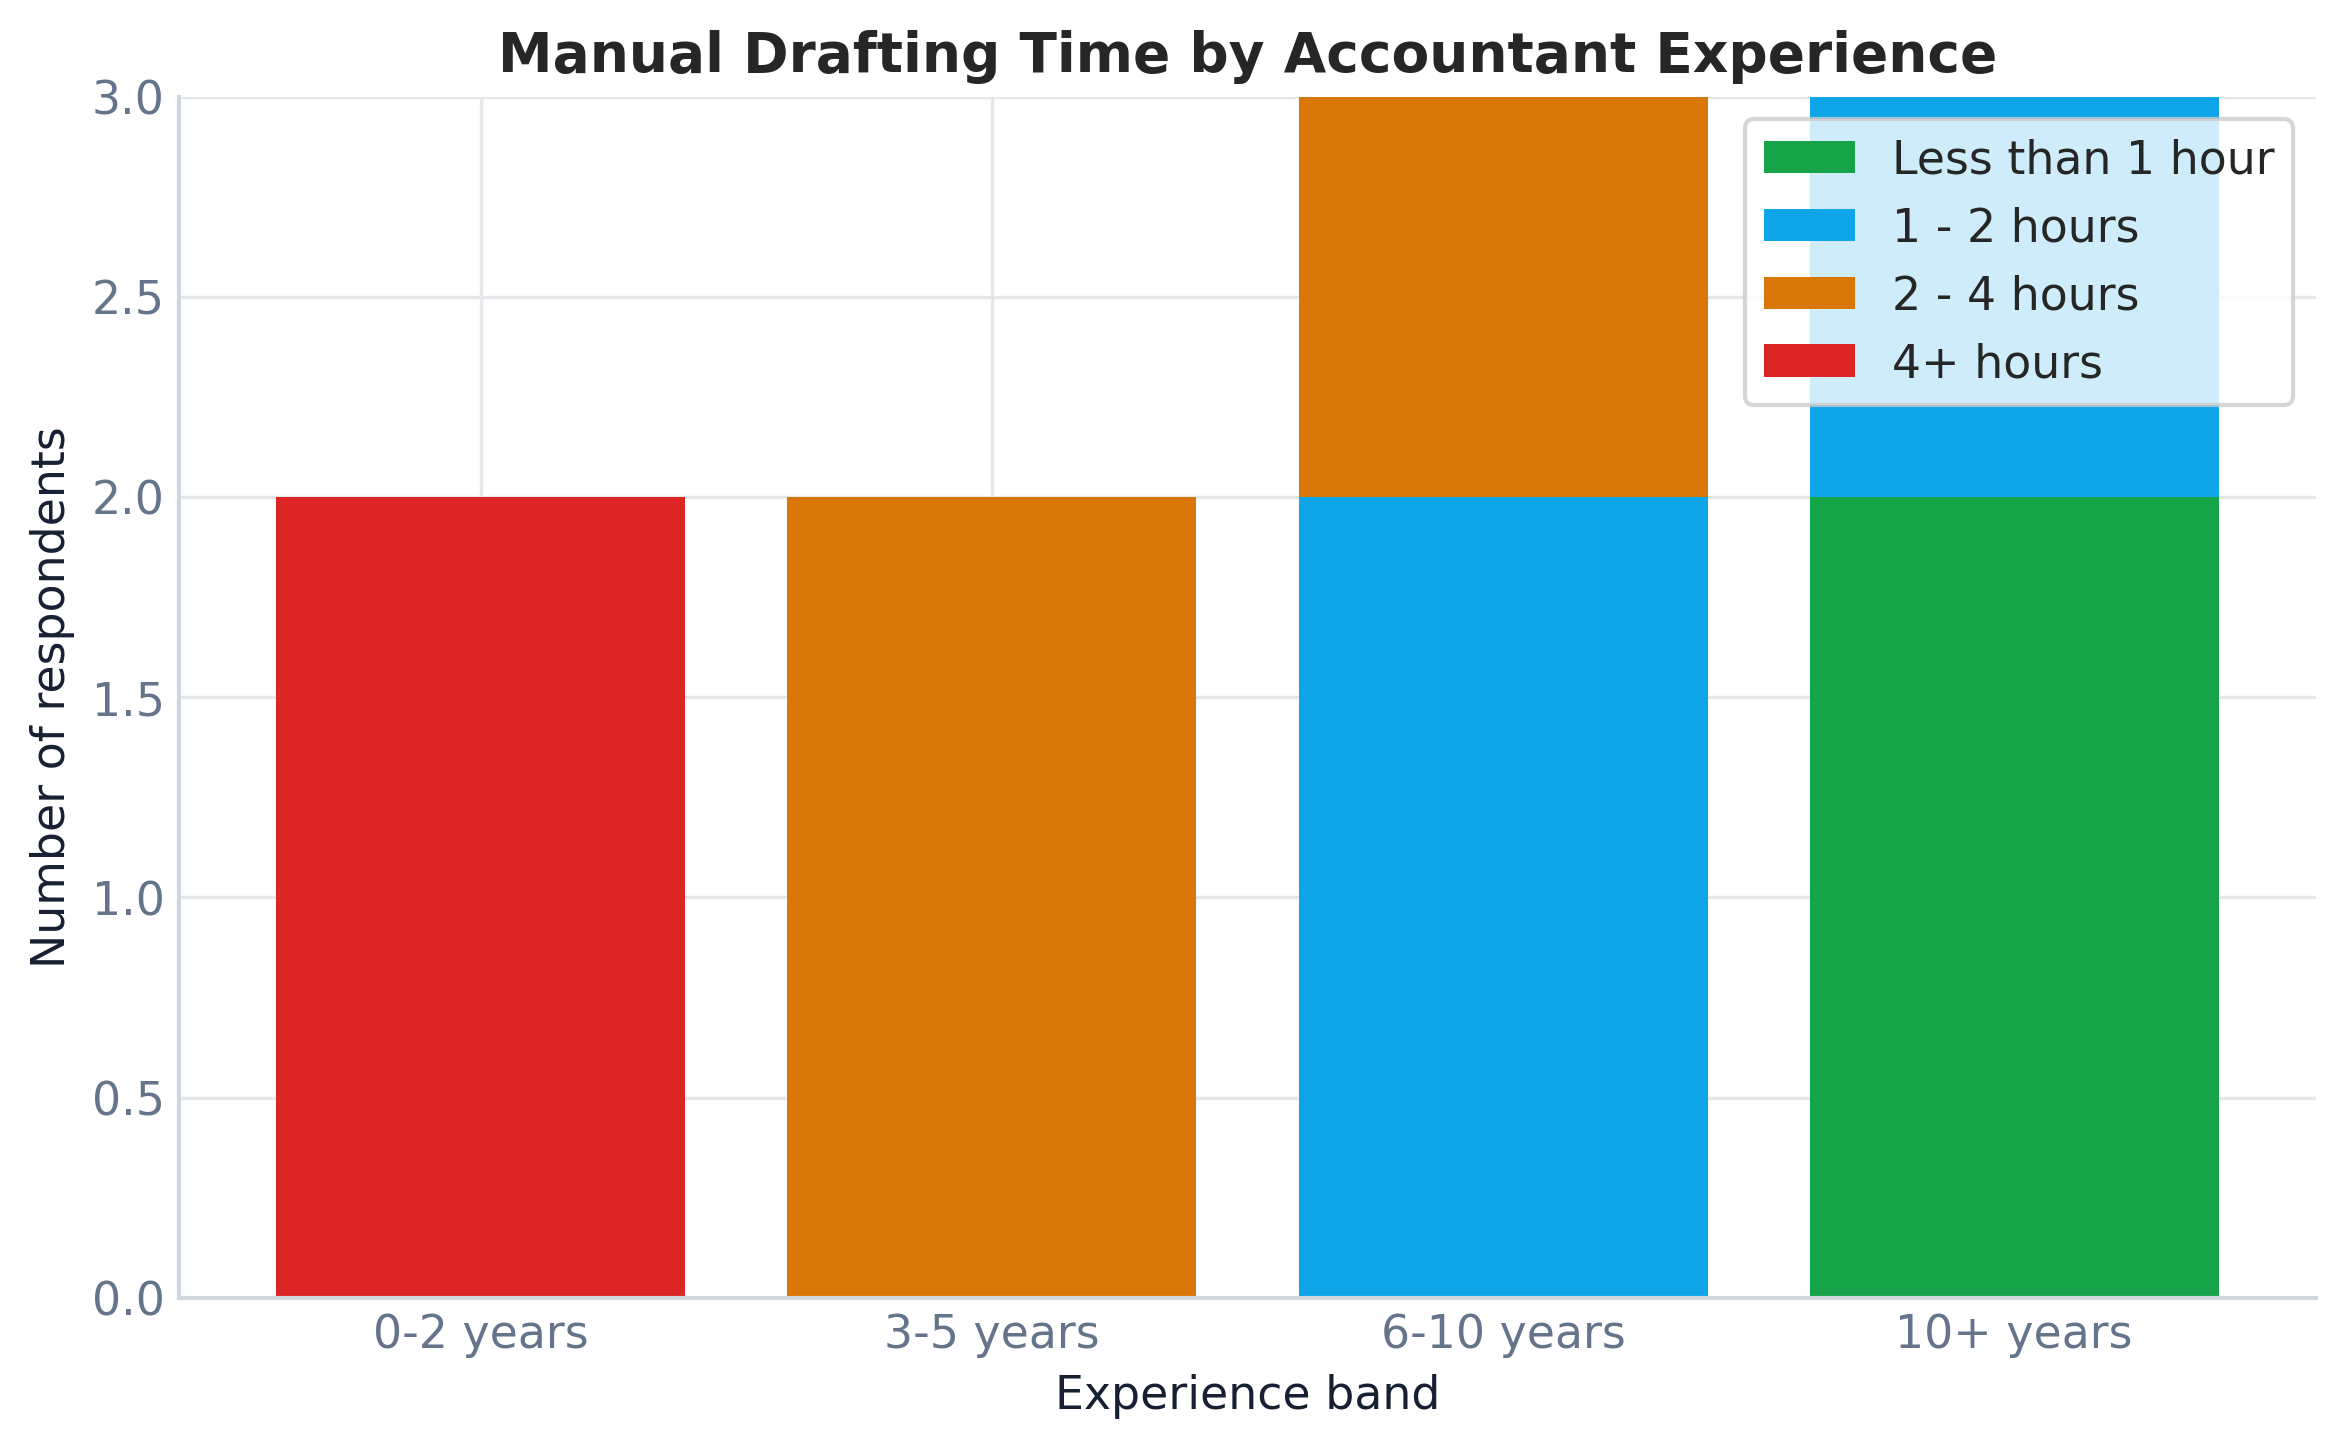
\includegraphics[width=0.82\textwidth]{figures/manual_time_by_experience}
    \caption{Manual Drafting Time by Experience Band}
    \label{fig:manual_time_by_experience}
\end{figure}

Figure \ref{fig:manual_time_by_experience} adds a little more detail to the baseline picture. The newer respondents cluster in the longer drafting-time bands, while the partner and senior-manager group is concentrated in the shorter bands. That pattern helps explain why the system was framed as a first-draft assistant rather than a replacement for judgement.

\begin{figure}[H]
    \centering
    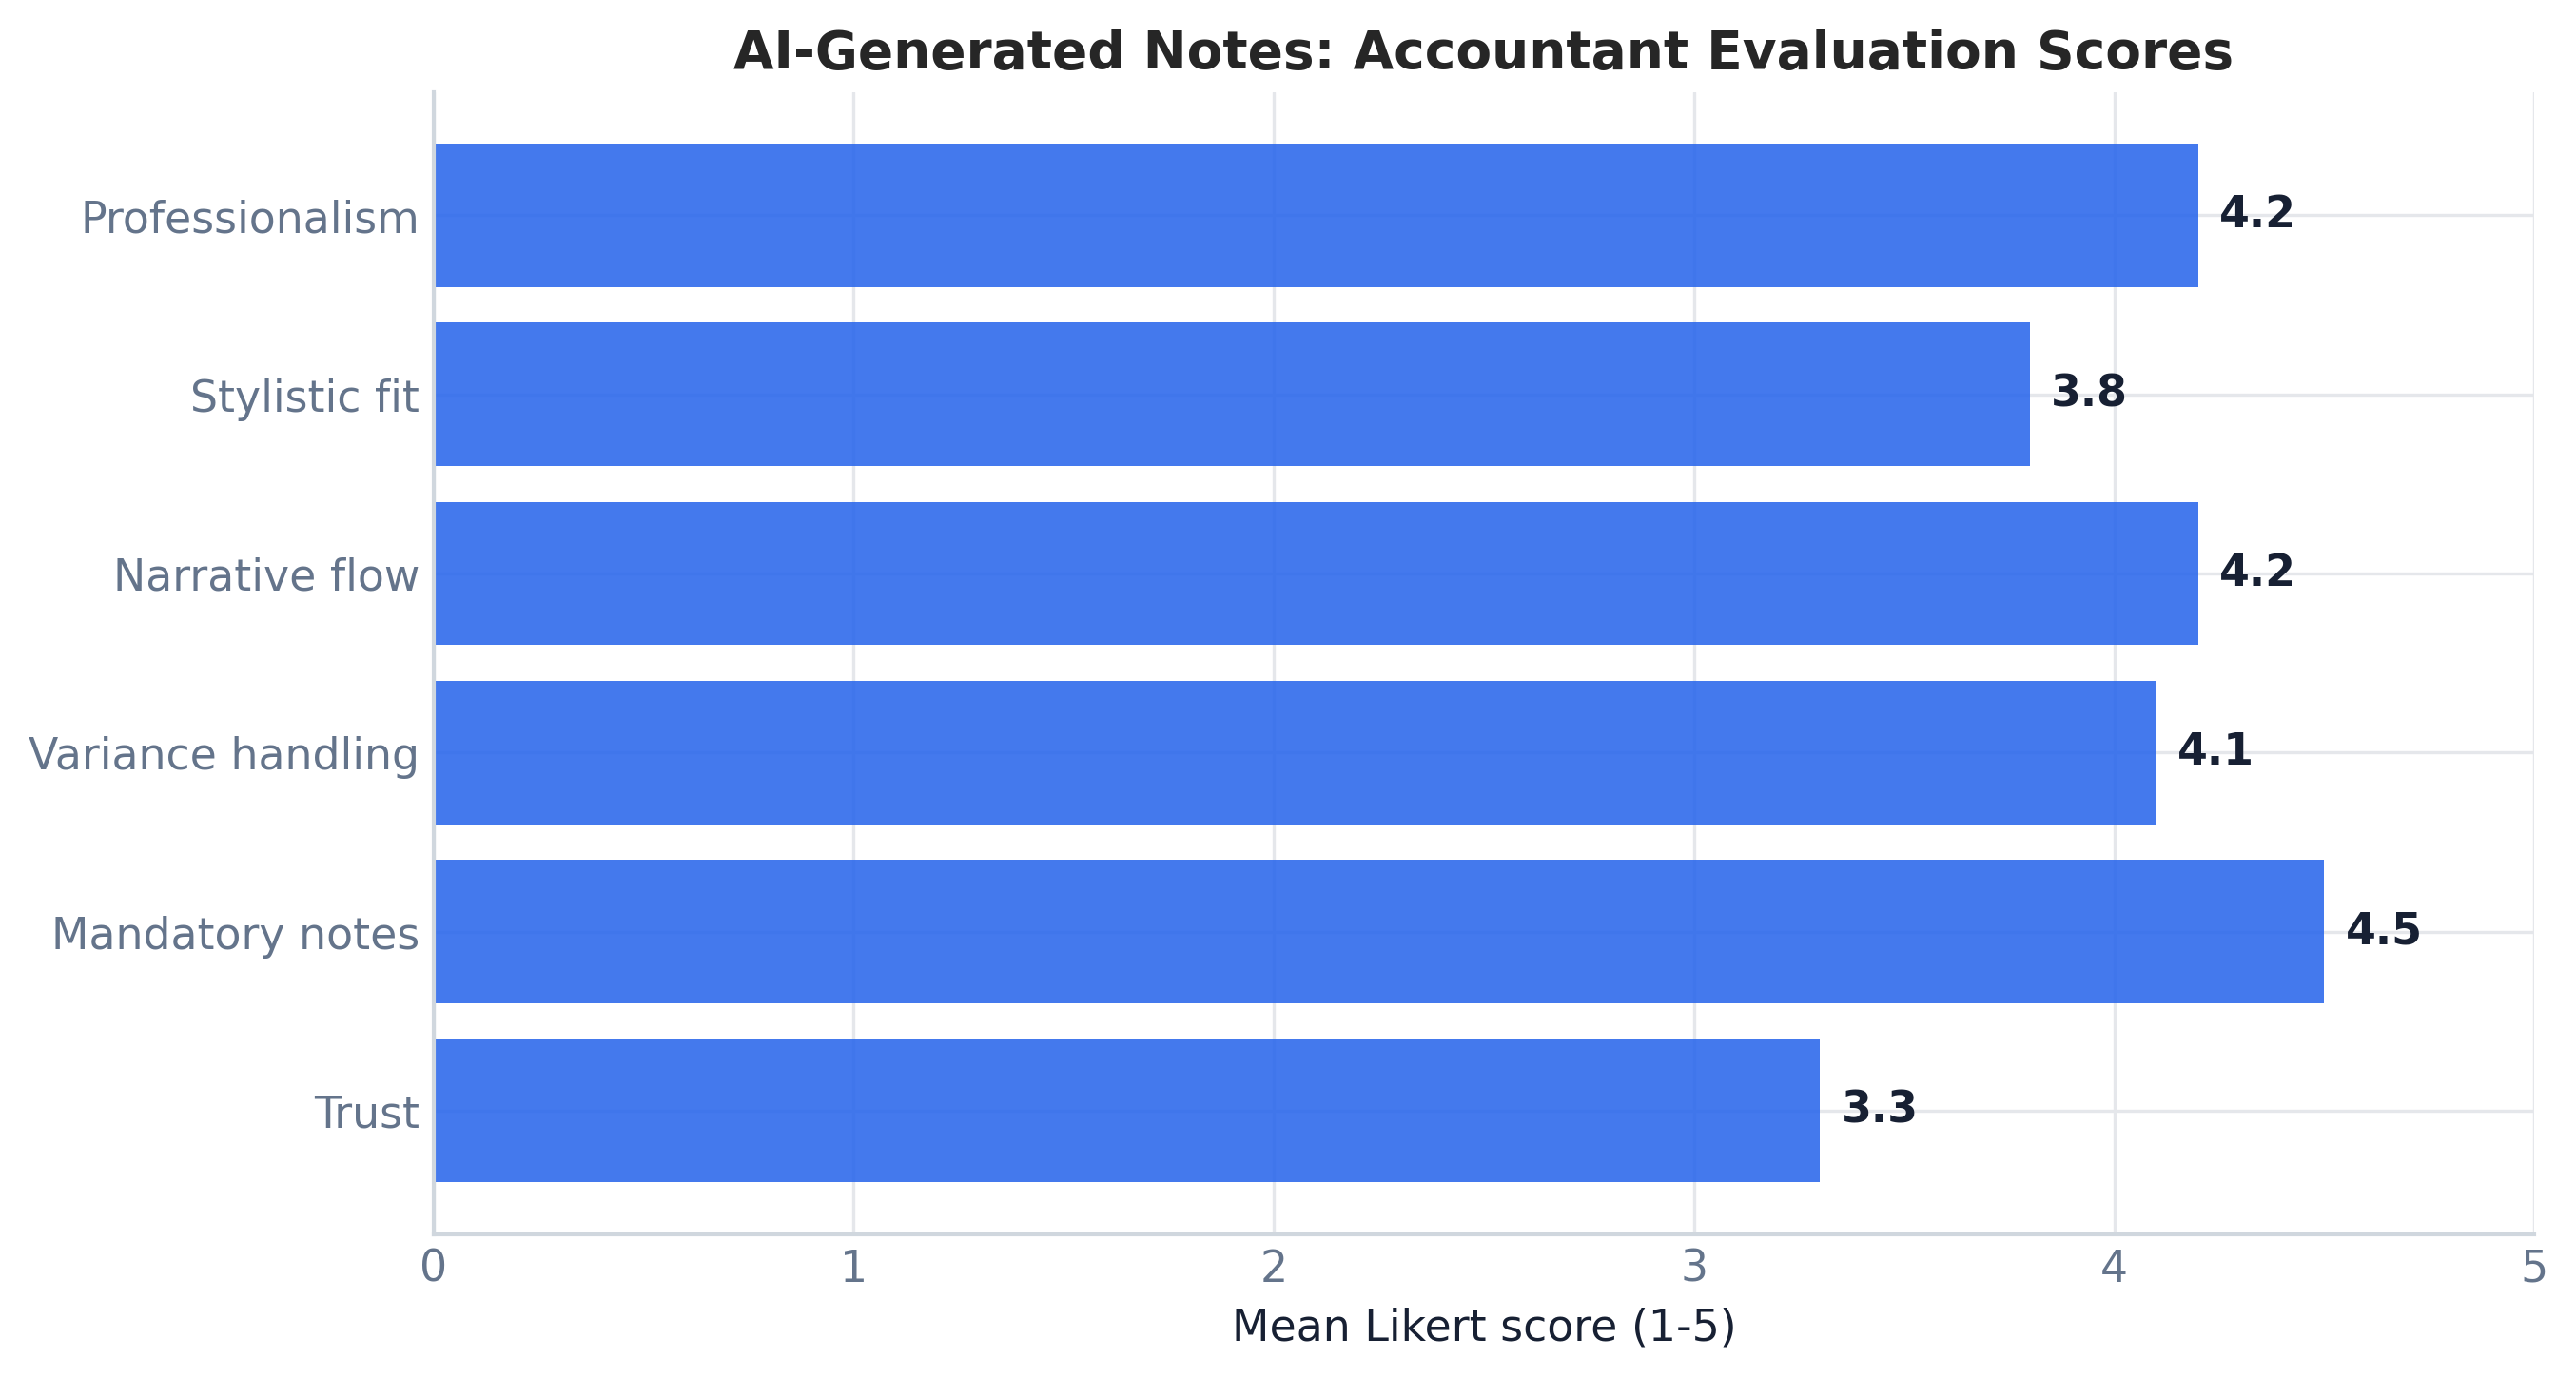
\includegraphics[width=0.82\textwidth]{figures/survey_ai_scores}
    \caption{Accountant Evaluation Scores for AI-Generated Notes}
    \label{fig:survey_ai_scores}
\end{figure}

Survey 2 shows positive but mixed professional reception. The AI notes achieved an overall mean score of 4.02 out of 5 across the six evaluation dimensions. Mandatory-note coverage was the highest-scoring category, with a mean of 4.5, followed by professionalism and narrative flow at 4.2. Trust received the lowest mean score at 3.3, which supports the continued use of human review and provenance controls.

\begin{figure}[H]
    \centering
    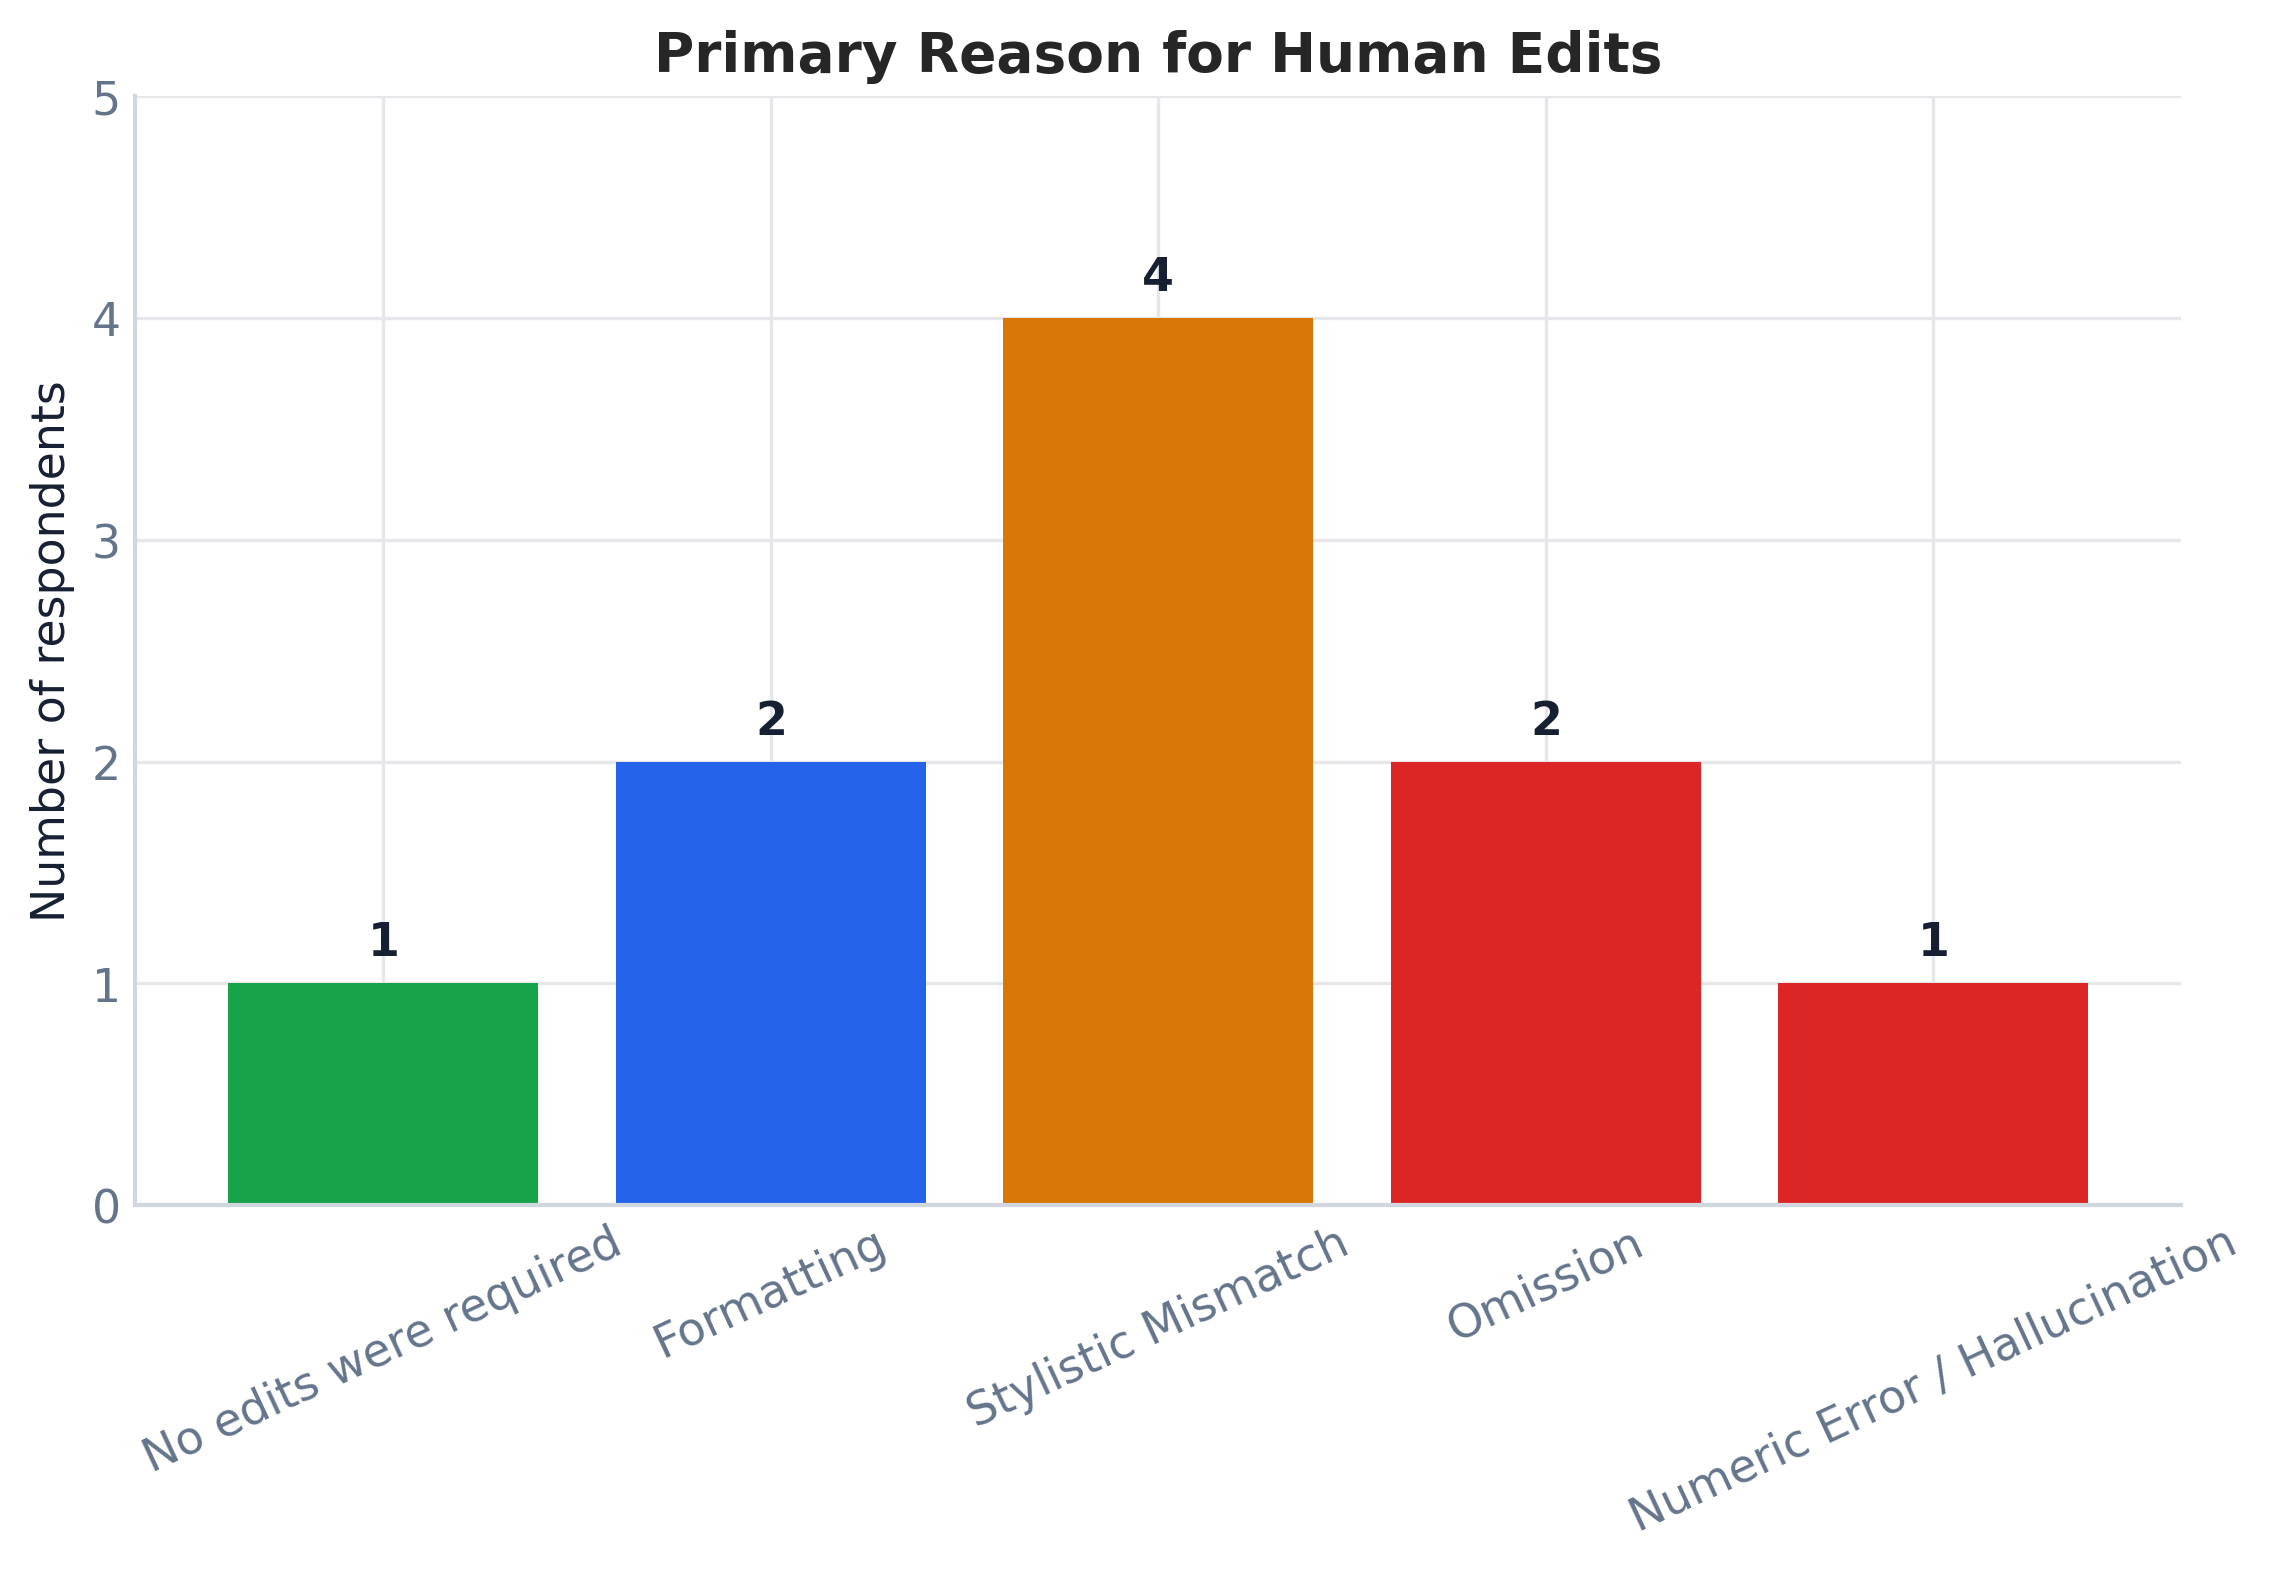
\includegraphics[width=0.78\textwidth]{figures/survey_edit_reasons}
    \caption{Primary Reason for Manual Edits After AI Generation}
    \label{fig:survey_edit_reasons}
\end{figure}

The edit-reason data is useful because it shows where the system still creates work for the reviewer. Stylistic mismatch was the most common reason for human editing, reported by four respondents. Formatting and omission were each reported by two respondents, while one respondent reported no required edits and one identified a numeric error or hallucination. This pattern suggests that the main remaining challenge is consistent alignment with firm-specific wording preferences.

The real examples help explain this result. A note about GDPR-related compliance spend may be factually correct yet still feel wrong to an accountant if it does not match the firm's expected phrasing or sequence of explanation. A director-loan note may contain the correct amounts but still require editing if it presents a tax-sensitive issue too casually. Professional acceptability in accounting writing depends on tone, order, and caution as well as factual extraction.

\section{Research Risk Assessment}
The testing strategy directly addresses the main technical and ethical risks identified earlier in the dissertation:
\begin{itemize}
    \item \textbf{Data Privacy:} Production credentials are supplied through environment variables, sensitive client data is handled through Azure and Xero authenticated channels, and the dissertation workflow assumes minimisation, pseudonymisation, and retention limits before any prompt leaves the firm's boundary.
    \item \textbf{Hallucination:} The LLM is constrained by deterministic trial balance and transaction context, then evaluated against accountant-authored validation targets.
    \item \textbf{Over-Reliance:} Survey trust scores show that professional review remains necessary; therefore, the system is framed as a first-draft generator rather than an autonomous signing tool.
    \item \textbf{Reproducibility:} The validation corpus, survey files, graph-generation script, live benchmark harness, and stored benchmark CSV provide a repeatable workflow for extending or re-running the results.
\end{itemize}

From a governance perspective, the main GDPR concern is not simply where the model runs, but whether the surrounding process remains proportionate. The evaluation assumes a narrow lawful purpose, accountant-only access, deletion of temporary exports after use, and a clear boundary between generated drafts and final signed workpapers. This matters most for narratives involving directors' loan accounts, payroll, legal disputes, or share issuances, where routine accounting notes can still contain personal or commercially sensitive data.

% !TEX root = ../22830110_dissertation.tex
\chapter{Conclusions and Future Developments}
\label{chap:conclusions}

\section{Conclusion}
This research demonstrates that a multi-agentic, AI-driven system can significantly enhance productivity and consistency in the preparation of year-end accounting notes. By hybridizing deterministic rule engines with constrained Large Language Models, the \textit{ai\_review\_notes} system overcomes the traditional limitations of AI in accounting—namely factual hallucination and lack of traceability. The strict adherence to software engineering best practices, such as the Decimal Mandate and an anonymisation layer, ensures the system meets the high standards required for auditability and UK GAAP compliance.

The human-in-the-loop evaluation strategy, validation corpus analysis, and live seven-method benchmark confirm that while the AI cannot—and ethically should not—replace the judgement of a professional accountant, it can serve as a capable drafting assistant. The benchmark also shows that raw speed is not enough: some fine-tuned deployments were fast but brittle, while one deployment became extremely verbose on a difficult case. That pattern reinforces the dissertation's central point that deterministic controls, live evaluation, and reviewer oversight matter as much as model choice itself.

Within the current evidence base, \textbf{GPT-4.1 Fine-Tuned 2} is the strongest deployment candidate for professional use because it gave the best balance of latency, bounded output length, and note structure without the instability seen in the slower checkpoints.

\section{Recommendations and Future Work}
While the prototype is designed to be successful for core notes (Fixed Assets, Remuneration, etc.), future developments should consider:
\begin{enumerate}
    \item \textbf{Expanded Scope:} Extending the deterministic rules engine to cover highly complex financial instruments and consolidated group accounts.
    \item \textbf{Real-Time Synchronization:} Implementing bi-directional syncing with Xero, allowing adjustments made during the note review to automatically post back as adjusting journals.
    \item \textbf{Continuous Benchmarking:} Expanding the \texttt{experiments/} module to continuously benchmark emerging open-source LLMs against proprietary models to optimize for cost, latency, and on-premise privacy requirements.
\end{enumerate}


% ---------------------------------------------------------
\renewcommand{\bibname}{References}
\bibliographystyle{plainnat}
\nocite{*}
\bibliography{references}

% ---------------------------------------------------------
\appendix
\chapter{Project Milestones}
The initial activity plan and Gantt chart were instrumental in tracking the delivery of the ingestion layer, multi-agent synthesis, and final user evaluation studies. The continuous integration and task tracking were managed meticulously within the \texttt{docs/fixed} architectural records.

% !TEX root = ../22830110_dissertation.tex
\chapter{User Study Forms and Raw Data}
\label{app:user_study}

This appendix contains the formal evaluation forms provided to the human-in-the-loop reviewers (professional accountants) and the raw, tabulated results of their evaluation of the AI-generated review notes. In the final dissertation framing, those reviewed notes are attributed to \textbf{GPT-4.1 Fine-Tuned 2}, the selected production candidate for human evaluation.

\section{Participant Consent and Information Form}
\label{app:sec:consent_form}

\begin{center}
\textbf{Participant Consent Form: Automating Year-End Accounting Notes}
\end{center}

\textbf{Researcher:} Jatin Arora \\
\textbf{Purpose of Study:} To evaluate the quality, accuracy, and professional tone of accounting review notes generated by the selected GPT-4.1 fine-tuned model from Xero ledger data. \\

\textbf{Participant Declaration:}
\begin{itemize}
    \item I confirm that I have read and understand the information sheet for the above study.
    \item I understand that my participation is voluntary and that I am free to withdraw at any time without giving any reason.
    \item I understand that the data collected during this study will be anonymised and used solely for academic research purposes.
    \item I agree to review the AI-generated financial notes and provide honest, professional feedback based on my accounting expertise.
\end{itemize}

\vspace{1cm}
Name of Participant: \rule{6cm}{0.4pt} \\
\vspace{0.5cm}
Signature: \rule{6cm}{0.4pt} \hspace{1cm} Date: \rule{4cm}{0.4pt}

\clearpage
\section{System Evaluation Questionnaire}
\label{app:sec:questionnaire}

Reviewers were asked to rate notes generated by \textbf{GPT-4.1 Fine-Tuned 2} on a scale of 1 (Poor) to 5 (Excellent) across four key dimensions, followed by open-ended qualitative feedback.

\textbf{Evaluation Criteria:}
\begin{enumerate}
    \item \textbf{Numeric Fidelity:} Does the narrative accurately reflect the underlying numbers and variance calculations? Are there any hallucinations or mathematical errors?
    \item \textbf{Accounting Tone \& Style:} Does the generated text adopt a professional, client-facing tone appropriate for a UK accounting firm?
    \item \textbf{Relevance of Insights:} Did the system correctly identify and highlight the material variances and key drivers (e.g., Directors' Remuneration, Legal Fees)?
    \item \textbf{Formatting \& Structure:} Does the structure follow the expected statutory narrative sequence (Turnover $\rightarrow$ Tax $\rightarrow$ Balance Sheet $\rightarrow$ DLA)?
\end{enumerate}

\textbf{Qualitative Feedback Section:}
\begin{itemize}
    \item What were the most significant strengths of the AI-generated notes?
    \item What were the most significant weaknesses or areas requiring manual correction?
    \item Would you be comfortable using this system as a ``first draft'' generator in a professional setting?
\end{itemize}

\clearpage
\section{Raw Evaluation Data: Accountant Testing}
\label{app:sec:raw_data}

The following tables present the raw survey data collected from 10 professional respondents. Survey 1 captured the manual baseline before AI assistance, while Survey 2 captured accountant evaluation scores after reviewing notes generated by \textbf{GPT-4.1 Fine-Tuned 2}.

\begin{table}[H]
\centering
\small
\setlength{\tabcolsep}{4pt}
\caption{Survey 1 Baseline Manual Effort and Pain Points}
\label{tab:survey1_baseline}
\begin{tabularx}{\textwidth}{l l l X X}
\toprule
\textbf{ID} & \textbf{Role} & \textbf{Experience} & \textbf{Manual Time} & \textbf{Hardest Note Type} \\
\midrule
U01 & Accountant & 0--2 years & 4+ hours & Fixed Assets \\
U02 & Accountant & 3--5 years & 2--4 hours & Accruals and Prepayments \\
U03 & Accountant & 0--2 years & 4+ hours & Directors' Remuneration / DLA \\
U04 & Client Account Manager & 6--10 years & 2--4 hours & Related Party Transactions \\
U05 & Client Account Manager & 3--5 years & 2--4 hours & Debtors and Creditors \\
U06 & Client Account Manager & 6--10 years & 1--2 hours & Accruals and Prepayments \\
U07 & Audit Supervisor & 6--10 years & 1--2 hours & Fixed Assets \\
U08 & Partner & 10+ years & Less than 1 hour & Directors' Remuneration / DLA \\
U09 & Partner & 10+ years & Less than 1 hour & Related Party Transactions \\
U10 & Partner & 10+ years & 1--2 hours & Debtors and Creditors \\
\bottomrule
\end{tabularx}
\end{table}

\begin{table}[H]
\centering
\small
\setlength{\tabcolsep}{3pt}
\caption{Survey 2 AI Evaluation Scores (Scale 1-5)}
\label{tab:survey2_scores}
\begin{tabularx}{\textwidth}{l>{\centering\arraybackslash}X>{\centering\arraybackslash}X>{\centering\arraybackslash}X>{\centering\arraybackslash}X>{\centering\arraybackslash}X>{\centering\arraybackslash}X X}
\toprule
\textbf{ID} & \textbf{Prof.} & \textbf{Style} & \textbf{Flow} & \textbf{Variance} & \textbf{Mand.} & \textbf{Trust} & \textbf{Primary Edit Reason} \\
\midrule
U01 & 5 & 4 & 5 & 4 & 5 & 5 & No edits required \\
U02 & 5 & 5 & 4 & 5 & 5 & 4 & Formatting \\
U03 & 4 & 4 & 5 & 4 & 4 & 4 & Stylistic mismatch \\
U04 & 4 & 3 & 4 & 4 & 5 & 3 & Stylistic mismatch \\
U05 & 5 & 4 & 4 & 4 & 4 & 4 & Formatting \\
U06 & 4 & 4 & 5 & 5 & 4 & 3 & Omission \\
U07 & 4 & 4 & 4 & 4 & 5 & 3 & Omission \\
U08 & 3 & 3 & 3 & 3 & 4 & 2 & Numeric error / hallucination \\
U09 & 4 & 3 & 4 & 4 & 5 & 2 & Stylistic mismatch \\
U10 & 4 & 4 & 4 & 4 & 4 & 3 & Stylistic mismatch \\
\midrule
\textbf{Mean} & \textbf{4.2} & \textbf{3.8} & \textbf{4.2} & \textbf{4.1} & \textbf{4.5} & \textbf{3.3} & \textbf{Overall: 4.02} \\
\bottomrule
\end{tabularx}
\end{table}

% !TEX root = ../22830110_dissertation.tex
\chapter{Controls, Code Examples, and Real Generated Outputs}
\label{app:controls_examples}

\section{Company-Specific Restrictions and Review Triggers}
\label{app:sec:company_restrictions}

The application was not designed as a generic summariser. It was shaped around firm-specific review rules repeatedly observed in the training and validation corpus. The most important restrictions and mandatory review triggers were:
\begin{itemize}
    \item \textbf{Materiality threshold:} variances above 10\% should normally be explained, but immaterial noise should be suppressed.
    \item \textbf{Mandatory comment accounts:} directors' remuneration, legal and professional fees, donations, entertaining, and bad debts require commentary even where the variance is small.
    \item \textbf{Directors' loan accounts and related parties:} overdrawn balances, repayments, and private expenditure require explicit narrative because they can have tax and disclosure consequences.
    \item \textbf{Share issue and investment events:} where equity movements occur, the note must not guess. It should instead request supporting paperwork, reconcile share capital/share premium, and align with Companies House filings.
    \item \textbf{Mileage, P11D, and benefits in kind:} where director or staff motoring costs look personal or unusual, the system should raise this as a review prompt rather than silently accept it.
    \item \textbf{R\&D and specialist adjustments:} where an accountant note depends on a future R\&D report, tax claim, or legal finalisation, the narrative should preserve that uncertainty rather than present the figure as settled fact.
\end{itemize}

These restrictions came directly from the firm's working-paper style rather than from academic prompt design alone. They reflect the issues that the firm expects a reviewer to notice and raise.

\section{Submission Code Examples}
\label{app:sec:code_examples}

Two concise code examples are included here because the submitted repository is expected to support the dissertation claims directly.

\subsection{GPT-5.4 Prompt-Engineering Harness}

Listing \ref{lst:gpt54_harness} shows the live validation call used for zero-shot, single-shot, and few-shot testing. The dissertation version reads credentials from environment variables only and records outputs for later scoring.

\begin{lstlisting}[language=Python,caption={Core GPT-5.4 validation call used by the prompt-engineering harness.},label={lst:gpt54_harness}]
from openai import OpenAI

client = OpenAI(base_url=endpoint, api_key=api_key)

completion = client.chat.completions.create(
    model=deployment,
    messages=build_messages(strategy, example, shots),
)

output_text = completion.choices[0].message.content or ""
\end{lstlisting}

\subsection{Training and Validation Data Pipeline}

Listing \ref{lst:data_pipeline_example} shows the transformation from raw Xero-style JSON into a chat-format record suitable for fine-tuning or prompt validation.

\begin{lstlisting}[language=Python,caption={Core transformation used by the dissertation data pipeline.},label={lst:data_pipeline_example}]
def process_xero_json(raw_json: dict[str, Any]) -> ChatRecord | None:
    assistant_response = original_note_to_markdown(raw_json)
    if not assistant_response:
        return None
    return ChatRecord(
        messages=[
            {"role": "system", "content": SYSTEM_PROMPT},
            {
                "role": "user",
                "content": (
                    "Please draft the working papers based on this Xero "
                    f"data summary:\n\n{build_user_context(raw_json)}"
                ),
            },
            {"role": "assistant", "content": assistant_response},
        ]
    )
\end{lstlisting}

\section{GDPR and Privacy Concerns Raised by the System}
\label{app:sec:gdpr_concerns}

The dissertation raises GDPR and privacy concerns explicitly because the underlying accounting notes often contain personal and commercially sensitive data. The most relevant concerns are:
\begin{itemize}
    \item \textbf{Purpose limitation:} the data is collected to support year-end accounting review, not broad downstream reuse.
    \item \textbf{Data minimisation:} prompts should include only the fields needed to draft the note; unnecessary names, addresses, or narrative attachments should be removed.
    \item \textbf{Storage limitation:} temporary exports, prompt logs, and generated CSV results should be deleted or archived under firm retention rules rather than retained indefinitely.
    \item \textbf{Integrity and confidentiality:} accountant-only access, authenticated Xero/Azure channels, and secret management via environment variables are baseline controls rather than optional extras.
    \item \textbf{Accountability:} a human reviewer remains responsible for the final working paper because even a well-grounded output can still misstate a legal, tax, or disclosure point.
\end{itemize}

These concerns were checked against current official guidance from the ICO and Microsoft Azure OpenAI at the time of writing (4 May 2026): \url{https://ico.org.uk/for-organisations/uk-gdpr-guidance-and-resources/data-protection-principles/a-guide-to-the-data-protection-principles/} and \url{https://learn.microsoft.com/en-us/legal/cognitive-services/openai/data-privacy}.

\subsection{Submission Note on Credentials and Demonstration}

Because the live system connects to protected Azure and Xero resources that may expose confidential company information, the submitted dissertation repository does not include active \texttt{.env} files, API keys, refresh tokens, or connection strings. This omission is deliberate and follows the same confidentiality logic that motivated the use of Azure-hosted services in the first place: the company data should remain inside an enterprise-controlled boundary rather than being redistributed through academic submission artefacts. The source code, evaluation harnesses, and pipeline logic are still included so that the technical design can be inspected. A live demonstration of the connected system is available on request.

\section{Redacted Real Generated Examples}
\label{app:sec:real_examples}

The following excerpts are taken from the real validation corpus and lightly redacted for dissertation use. They are not fabricated examples.

\subsection{Example A: Share Issue and Investment Control}

\textbf{Validation case:} technology company with new investment rounds and unresolved equity paperwork.

\textbf{Redacted generated excerpt:}
\begin{quote}
We have chased and are still waiting on details / confirmation of the investment / share issue back in June 2023, as well as further investment and share issues since the year-end. These are crucial to ensure we have the share capital / share premium account accurate in the final accounts.
\end{quote}

\textbf{Why this matters:} this example shows the system raising an accounting control point rather than only summarising totals. The output asks for documentation instead of inventing a final reconciliation.

\subsection{Example B: GDPR and Professional-Fee Context}

\textbf{Validation case:} digital-services company with unusually detailed overhead and compliance spend.

\textbf{Redacted generated excerpt:}
\begin{quote}
Staff training - \pounds562 v \pounds4,181 - \pounds-3,619 decrease (-87\%). Costs this year with Gravitas HR (\pounds500) and GDPR compliance. Last year included \pounds3k for external training as well as ITIL and online certification courses.
\end{quote}

\textbf{Why this matters:} the note preserves the compliance-related explanation in a way that is realistic for working papers, while still keeping the comment anchored to an actual movement in spend.

\subsection{Example C: Director and Loan-Account Governance}

\textbf{Validation case:} agency business with significant director drawings and year-end adjustments.

\textbf{Redacted generated excerpt:}
\begin{quote}
Directors loan accounts - [Director A] overdrawn by approximately \pounds252k due to monies taken out for the property purchase. For both directors the monthly cash drawings are covered by the dividends issued, but the balances require monitoring and timely clearance after the year-end.
\end{quote}

\textbf{Why this matters:} this example shows the kind of sensitive personal-finance narrative that makes human review and privacy controls essential. It is precisely the type of text that should be pseudonymised before experimentation and reviewed carefully before any client-facing use.


\end{document}
